\section{Application of Allele-specific models to the METABRIC data}
In this Chapter, allele-specific copy number profiles for 1,984 patients in the METABRIC cohort are produced, the frequency of changepoints across defined intervals examined, and the selected statistical models, ADIM fitted using the \texttt{lm()} and \texttt{MCMCglmm()} functions, applied to identify regions containing CNA changepoints of significant length. Here, the observed interval $d$ is either a gene region, i.e. between the start and end position of a gene, referred to as gene-centric, or genomic segments of specified length generated using a segmentation approach.  

\subsection{Gene-centric Application of Allele-specific Profile Analysis}
Gene-centric changepoints (changepoints that occur in genes) in allele-specific CNA profiles are examined using visualisations and application of AD models.

\subsubsection{Gene-centric Allele-specific CNA State Heatmaps}
The CNA landscape of allele-specific copy number profiles, in terms of the CNA state of each gene, on each allele, are visualised using heatmaps.

In Section \ref{Heatmaps_Chap3}, heatmaps were implemented based on aggregate total CNA data, of particular interest was chromosome 3p, where the patients were partitioned into nodes informed by chromosome arm CNA Burden metrics (Figure \ref{PA_SurvTrees_Burden_Heatmaps_3p}). Allele-specific profiles are now provided, that is, for the 3p Major allele (Figure \ref{fig:heatmap_Major}) and for the 3p Minor allele (Figure \ref{fig:heatmap_Minor}). The CNA states correspond to -1 (deletion), 0 (neutral), 1 (gain) and 2 (amplification).

Figure \ref{fig:heatmap_Major} indicates subsets of patients displaying amplifications in almost every gene on the Major allele across chromosome 3p, while Figure \ref{fig:heatmap_Minor} indicates clusters of patients displaying either amplifications or deletions in almost every gene on the Minor allele across chromosome 3p. These heatmaps indicate that amplifications are more prevalent on the Major allele, while deletions tend to occur more on the Minor allele. This is not surprising given that the Minor allele is defined as the allele with the lowest copy number across the genome. Notably, the deletions observed across chromosome 3p utilising total CNA states occur on a single allele, the Minor allele (Figure \ref{PA_SurvTrees_Burden_Heatmaps_3p}). 

Combining the allele-specific CNA states, by adding the individual allele states for the gene, shown in Figure \ref{fig:heatmap_Both}, shows some similarities to that generated using total copy number data (Figure \ref{PA_SurvTrees_Burden_Heatmaps_3p}). In both heatmaps, the Claudin-low and Luminal A patients corresponding to Node 5 have high levels of deletions across chromosome 3p. The majority of Node 4, also containing Claudin-low and Luminal A patients, display little to no copy number changes across chromosome 3p and Node 2, containing Luminal B, HER2, Normal and Basal patients, consists of patients displaying variation in levels of GI across chromosome 3p. There are some noteworthy differences, however. The allele-specific data contains more patients displaying high levels of amplifications, possibly indicative of genome duplication, across chromosome 3p, particularly evident for Node 2 patients (Figures \ref{PA_SurvTrees_Burden_Heatmaps_3p} and \ref{fig:heatmap_Both}). These allele specific heatmaps also highlight the existence of copy number neutral changes. 

\vfill
\begin{figure}[H]
\vspace{0.5cm}
\centering
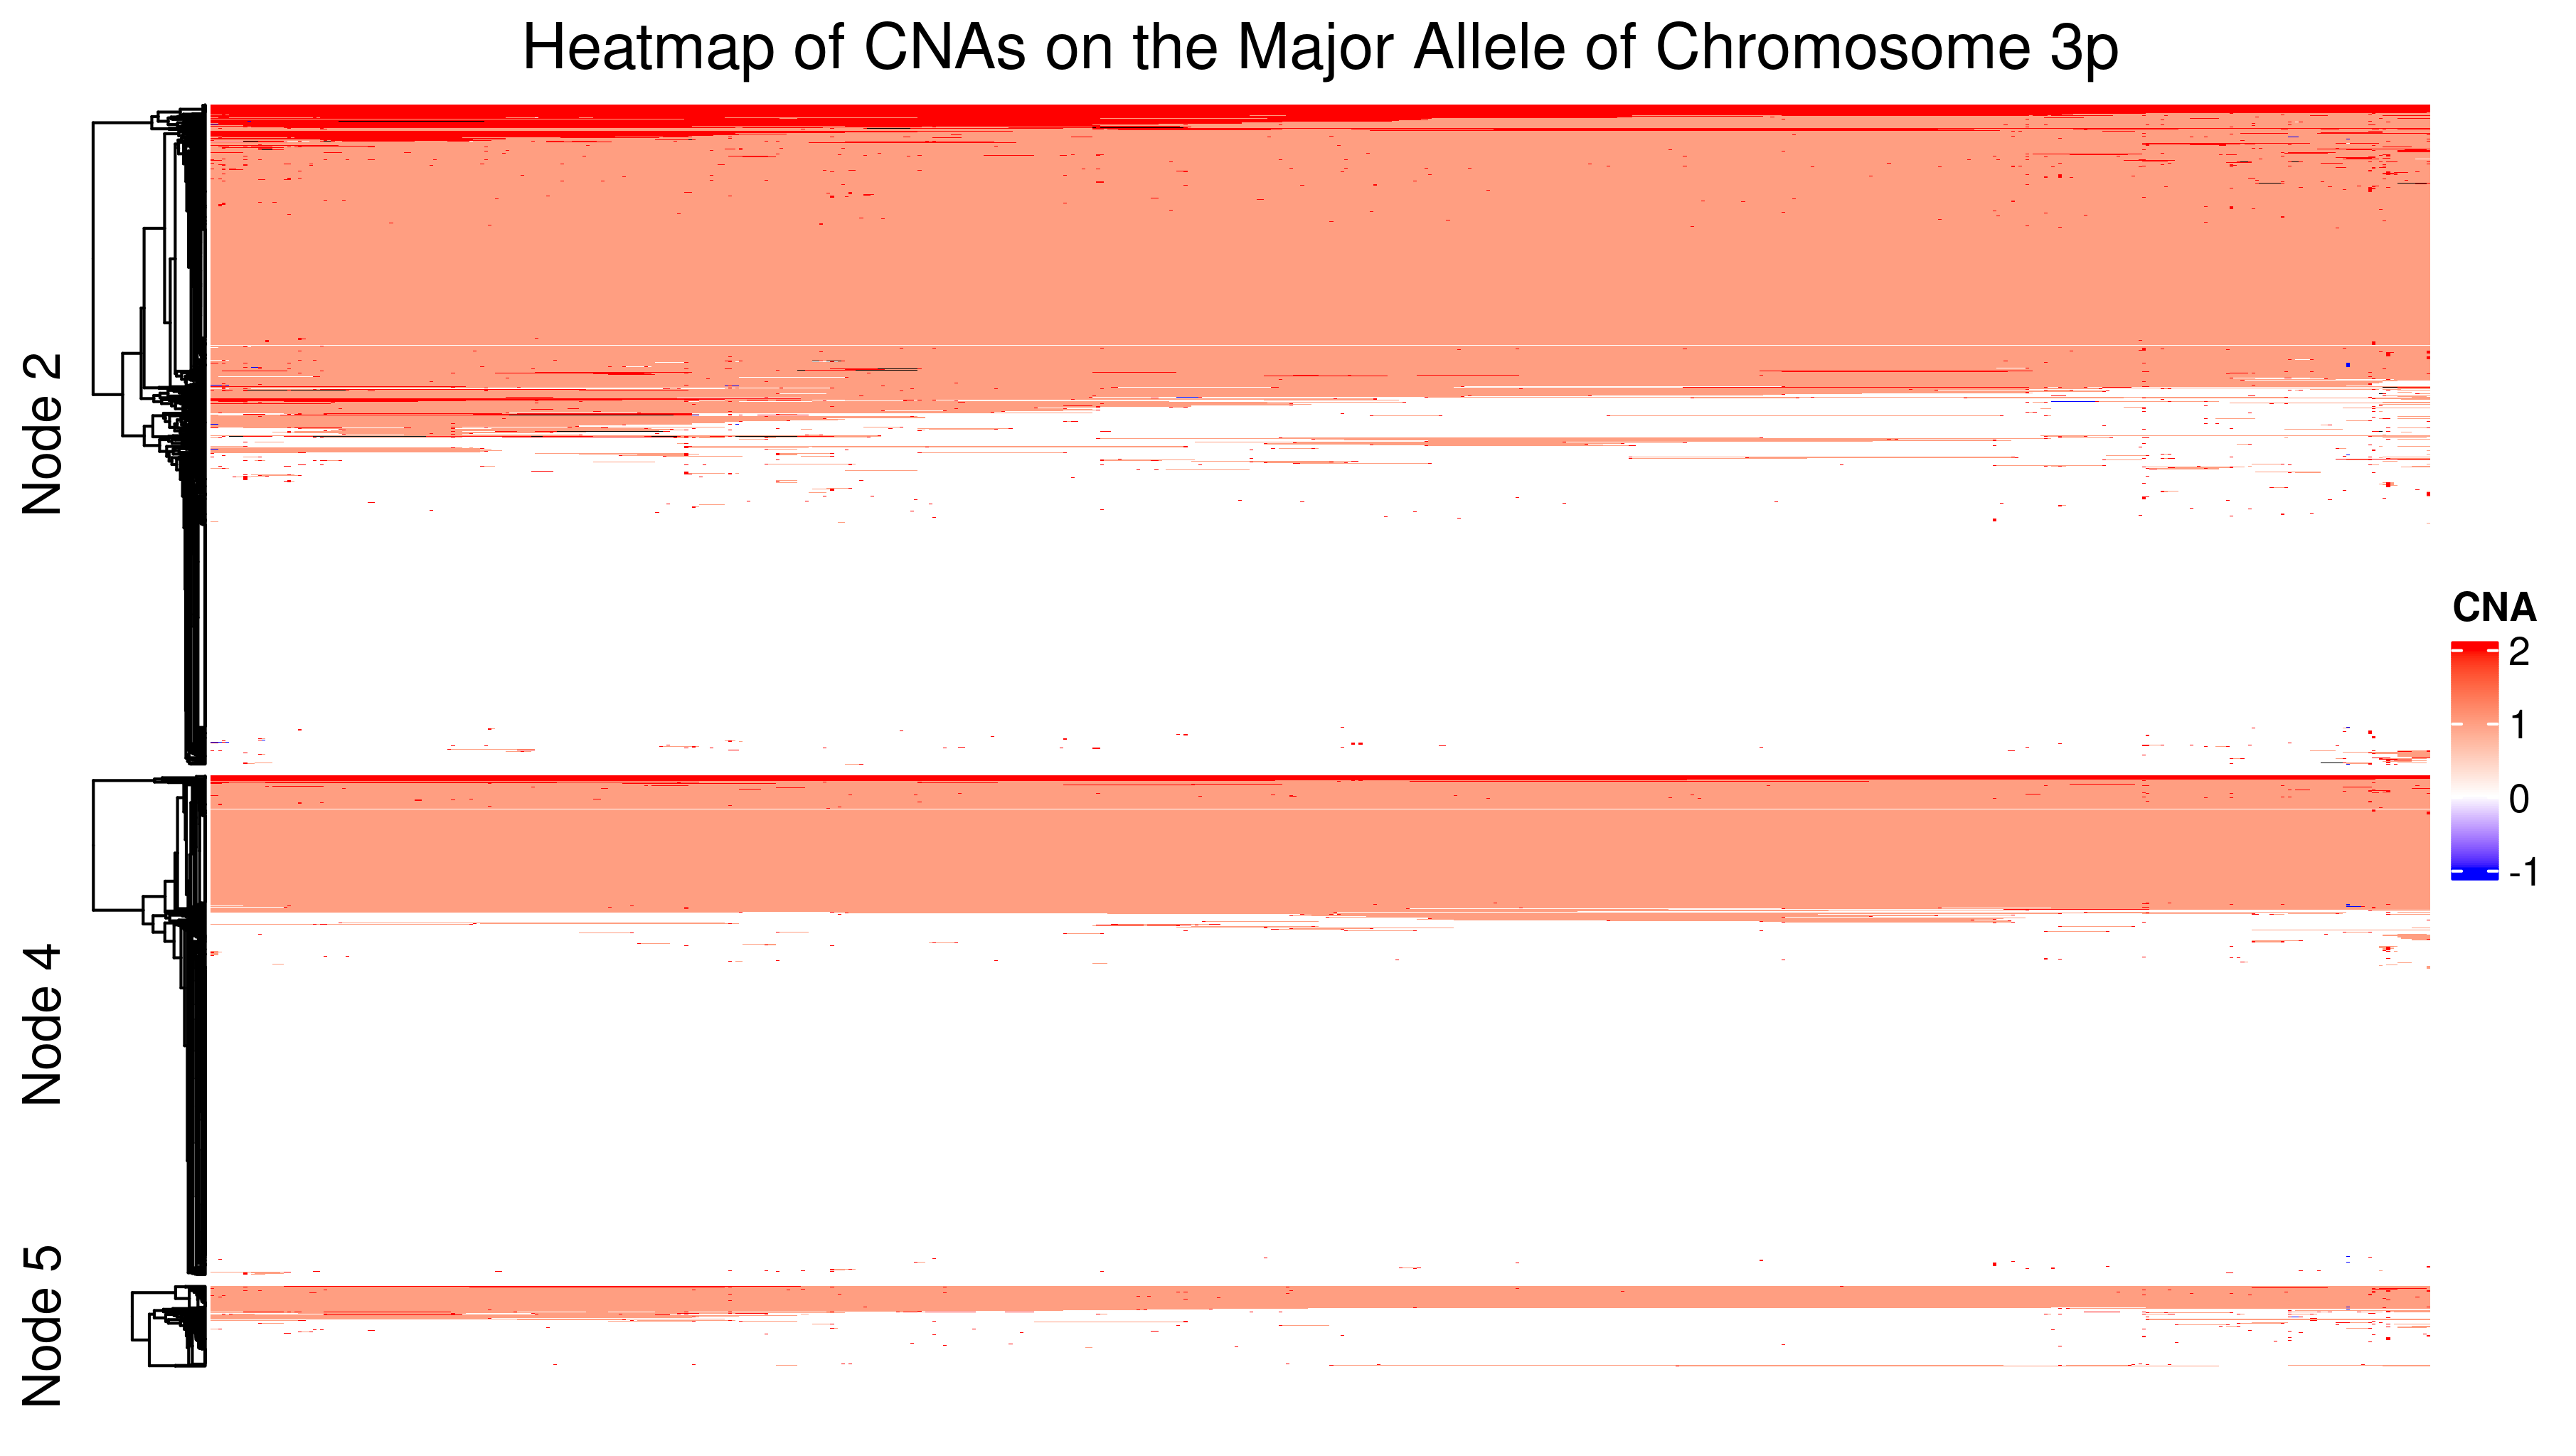
\includegraphics[width = 1\textwidth]{../figures/Chapter_6/Heatmap_Chr3p_Genes_Major.png}
\caption[Heatmap of CNAs across the Major Allele of Chromosome 3p]{Heatmap of CNAs across the Major Allele of Chromosome 3p. The heatmap depicts the CNA state for each gene across Chromosome 3p, partitioning the patients into the nodes corresponding to Figure \ref{fig:PAM50_PA_CNA_Burden_DSS}. NAs, depicting multiple states, are coloured in black.}
\label{fig:heatmap_Major}
\end{figure}
\vspace{0.5cm}
\begin{figure}[H]
\centering
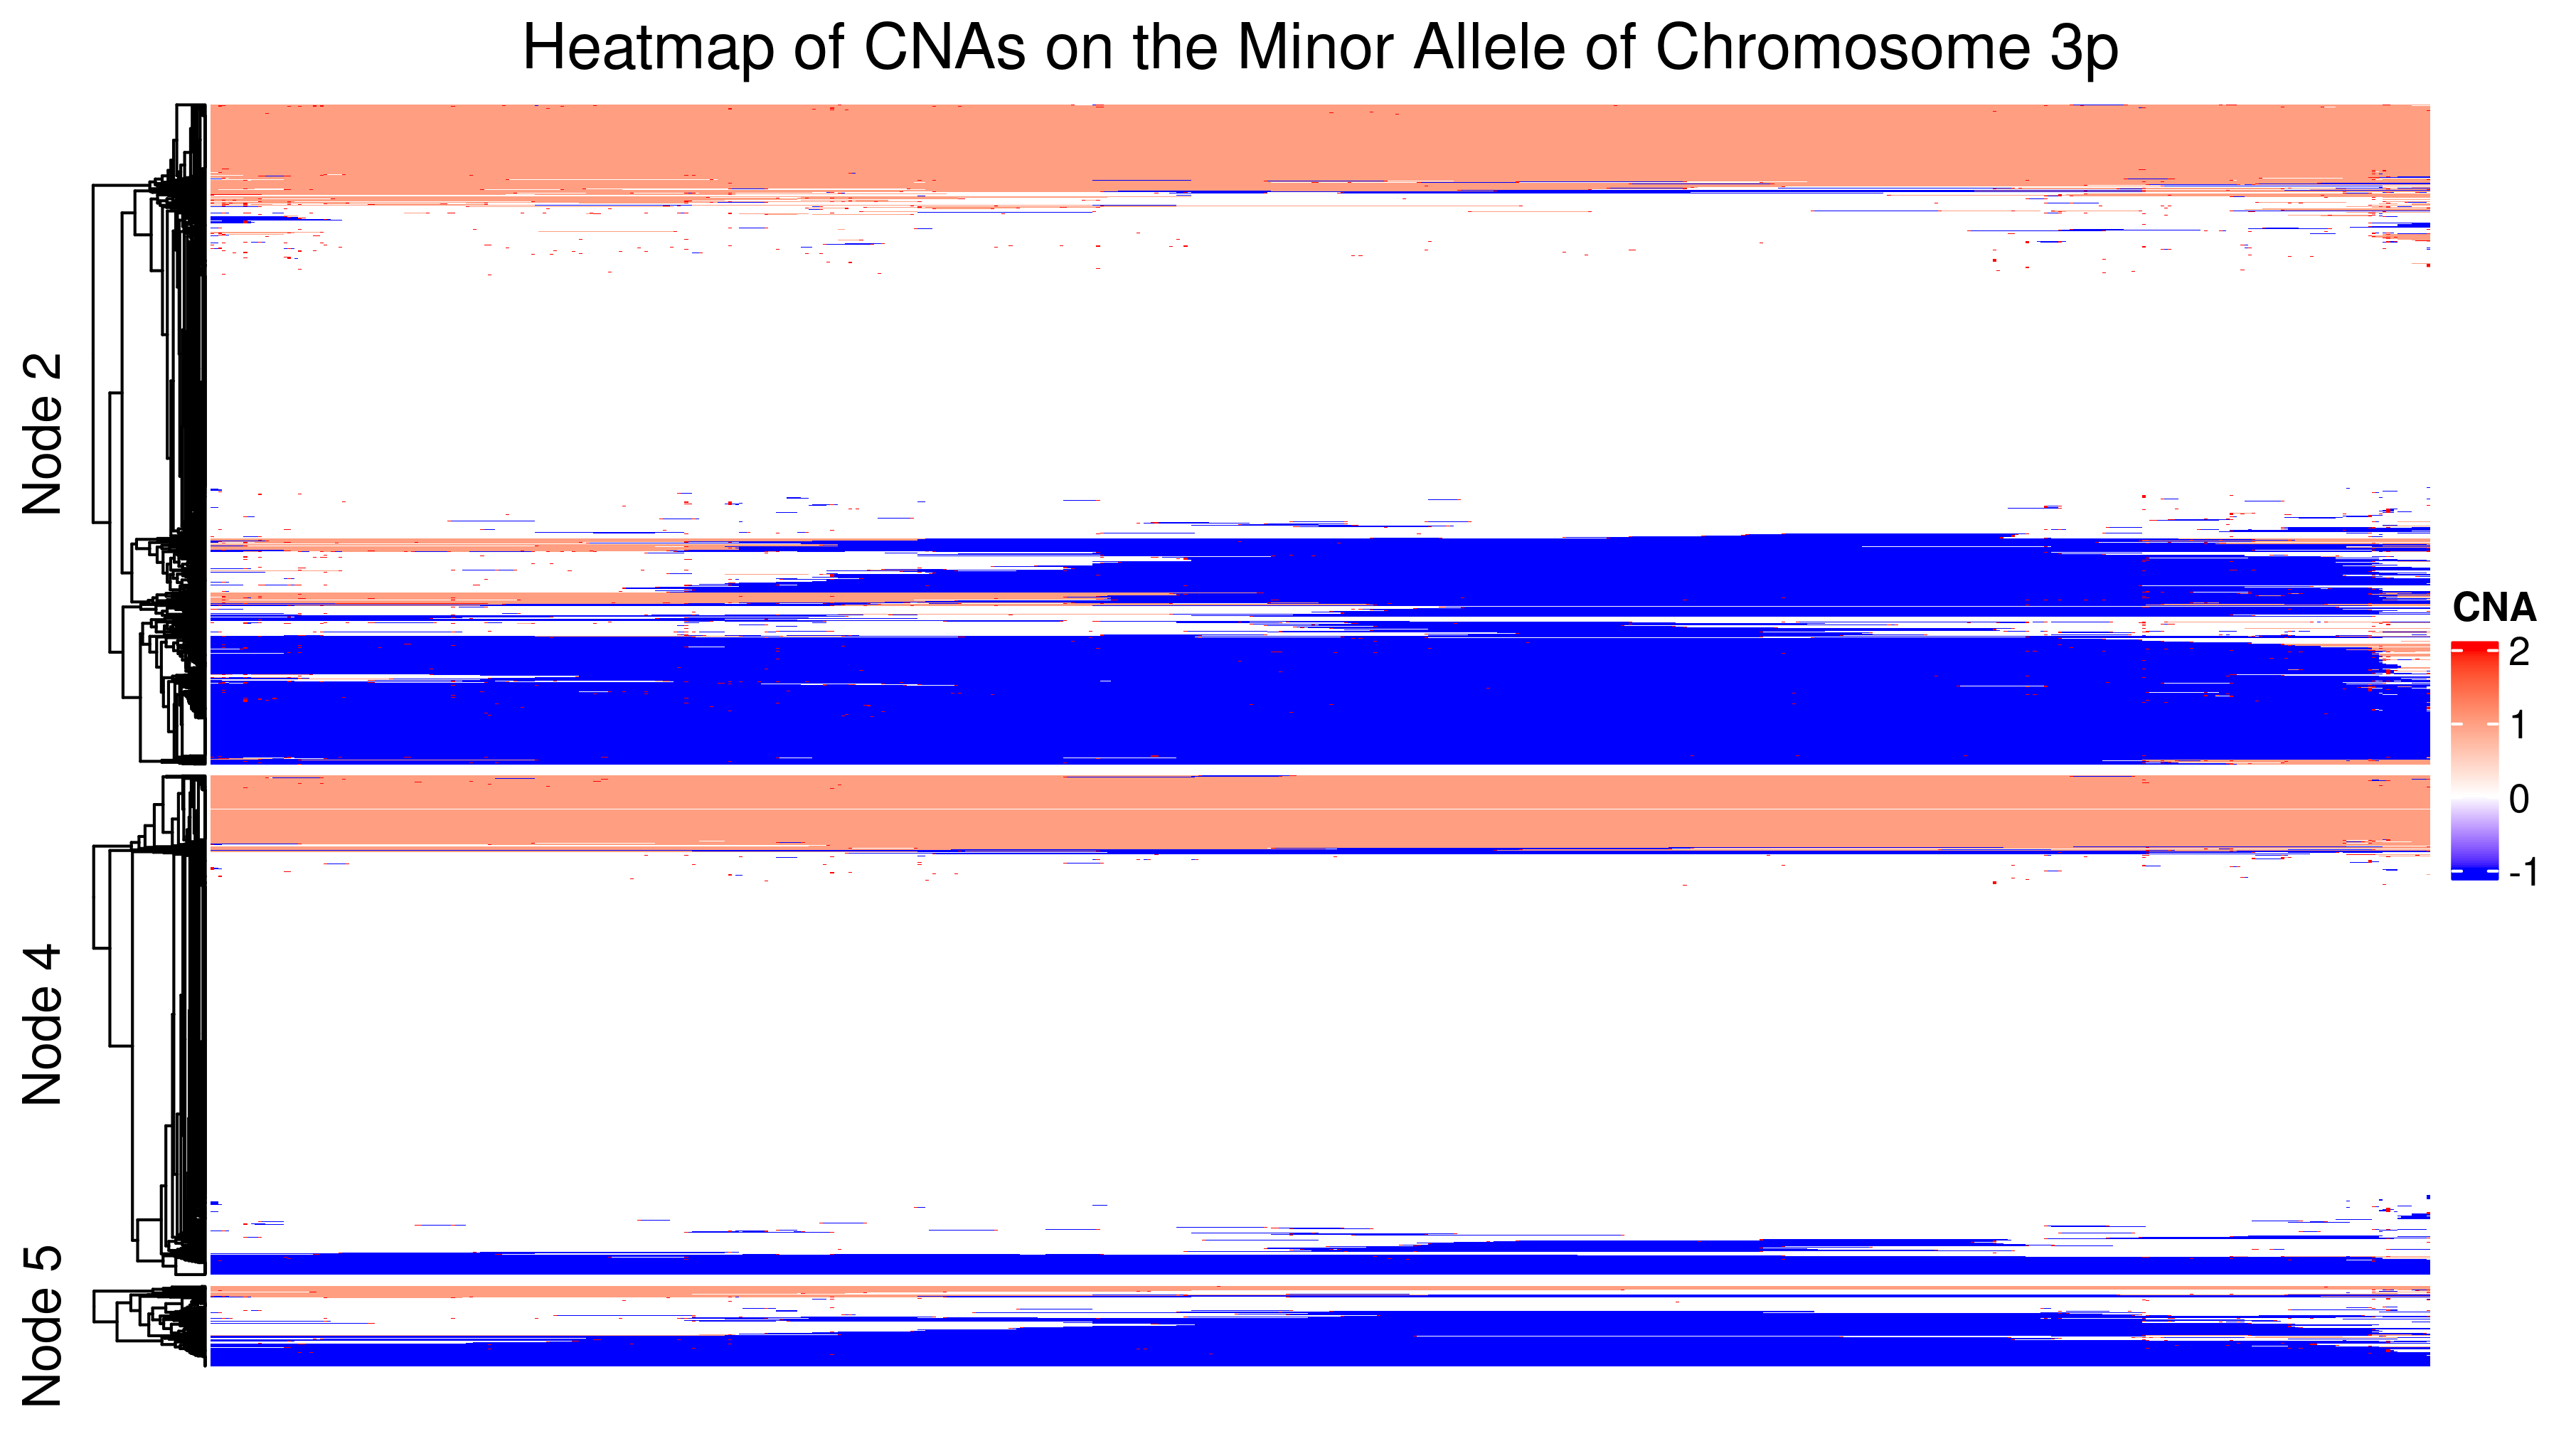
\includegraphics[width = 1\textwidth]{../figures/Chapter_6/Heatmap_Chr3p_Genes_Minor.png}
\caption[Heatmap of CNAs across the Minor Allele of Chromosome 3p]{Heatmap of CNAs across the Minor Allele of Chromosome 3p. The heatmap depicts the CNA state for each gene across Chromosome 3p, partitioning the patients into the nodes corresponding to Figure \ref{fig:PAM50_PA_CNA_Burden_DSS}. NAs, depicting multiple states, are coloured in black.}
\label{fig:heatmap_Minor}
\end{figure}
\vfill 

\begin{figure}[H]
\centering
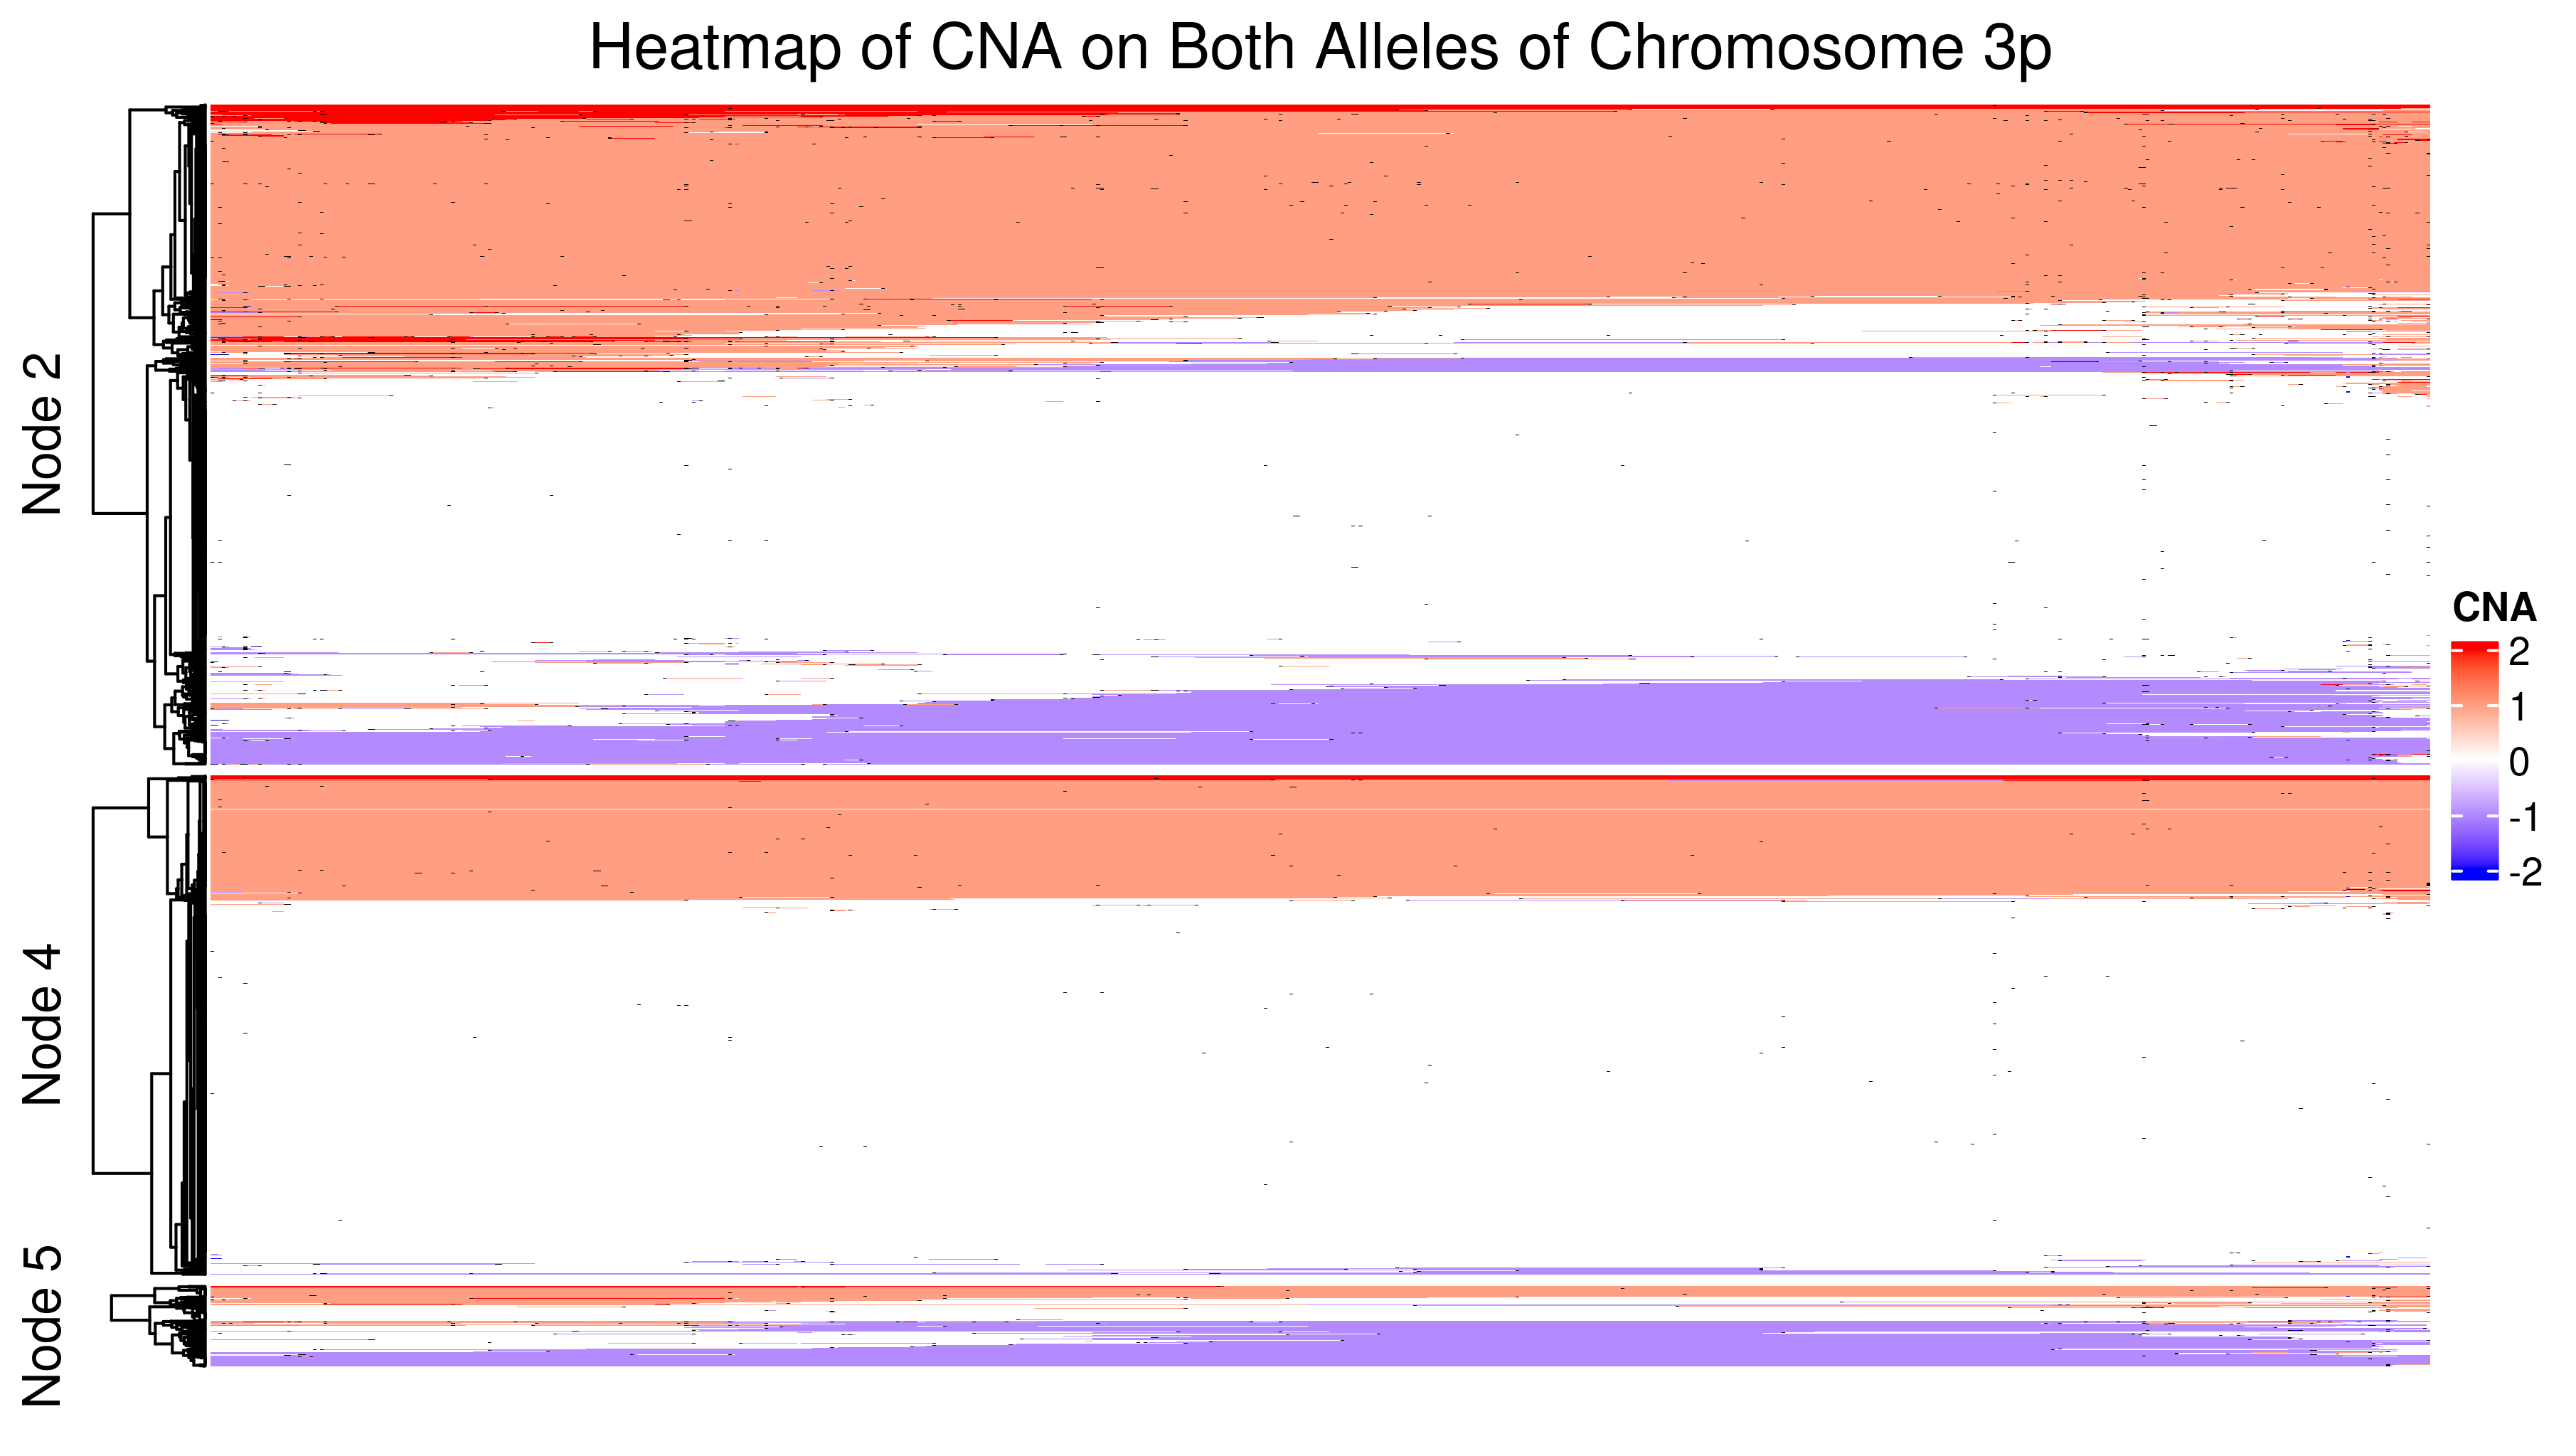
\includegraphics[width = 1\textwidth]{../figures/Chapter_6/Heatmap_Chr3p_Genes_Both_Alleles.png}
\caption[Heatmap of CNAs on both the Major and Minor alleles of Chromosome 3p]{Heatmap of CNAs on both the Major and Minor alleles of Chromosome 3p. The heatmap depicts the CNA state for each gene across Chromosome 3p, partitioning the patients into the nodes corresponding to Figure \ref{fig:PAM50_PA_CNA_Burden_DSS}. NAs, depicting multiple states, are coloured in black.}
\label{fig:heatmap_Both}
\end{figure}

Chromosome arms 18q and 11p were also a point of focus in analysing total CNAs in Section \ref{Heatmaps_Chap3} (Figure \ref{PA_SurvTrees_Burden_Heatmaps_18q}-\ref{PA_SurvTrees_Burden_Heatmaps_11p}). Allele-specific heatmaps produced for chromosome 18q and 11p, also indicate that the Major allele is dominated by amplification events, while the Minor allele, although displaying both amplifications and deletions, is primarily dominated by deletion events (Appendix F). Comparatively, ASCAT estimates fewer patients with widespread deletions across chromosomes and estimates more patients with widespread amplifications across chromosomes.

\subsubsection{Gene-centric Allelle-specific Changepoints across Chromosome Arms}
Figures \ref{fig:heatmap_Major}-\ref{fig:heatmap_Both} indicate that amplifications and deletions may occur because the whole length of the gene is amplified or deleted, denoted in red and blue, or because alterations (amplifications and/or deletions) occur at some point(s) within the gene, denoted in black. 

The frequency of changepoint events in genes on chromosome 3p, determined by the summation of observed changepoint counts over all patients, within each gene, is provided in Figure \ref{fig:Barplot_3p} where panels provide survival tree node and changepoint category information. These changepoint events, with the potential to disrupt gene function, tend to be observed with similar frequencies across all categories within each node, except for the Amp/Del and Del/Amp categories, which occur less frequently. Again, it is observed that Neut/Del and Del/Neut events occur more often on the Minor allele and Amp/Neut and Neut/Amp events occur more often on the Major allele. 

For Node 2, comprising 1,044 patients, the frequency of observed changepoints is quite low, with the gene displaying the highest total number of changepoints being 

\begin{figure}[H]
\centering

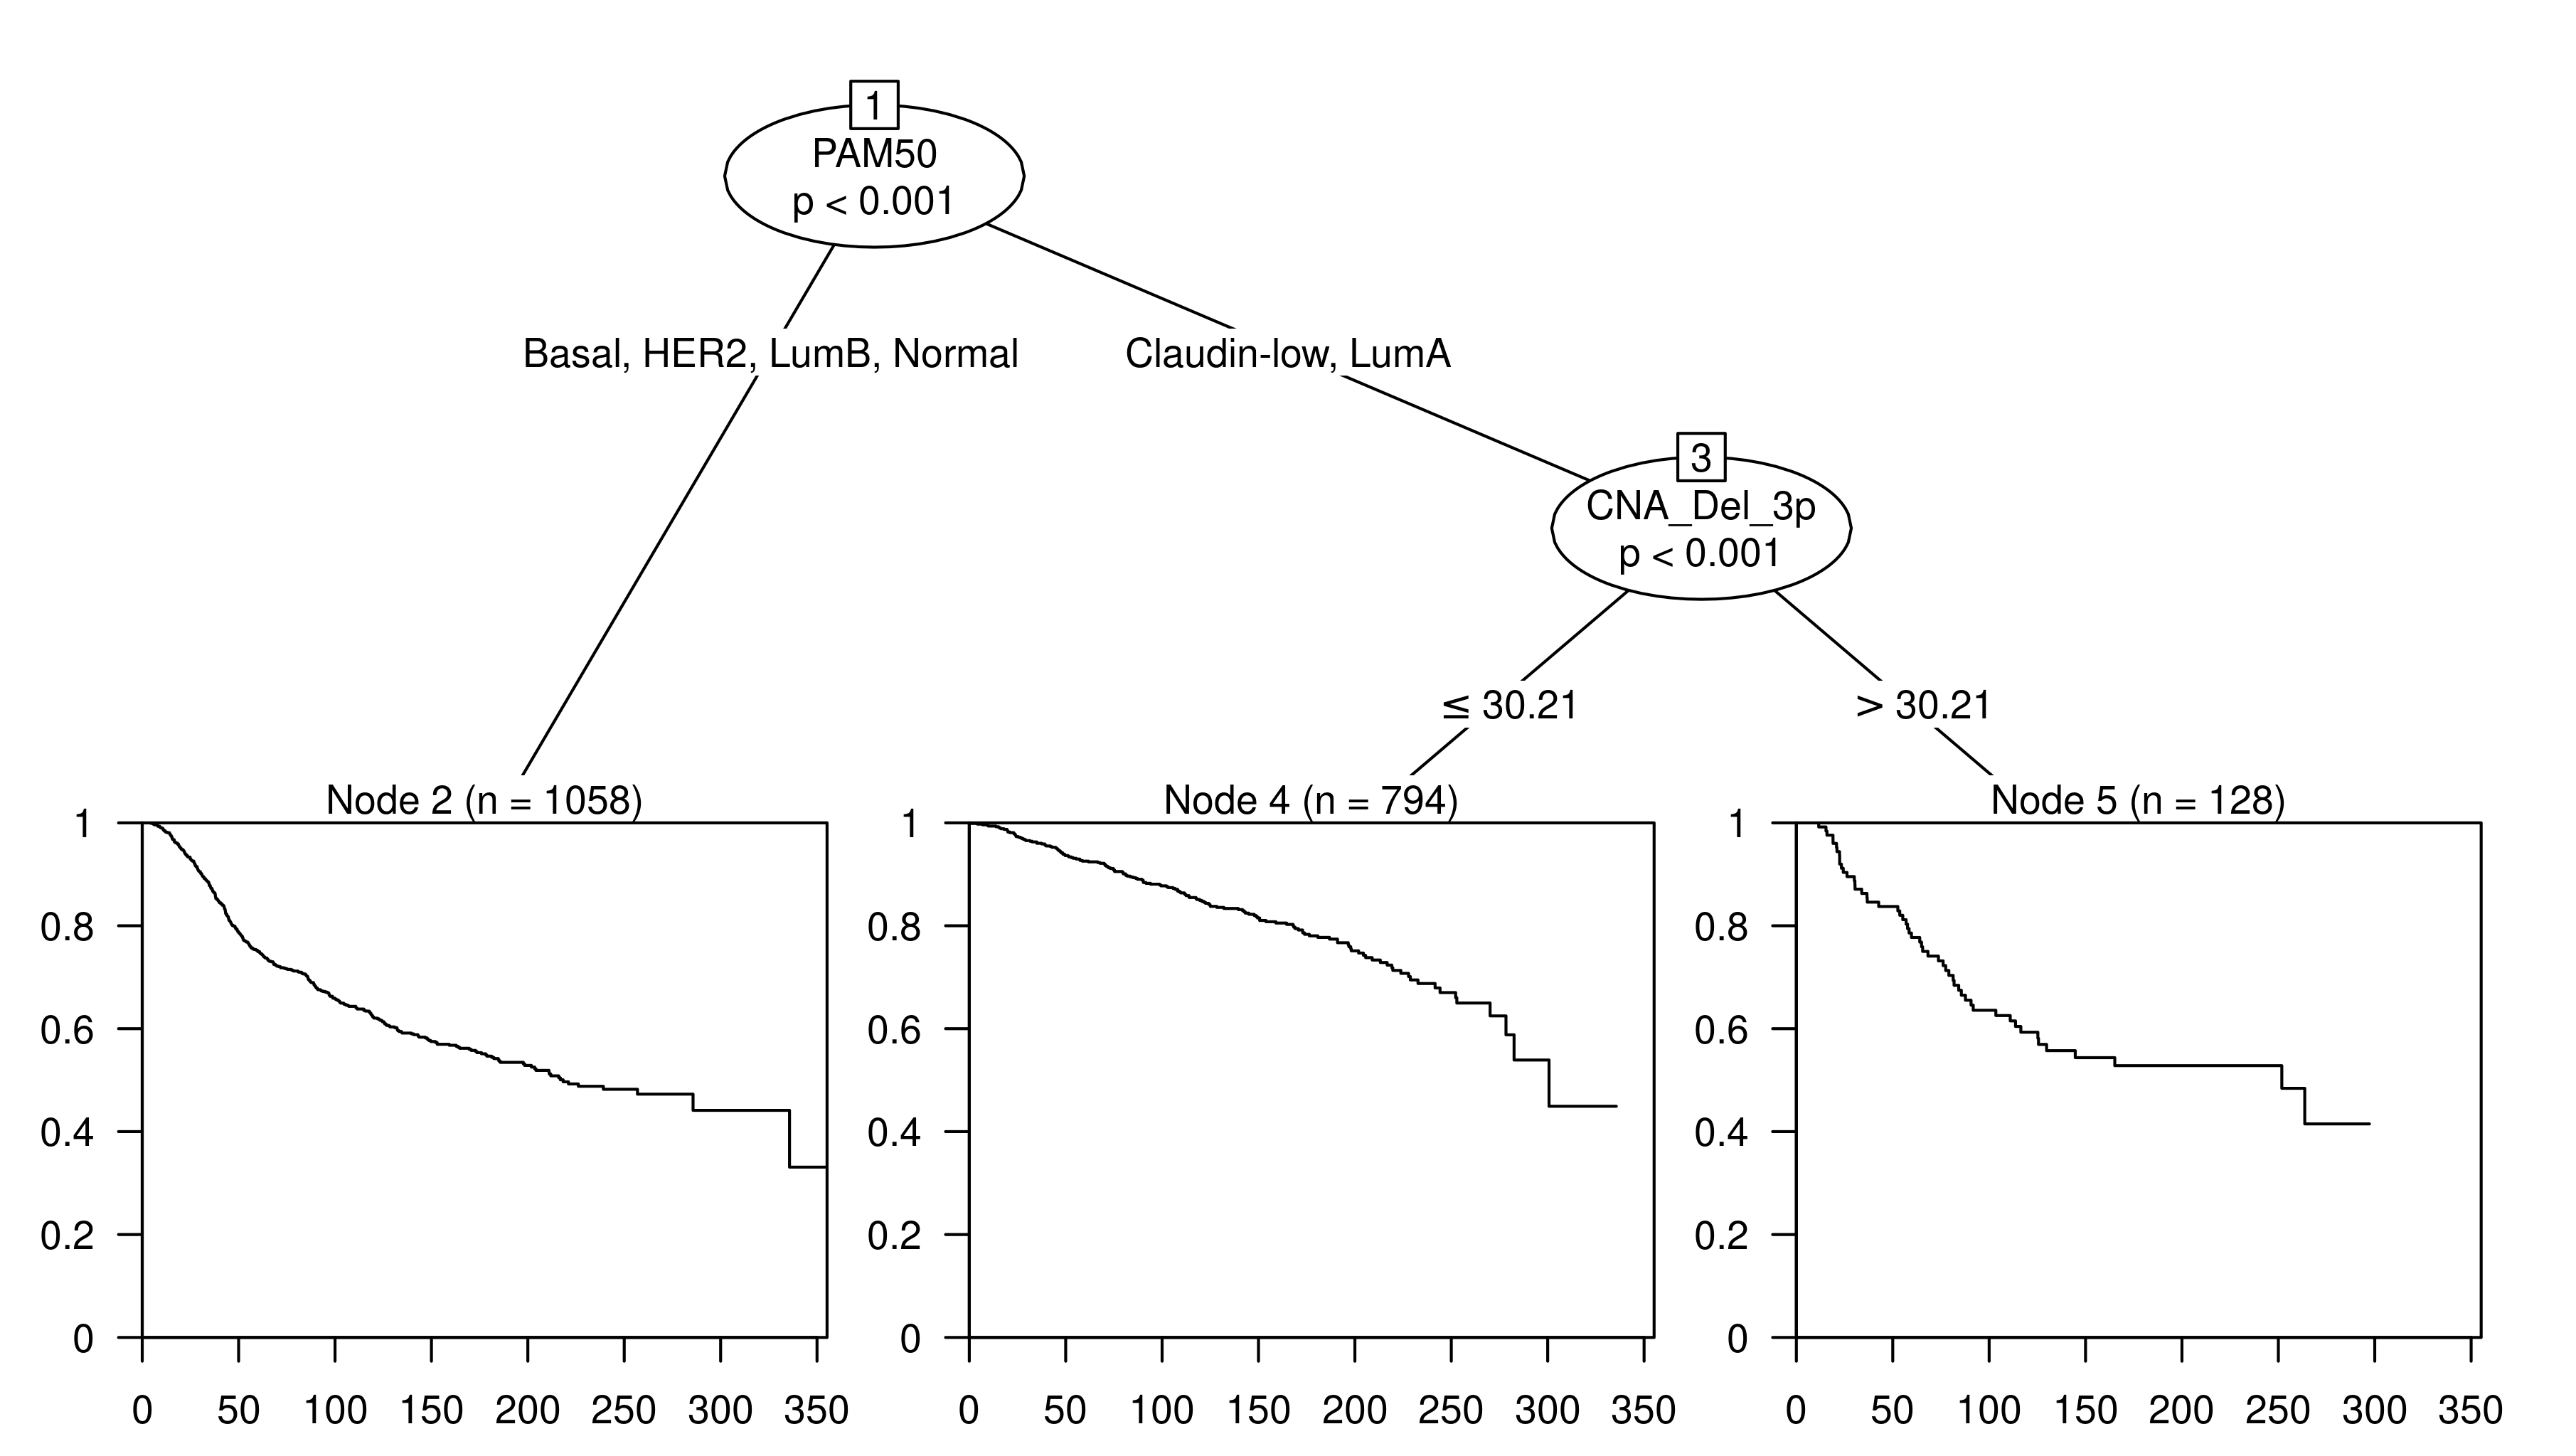
\includegraphics[width=1\textwidth]{../figures/Chapter_3/PA_Ctree_Survival_Burden_DSS_PAM50.png}

\vspace{0.5cm}

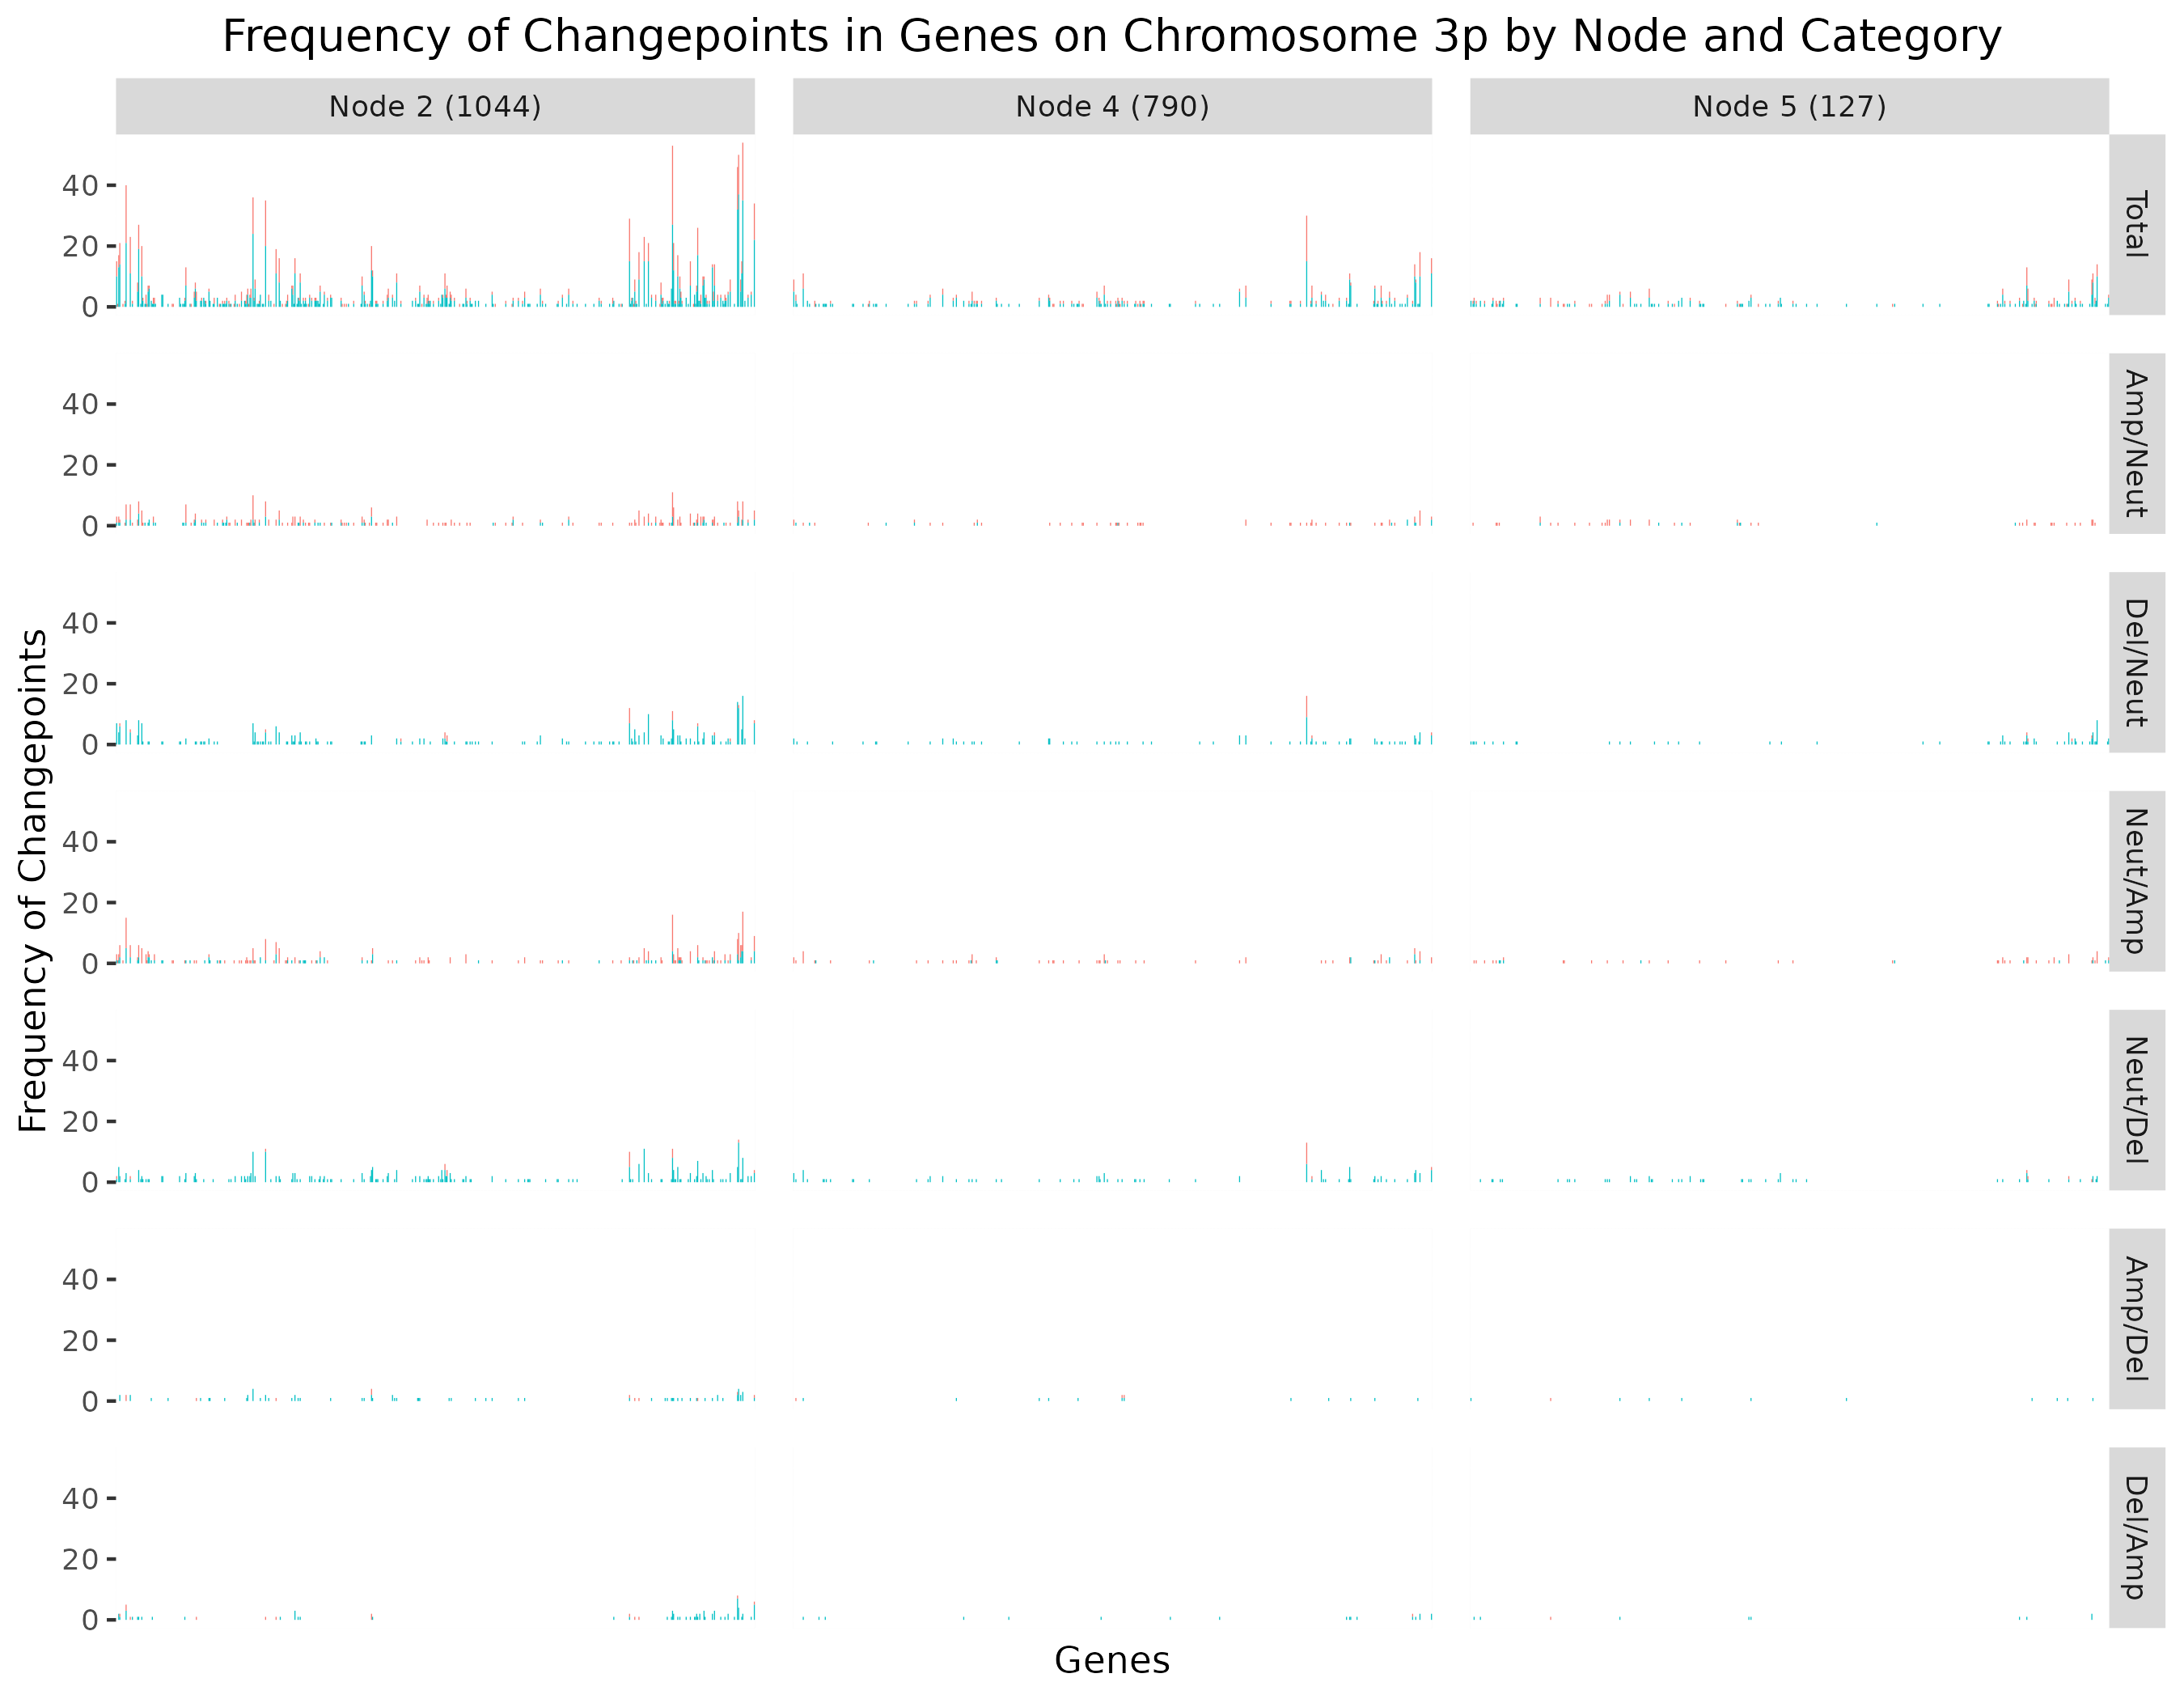
\includegraphics[width = 1\textwidth]{../figures/Chapter_6/Chromosome_3p_Barplot_Node.png}
\caption[Frequency of changepoints in genes across chromosome 3p, split by Node and Category, and coloured by allele.]{Frequency of changepoints in genes across chromosome 3p, split by Node and Category, and coloured by allele. For patients stratified into distinct survival patterns, Nodes 2, 4, and 5 corresponding to Figure \ref{fig:PAM50_PA_CNA_Burden_DSS} (figure panel columns), and for each changepoint category (panel rows), the frequency of that changepoint, observed in the each gene across chromosome 3p (x-axis) is plotted. Frequencies of the Major allele are coloured pink and the Minor allele coloured blue.}
\label{fig:Barplot_3p}
\end{figure}

\noindent CADM2, displaying 54 changepoints (Table \ref{tbl:Chr3p_Freq}). Node 4 and Node 5, comprising 790 and 127 patients, also display low numbers of changepoints. The gene with the highest frequencies of changepoints in Nodes 4 and 5 are SFMBT1 with 30 changepoints, and CADM2 with 14 changepoints. While it appears that some genes are more susceptible to containing a changepoint, there seems to be no characteristic changepoint pattern that distinguishes patients within nodes.

\begin{table}[!htb]
\caption[Top 10 genes on chromosome 3p with highest frequency of changepoints for patients in Nodes 2, 4 and 5.]{Top 10 genes on chromosome 3p with highest frequency of changepoints for patients in (A) Node 2, (B) Node 4, and (C) Node 5.}

\centering
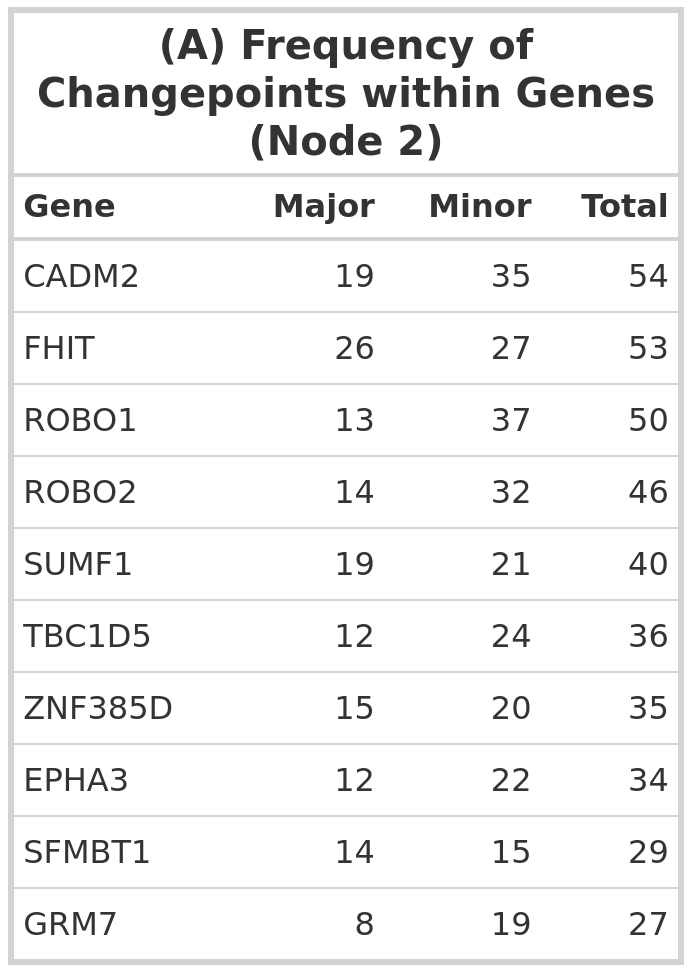
\includegraphics[width = 0.3\textwidth]{../tables/Chapter_6/Chr3_Node_2.png}
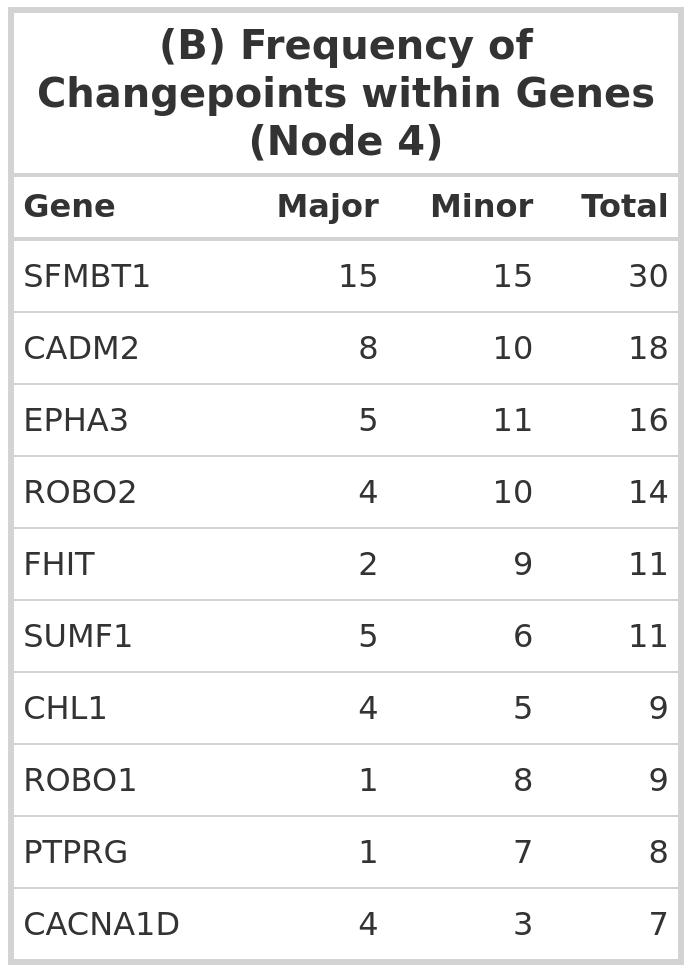
\includegraphics[width = 0.3\textwidth]{../tables/Chapter_6/Chr3_Node_4.png}
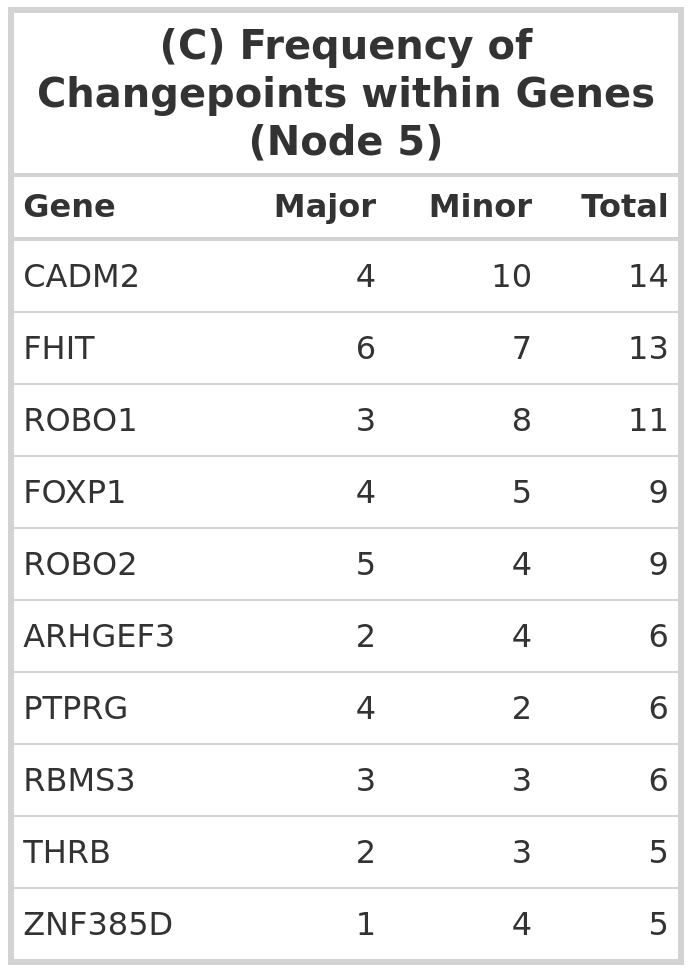
\includegraphics[width = 0.3\textwidth]{../tables/Chapter_6/Chr3_Node_5.png}
\vspace{1cm}
\label{tbl:Chr3p_Freq}
\end{table}

Chromosome 18q (Appendix F) and 11p (Figure \ref{fig:Barplot_11p}) also indicate low frequencies of changepoints within genes across the chromosome arms. Figure \ref{fig:Barplot_11p} displays a prominent peak in Node 3, count 113, and Node 7, count 161, corresponding to the gene TRIM5. 

\begin{figure}[!htp]
\centering

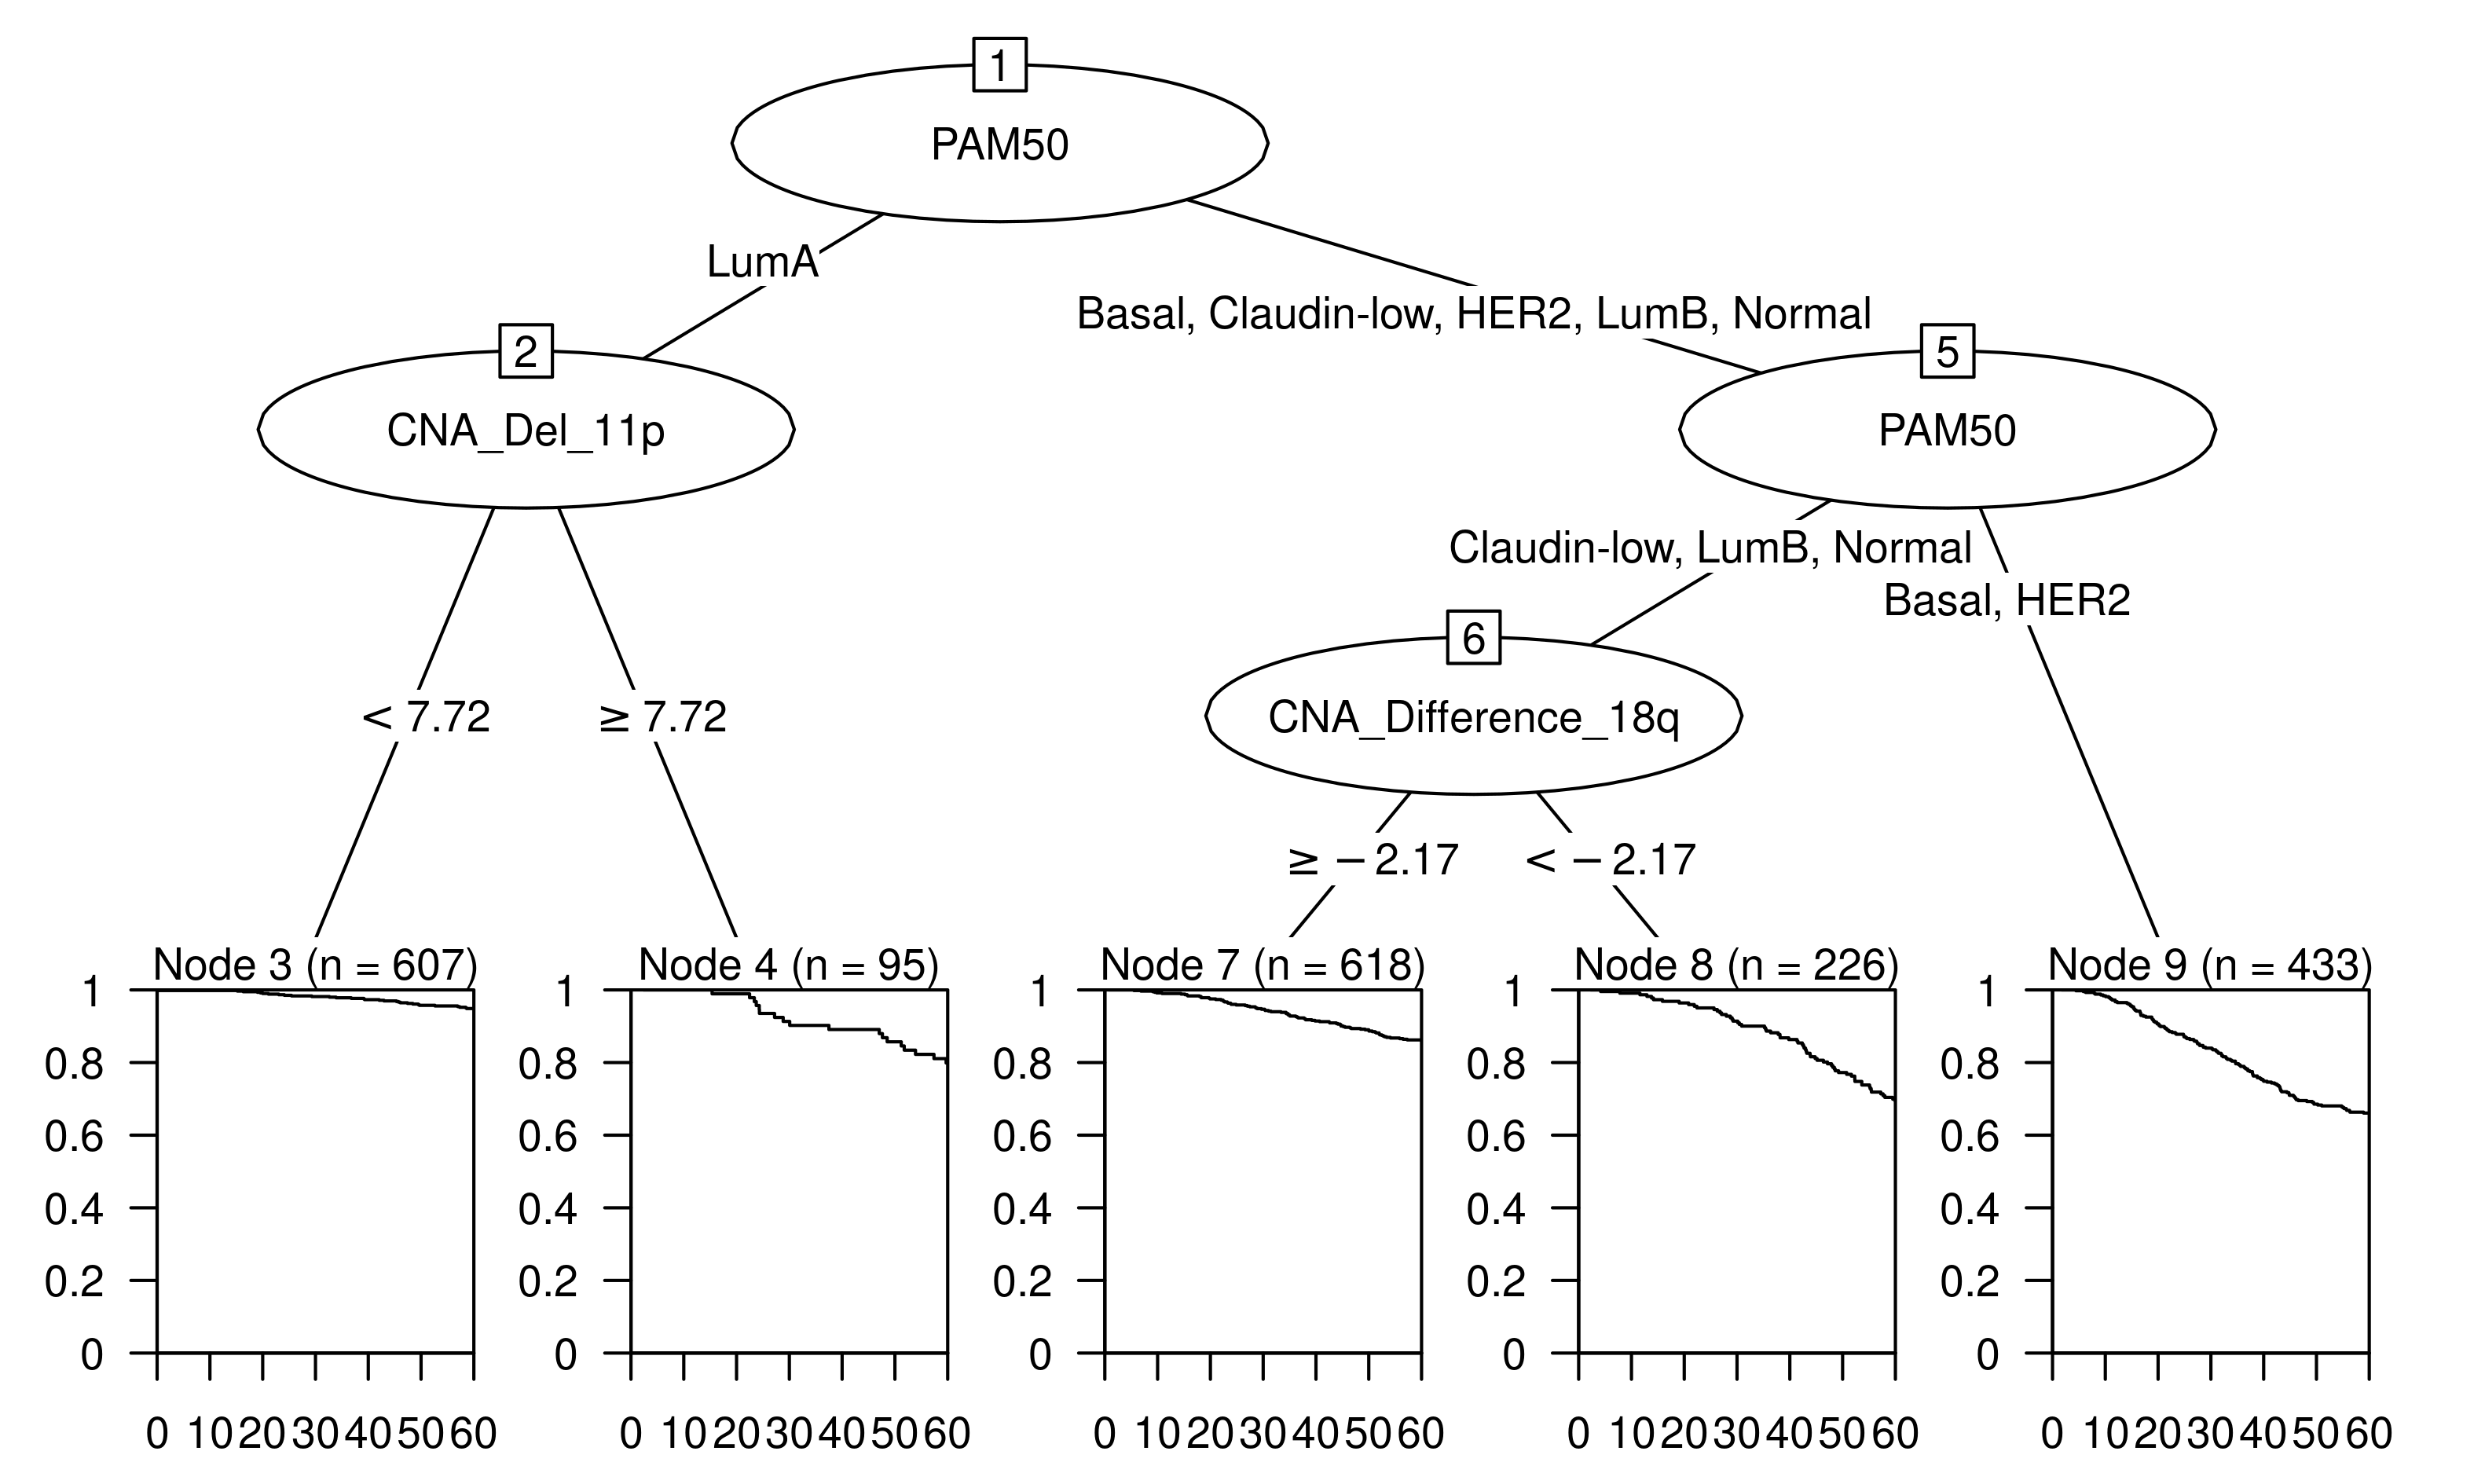
\includegraphics[width=1\textwidth]{../figures/Chapter_3/PA_PartyKit_Survival_Burden_FiveYearDSS_PAM50.png}

\vspace{0.5cm}

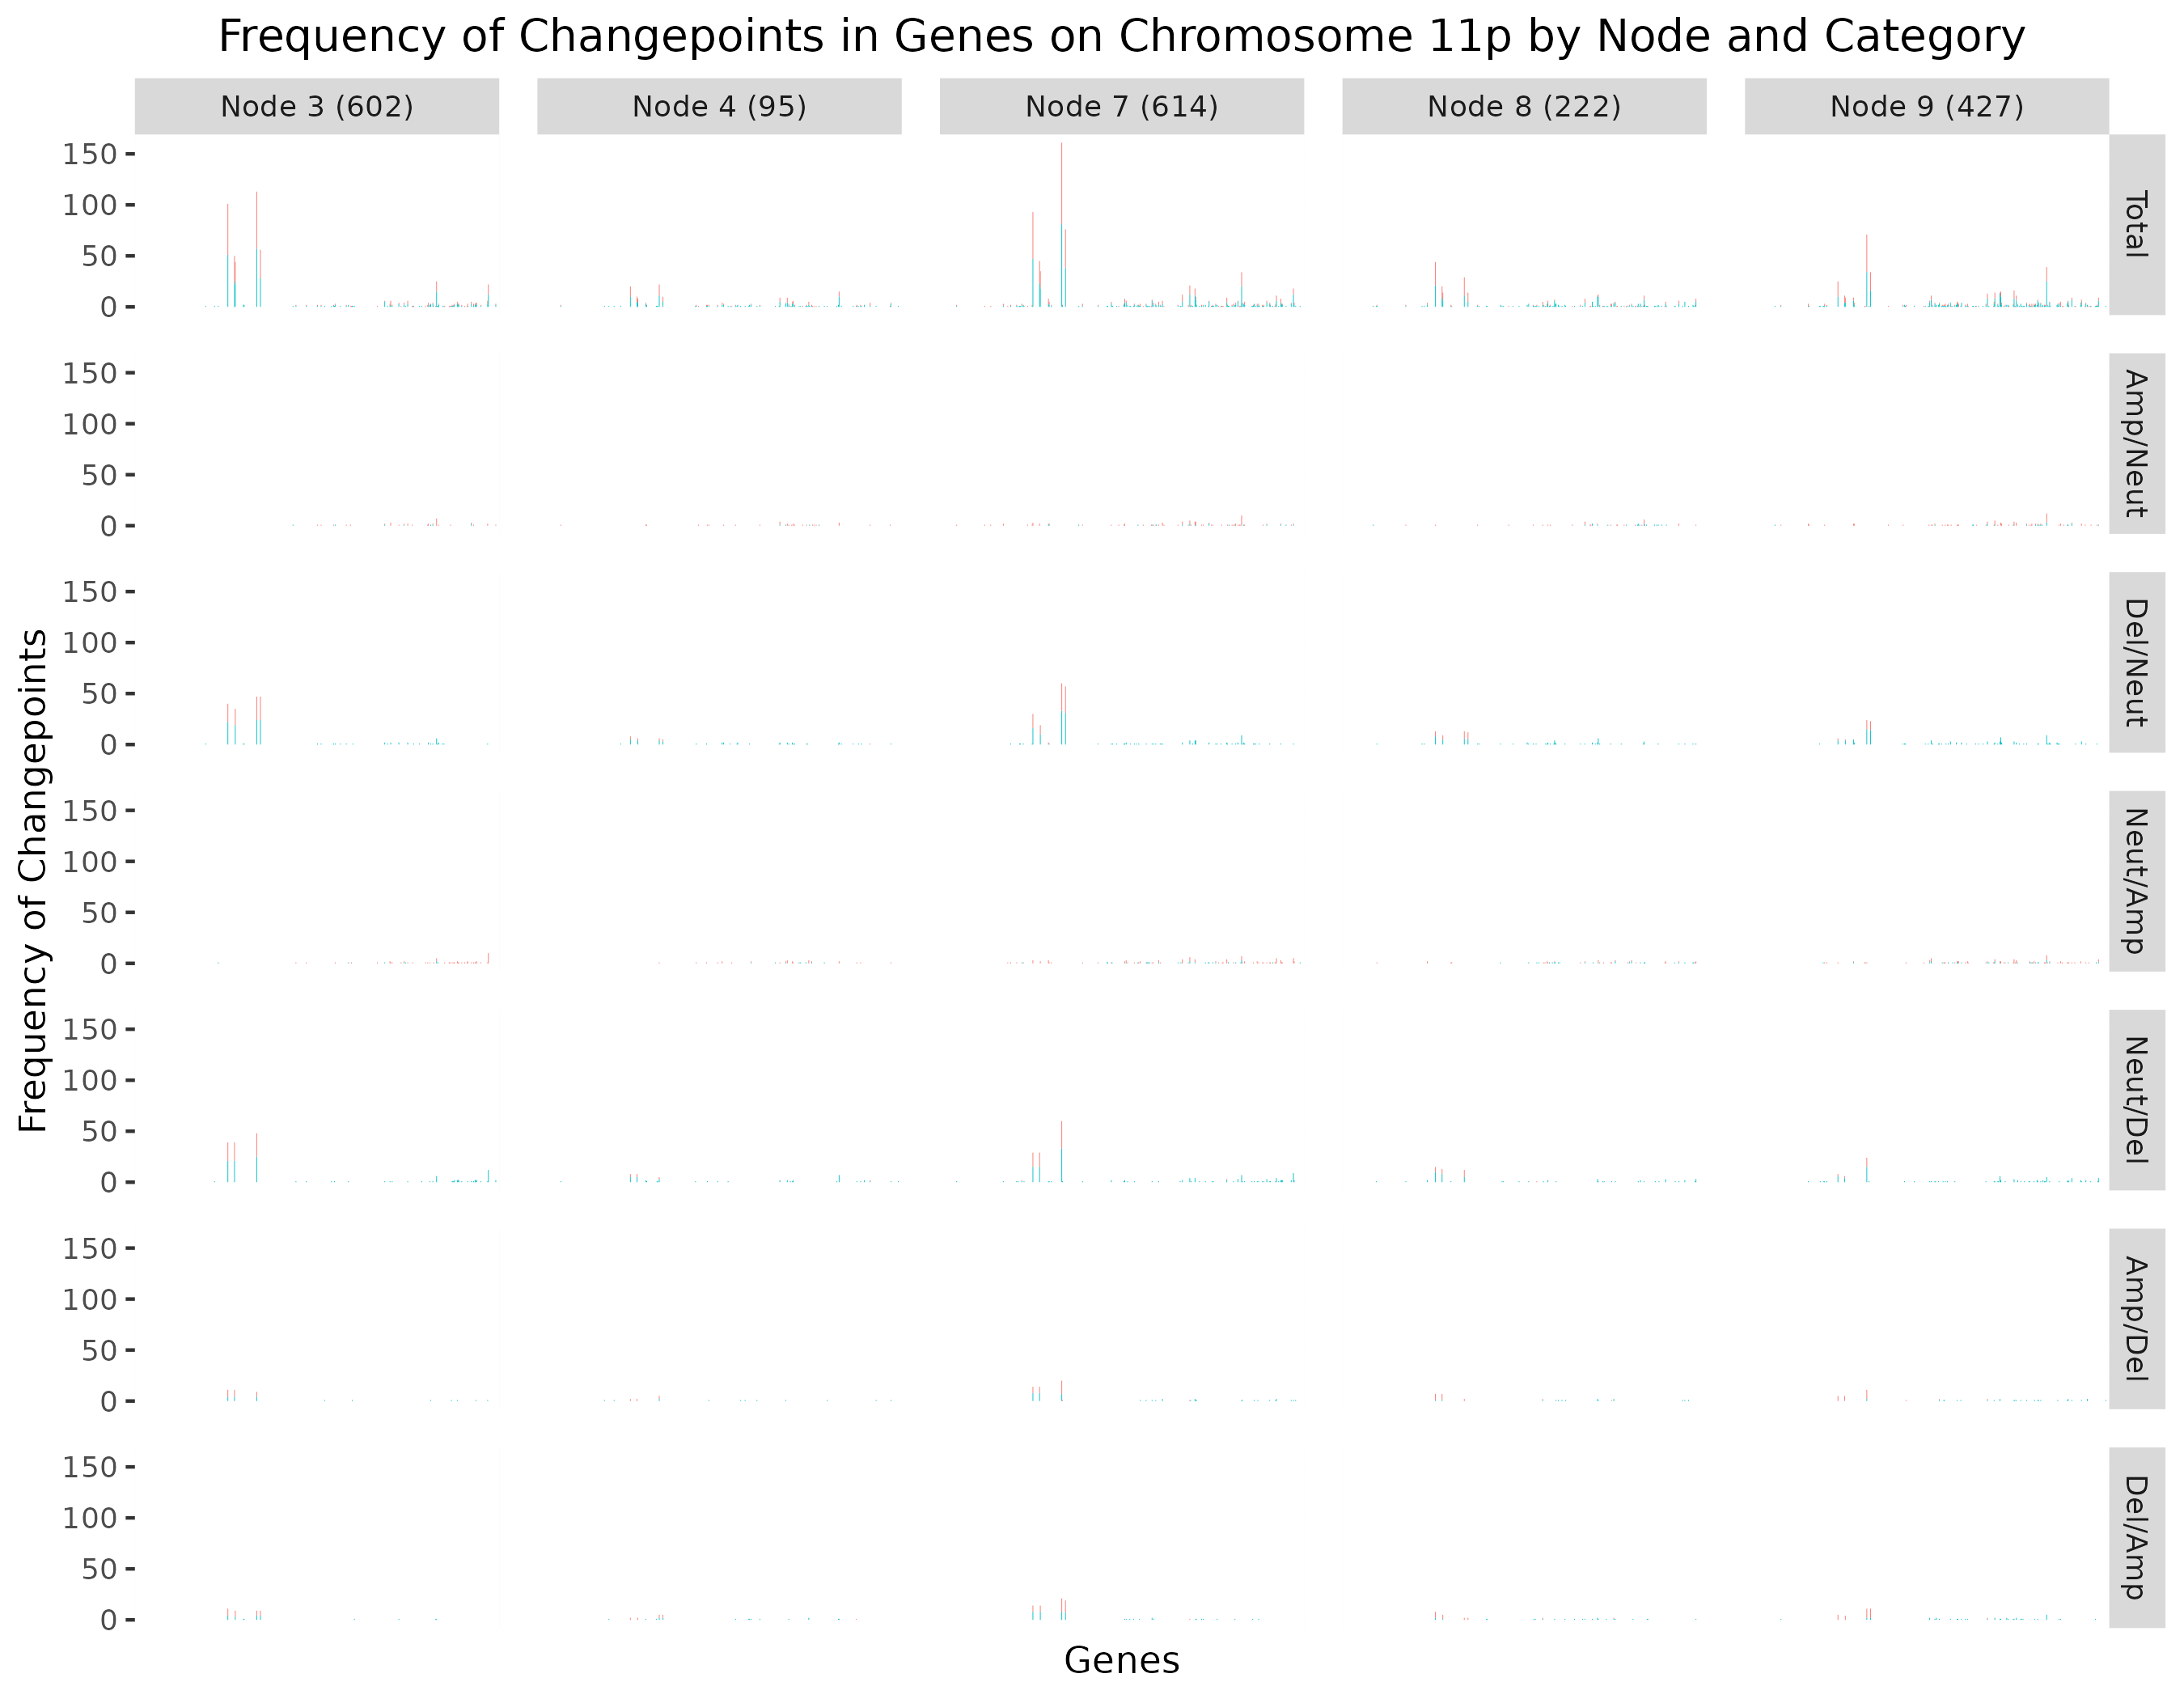
\includegraphics[width = 1\textwidth]{../figures/Chapter_6/Chromosome_11p_Barplot_Node.png}
\caption[Frequency of changepoints in genes across chromosome 11p, split by Node and Category, and coloured by allele.]{Frequency of changepoints in genes across chromosome 11p, split by Node and Category, and coloured by allele. For patients stratified into distinct survival patterns, Nodes 3, 4, 7, 8 and 9, corresponding to Figure \ref{fig:PAM50_PA_CNA_Burden_FiveYearDSS} (figure panel columns), and for each changepoint category (panel rows), the frequency of that changepoint, observed in the each gene across chromosome 11p (x-axis) is plotted. Frequencies of the Major allele are coloured pink and the Minor allele coloured blue.}
\label{fig:Barplot_11p}
\end{figure}

These results indicate that while a large number of genes on chromosomes 3p, 18q and 11p, in subsets of patients, are affected by amplifications or deletions, as seen in Figure \ref{fig:heatmap_Both} where a large number patients display widespread amplifications and/or deletions, the changepoints are generally not occurring in the genes (Figures \ref{fig:Barplot_3p} and \ref{fig:Barplot_11p} and Tables \ref{tbl:Chr3p_Freq} and \ref{tab:Chr3p_11p}). The distribution of changepoints across all genes annotated in the CNA data, for which genomic location information could be obtained, is provided in Figure \ref{fig:Barplot_Total}, again indicating that apart from a few genes harbouring large numbers of changepoints, changepoints are not frequently observed in genes. Genes displaying high numbers of changepoints include TRIM5 on chromosome 11, LCE1E on chromosome 1 and OPHN1 on the X chromosome, with 400 (204 on Major allele and 196 on Minor allele), 328 (188 on Major allele and 140 on Minor allele), and 289 (121 on Major allele and 168 on Minor allele) changepoints observed across all patients, where more than one changepoint can occur in a patient (Figure \ref{fig:Barplot_Total} and Table \ref{tab:Genes_Freq_Table}).

\begin{table}[!htb]
\caption[Top 10 genes on chromosome 11p with highest frequency of changepoints for patients in Nodes 3 and 7.]{Top 10 genes on chromosome 11p with highest frequency of changepoints for patients in (A) Node 3 and (B) Node 7.}
\centering
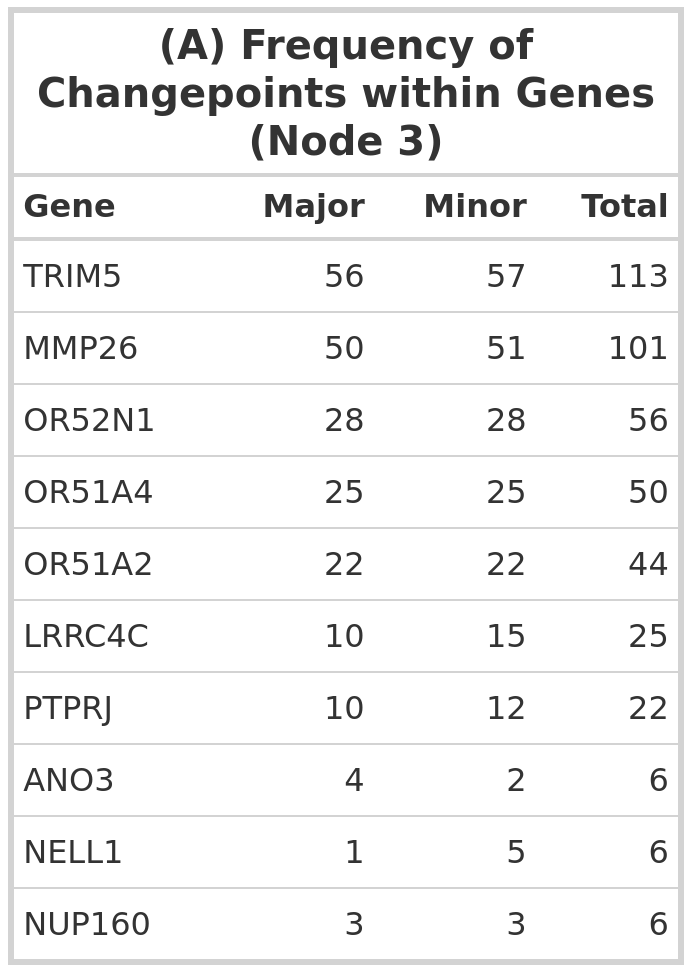
\includegraphics[width = 0.3\textwidth]{../tables/Chapter_6/Chr11_Node_3.png}
\hspace{1cm}
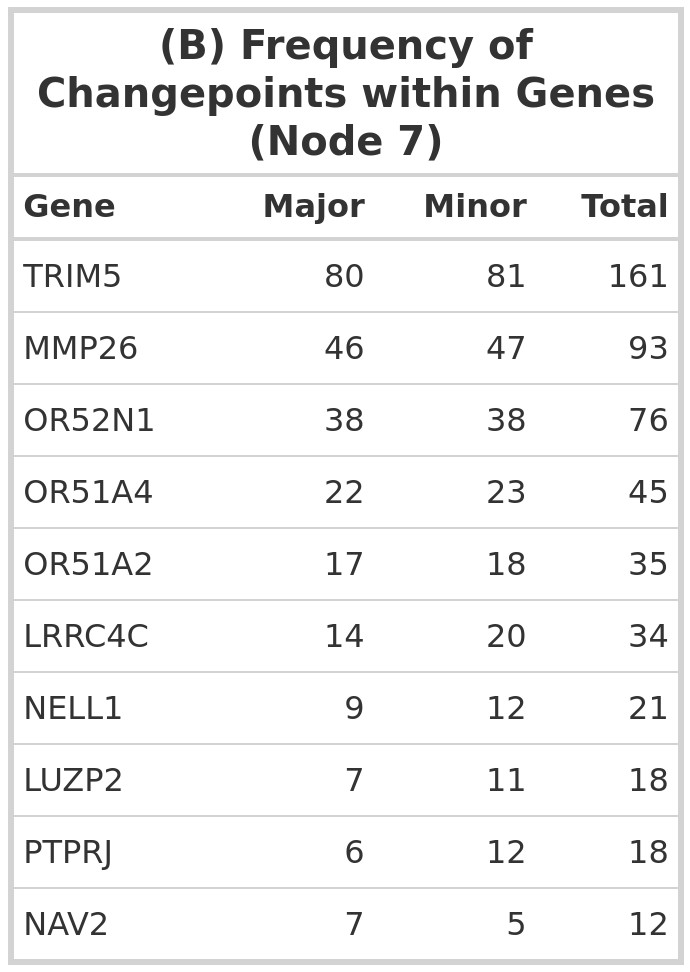
\includegraphics[width = 0.3\textwidth]{../tables/Chapter_6/Chr11_Node_7.png}
\label{tab:Chr3p_11p}
\end{table}

\begin{table}[!htb]
\caption[Frequency of changepoints within genes, the top 20 genes are shown.]{Frequency of changepoints within genes, the top 20 genes are shown.}
\centering
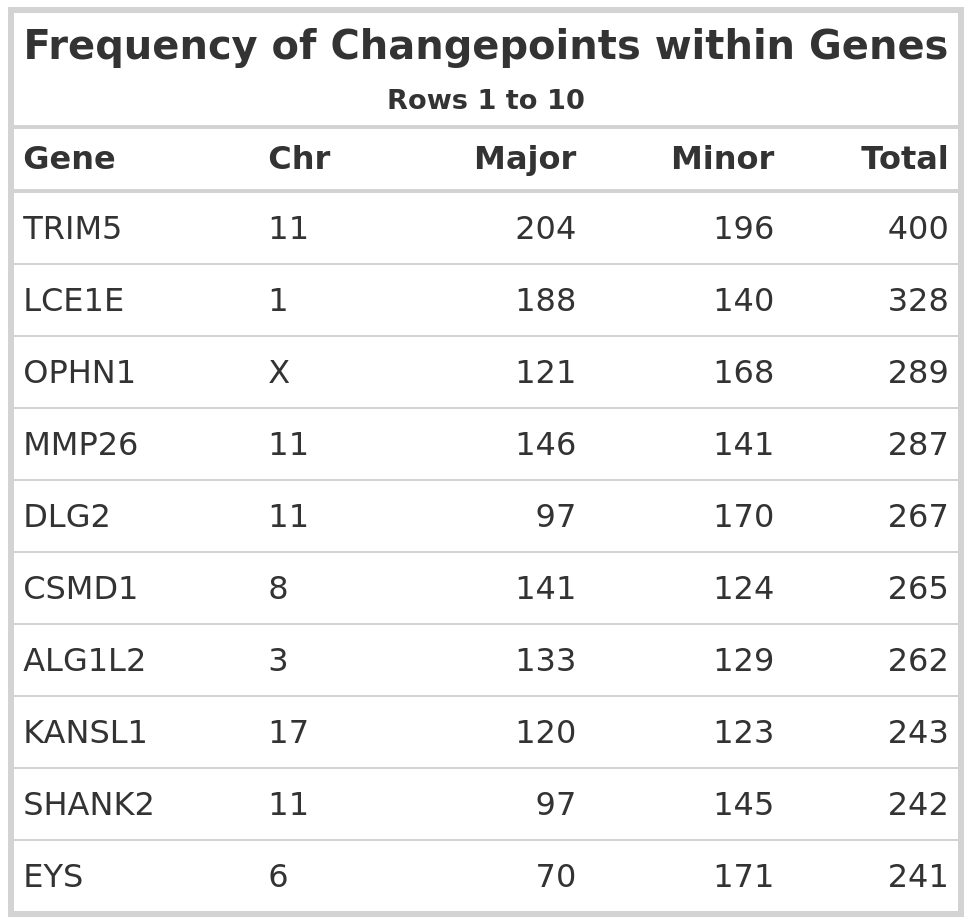
\includegraphics[width = 0.48\textwidth]{../tables/Chapter_6/Gene_Table_Freq_1.png}
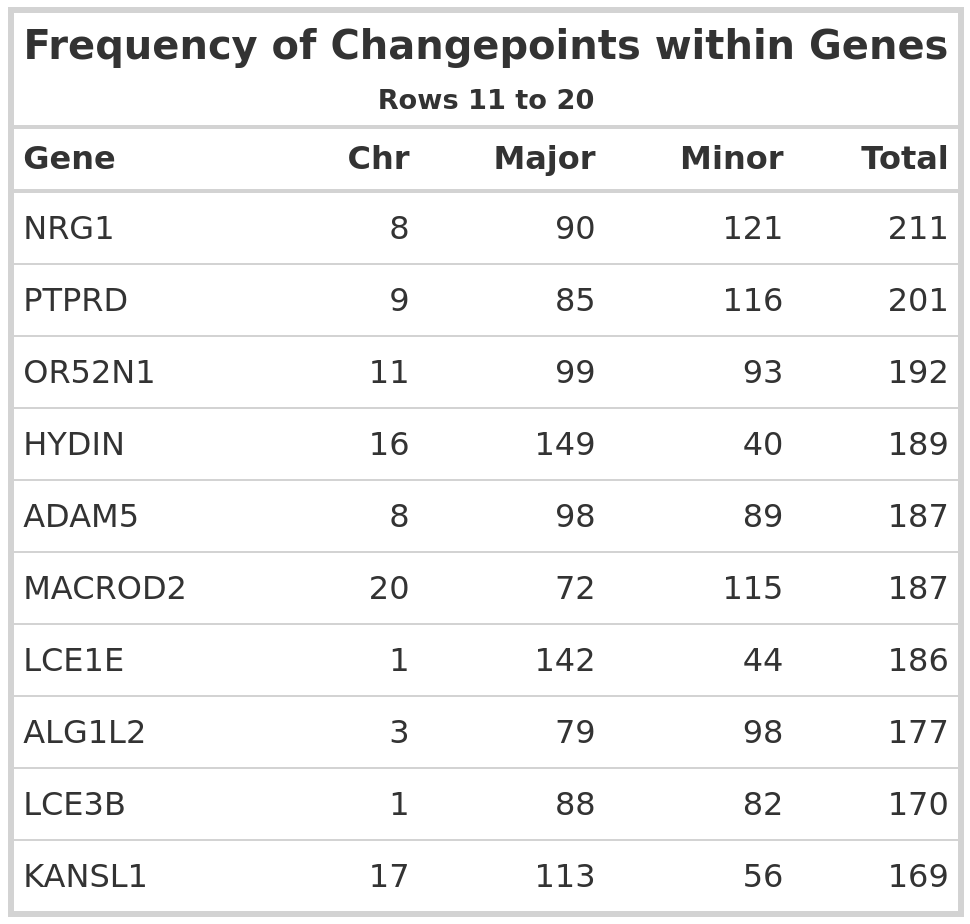
\includegraphics[width = 0.48\textwidth]{../tables/Chapter_6/Gene_Table_Freq_2.png}
\label{tab:Genes_Freq_Table}
\end{table}  

While Figure \ref{fig:Barplot_Total} and Table \ref{tab:Genes_Freq_Table} indicate which genes most frequently harbour changepoints, no indication is given regarding how much of the surrounding genome is of altered copy number, i.e. the number of bases affected by an amplification or deletion. To detect changepoints, based on the $TS$ and $TE$ lengths, we apply the ADIM to each gene. 

Notably, different genes have different base lengths, meaning that in the gene-centric approach the observed interval $d$ will have variable lengths. Consequently, genes of larger length may display higher frequencies of changepoints, while genes of shorter length may display low numbers of changepoints. In addition, not all categories of changepoints may occur within $d$ and observation of small numbers of changepoints within $d$ may not support model fitting.

Out of 22,544 genes considered, 10,966 genes do not display any changepoint, meaning no model is fit for those genes. Fitting multivariate ADIM, using the \texttt{MCMCglmm()} function, is supported for only 2,290 genes. The 9,288 genes for which the \texttt{MCMCglmm()} function is not supported require the use of a stronger or proper prior to be implemented. 

We first test whether the mean lengths of the changepoint alterations, $TS$ and $TE$, are greater than 10kb, where significance is determined by the lower bound of the confidence interval for the relevant length, $TS$ or $TE$, being greater than 10kb, $LB > 10$kb. Figure \ref{fig:PerGene_MCMC}, the tile plot displaying the results from applying the ADIM to 2,290 genes, indicates the widespread presence of changepoints with $TS$ or $TE$ greater than 10kb. Significance in $TS$ but not $TE$ is indicated in purple, significance in $TE$ but not $TS$ is indicated in blue and significance in both is indicated in green. The number of observations in each category, for each gene, is provided by the diameter size of the point, larger points indicating larger sample size. For a large number of genes, the mean $TS$ for the Amp/Neut and Del/Neut categories, the mean $TE$ for the Neut/Amp and Neut/Del categories, and the mean $TS$ or $TE$ for the Del/Amp and Amp/Del categories are significantly greater than 10kb, $LB > 10$kb. We also observe that deletion events, i.e. Neut/Del, Del/Neut, Amp/Del and Del/Amp, occur more often on the Minor allele than on the Major allele. A number of chromosomes, including chromosome 1, 3, 8, 16, 17 and 23, contain genes harbouring a large number of changepoints with $TS$ or $TE$ length greater than 10kb.

Next we test whether the mean lengths for each changepoint category ($TS$ or $TE$) are greater than 10,000kb, significance determined by the lower bound of the confidence interval for the relevant $TS$/$TE$ length being greater than 10,000kb, $LB > 10,000$kb (Figure \ref{fig:PerGene_10000_MCMC}). Chromosomes containing genes with changepoints of significant length, at larger sample sizes, include chromosomes 1, 6, 8, 11 and X.

Table \ref{tab:TopLength_Genes_1}A indicates which genes harbour changepoints with a $TS$ and/or $TE$ $>10,000$kb on average, with a within category sample size greater than 30 observations. Noteworthy genes identified include OR52N1 on chromosome 11, TRIM5 on chromosome 11, and ALG1L2 on chromosome 3, all containing a significant Del/Amp on the Major allele. The gene with the largest number of changepoints, with average $TS$ and/or $TE$ length $>10,000$kb, is LCE1E with $n = 142$. 

As the \texttt{MCMCglmm()} function did not support model fitting for 9,288 genes, univariate ADIM fitted using the \texttt{lm()} function is applied, producing model estimates for all 22,544 genes.

Testing whether the mean lengths of the changepoint alterations, $TS$ and $TE$, are greater than 10kb, $LB > 10$kb, and whether the mean lengths of the changepoint alterations, $TS$ and $TE$, are greater than 10,000kb, $LB > 10,000$kb (Figures \ref{fig:PerGene_LM} and \ref{fig:PerGene_10000_LM}) produces similar results for the 2,290 genes considered previously, but also provides information on an additional 9,288 genes, highlighting additional genes with significant changepoints, one of which is observed on chromosome 1, where a Del/Amp changepoint on the Major allele is observed. Table \ref{tab:TopLength_Genes_1}B indicates which genes harbour changepoints with a $TS$ and/or $TE$ $>10,000$kb on average, with a within category sample size greater than 30 observations, fitted using the \texttt{lm()} function. The only difference observed between the results produced using \texttt{lm()} (Table \ref{tab:TopLength_Genes_1}A) and \texttt{MCMCglmm()} (Table \ref{tab:TopLength_Genes_1}B) is the inclusion of LCE3B, a gene where the MCMCglmm model did not support fitting (Table \ref{tab:TopLength_Genes_1}A). Chromosomes containing genes of interest include chromosome 1, 3, 6, 8, 9, 10, 11, 20 and X.

Exploring further the identified point of focus, Del/Amp changepoint on the Major allele in gene OR52N1, KM survival curves for DSS outcome are produced and compared for patients who exhibit or do not exhibit this particular changepoint profile (Figure \ref{fig:TopLength_Genes_Surv}A). Similarly, DSS KM survival curves are produced, for two further points of focus, Del/Amp changepoint on the Major allele in gene TRIM5 (Figure \ref{fig:TopLength_Genes_Surv}B) and Del/Amp changepoint in gene ALG1L2 (Figure \ref{fig:TopLength_Genes_Surv}C). Applying the log-rank test for each point of focus indicates patients with a Del/Amp changepoint in ALG1L2 have worse DSS outcomes than patients that do not exhibit that changepoint, $p = 0.03$. However, when multiple testing correction is applied, this p-value becomes non-significant at $\alpha = 0.05$. 

\begin{figure}[H]
\centering

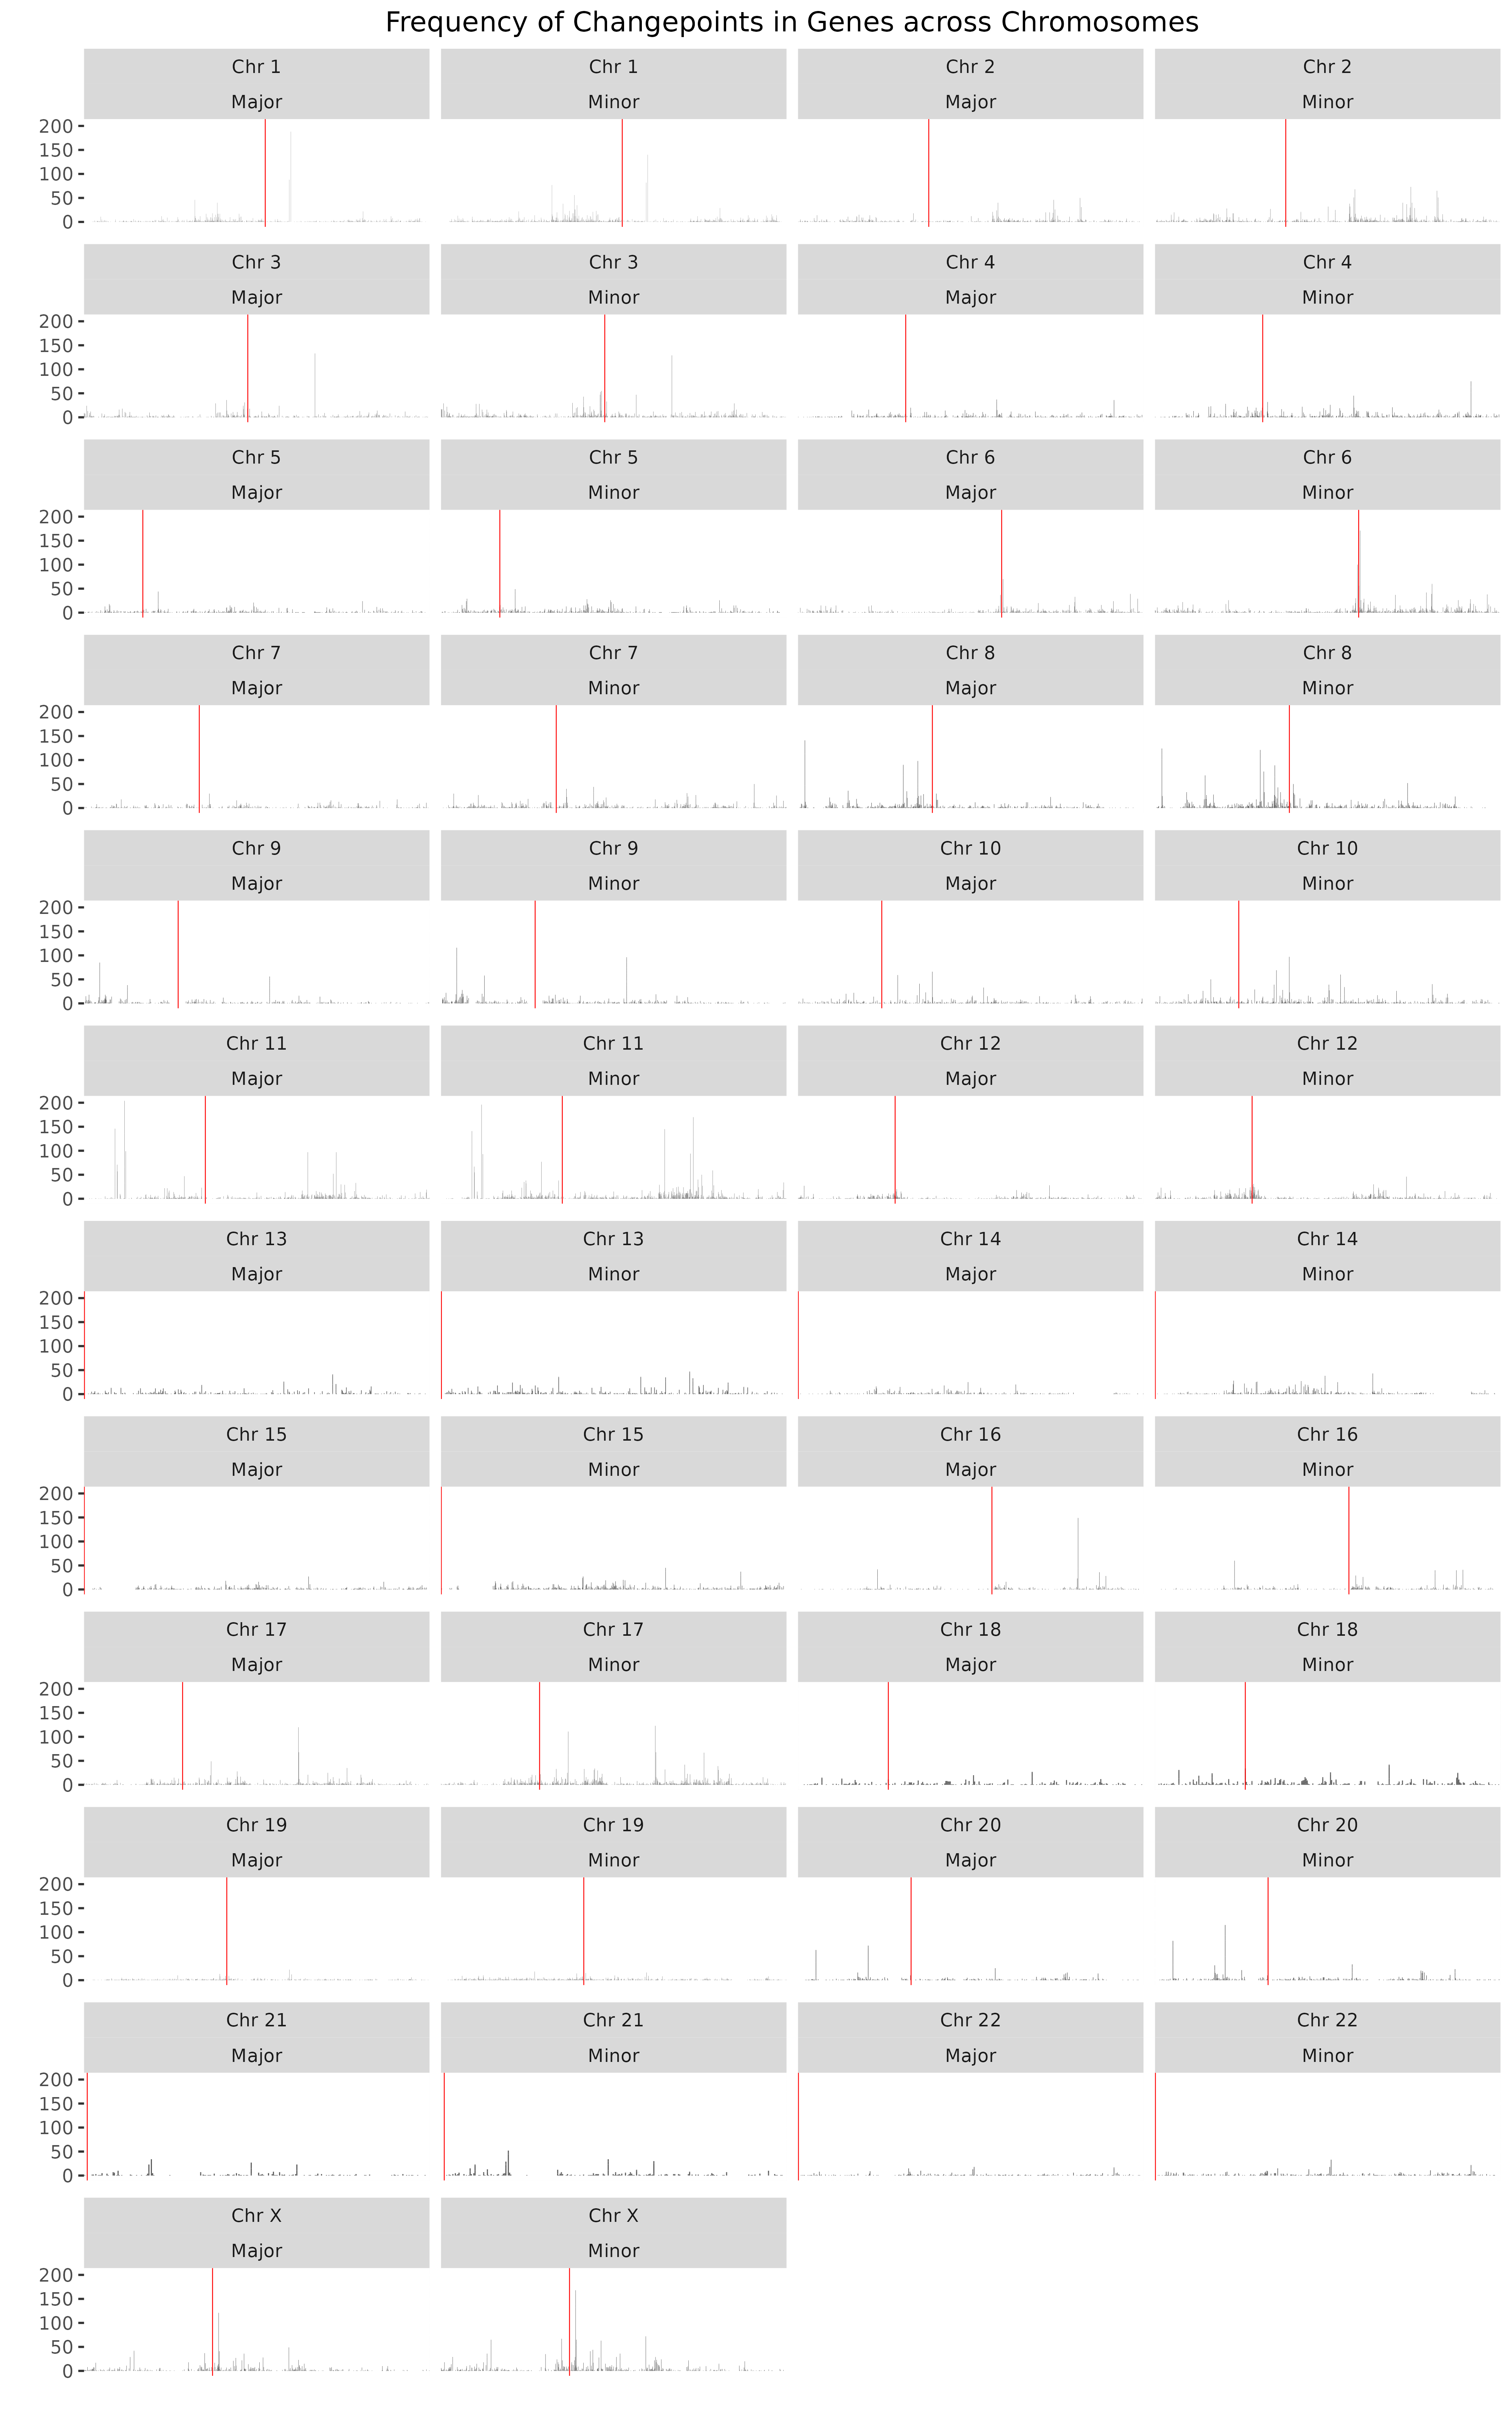
\includegraphics[width = 1\textwidth, height = 23cm]{../figures/Chapter_6/All_Genes_Barplot.png}

\caption[Frequency of changepoints in genes across each chromosome and allele.]{Frequency of changepoints in genes across each chromosome and allele. Scale of y-axis is the same across all chromosomes and the red line indicates the midpoint of the centromere.}
\label{fig:Barplot_Total}
\end{figure}

\begin{figure}[H]
\centering
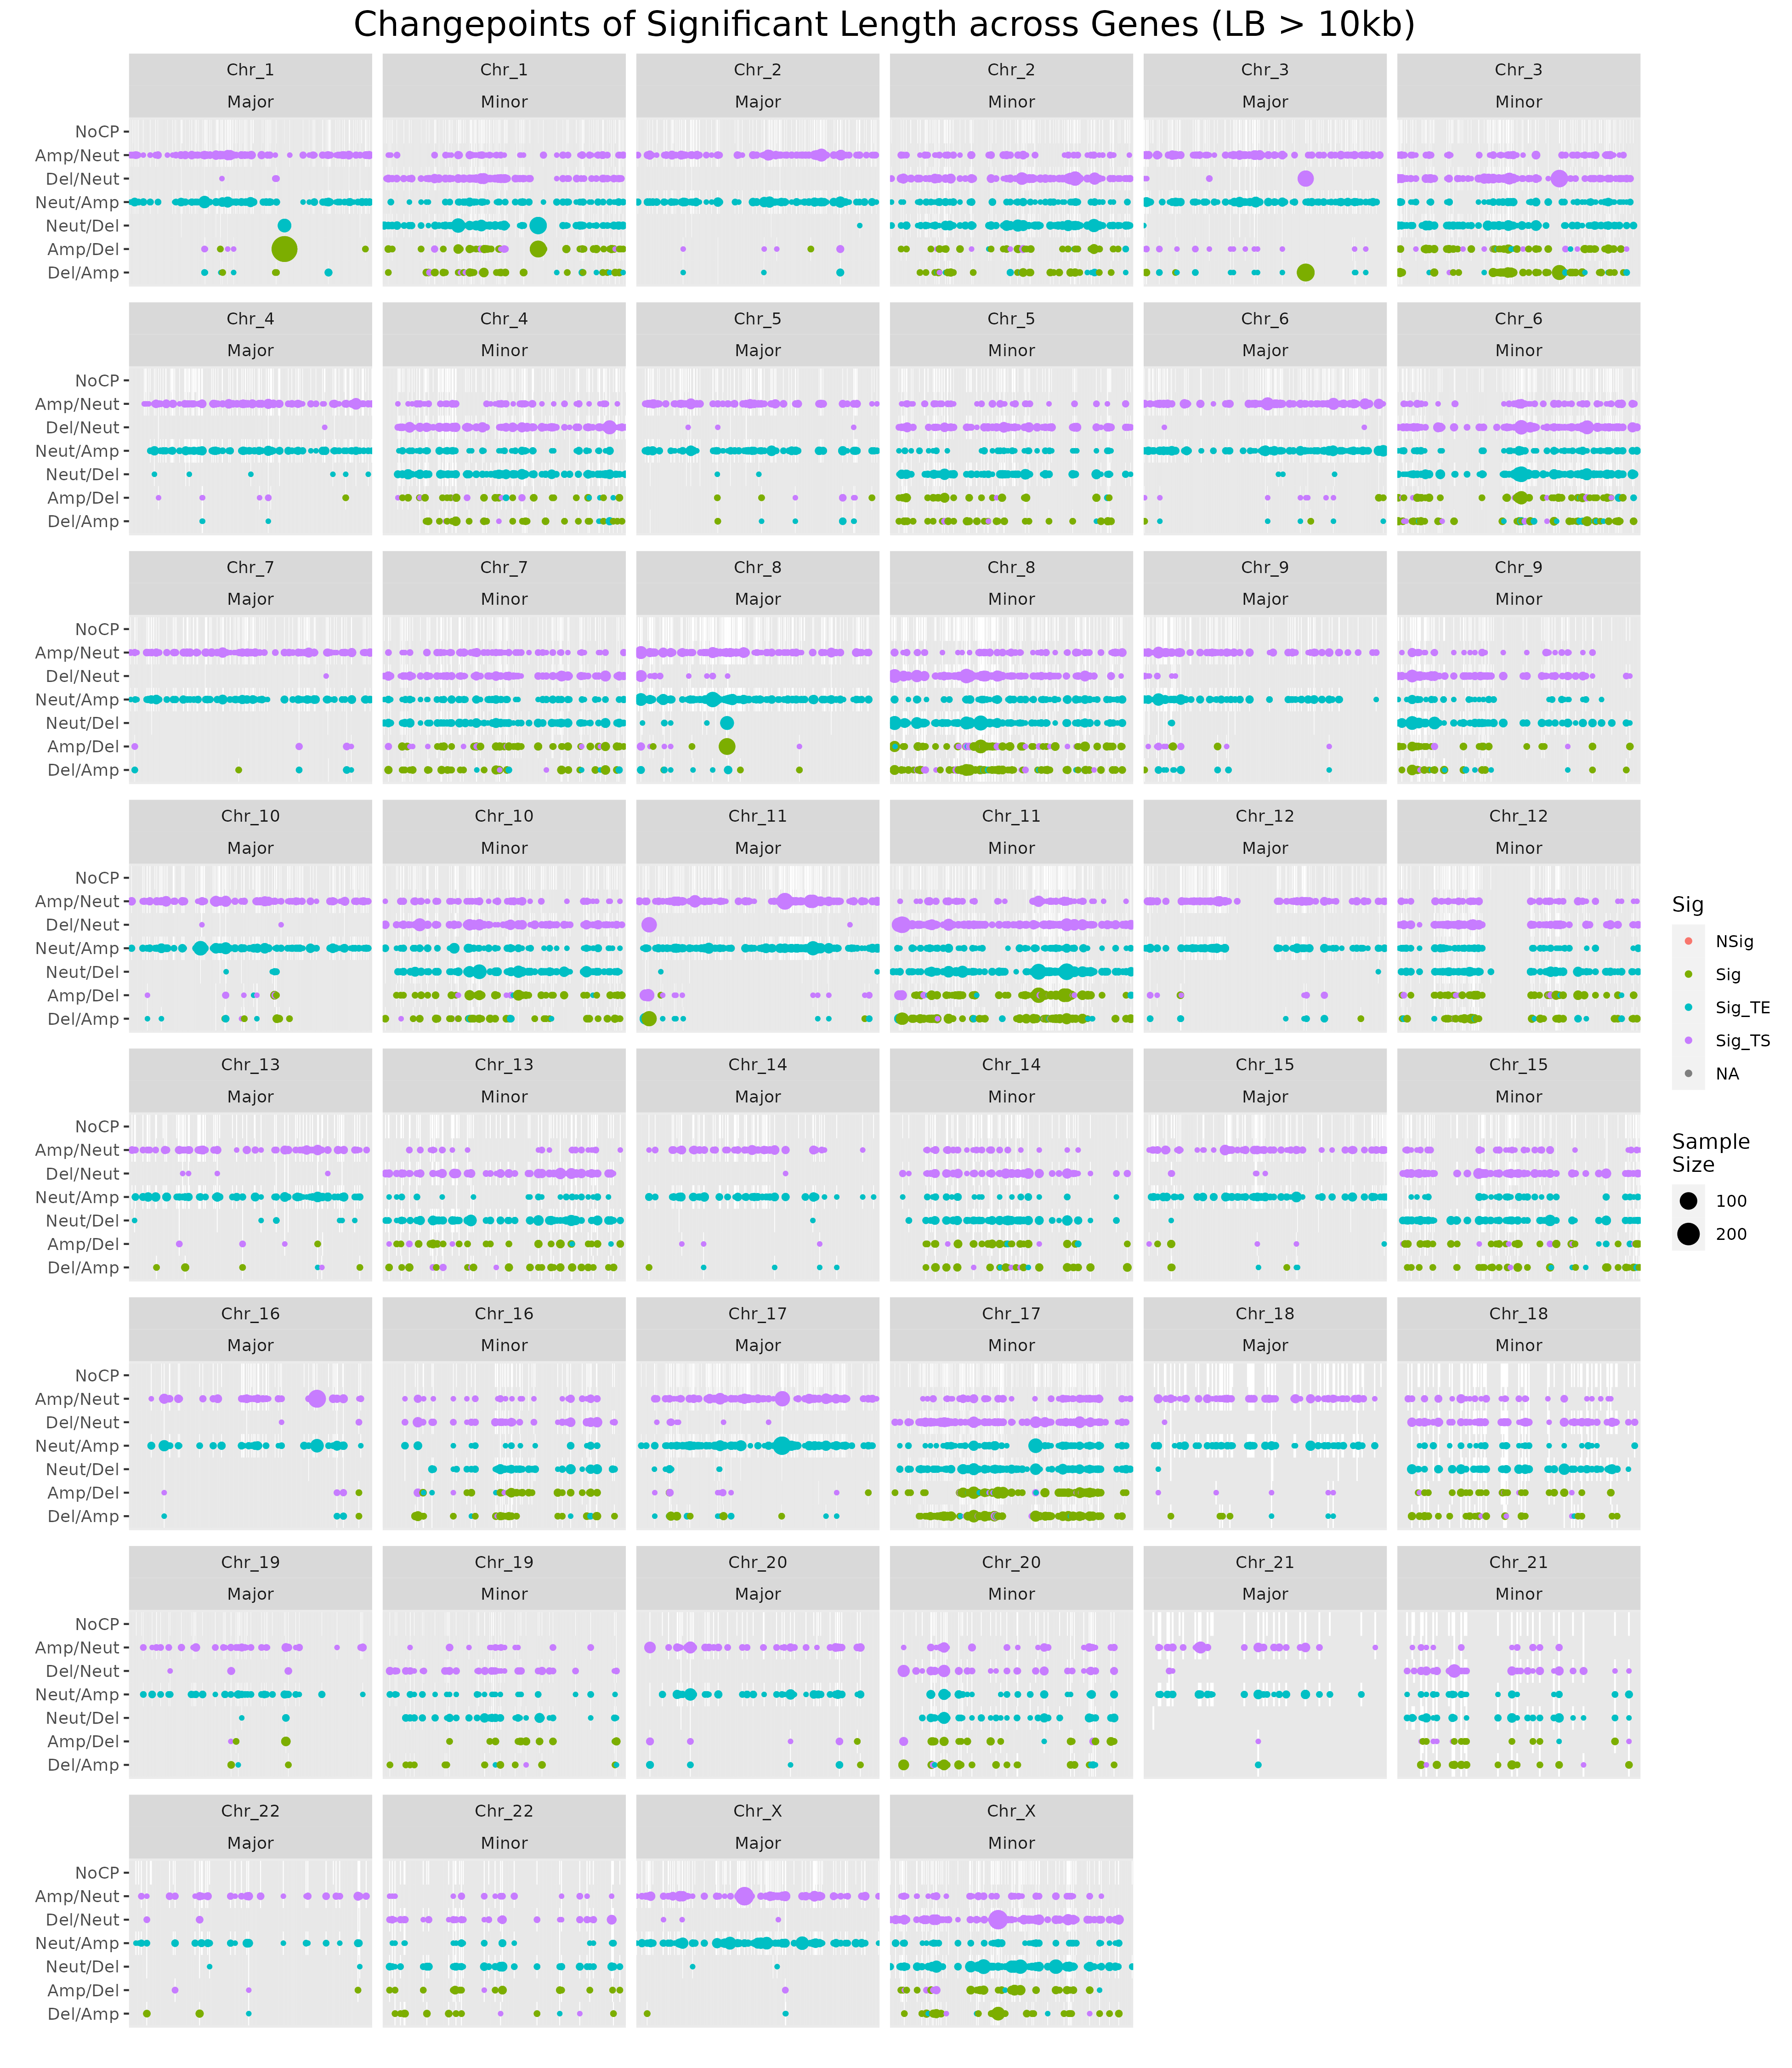
\includegraphics[width = 1\textwidth, height = 22cm]{../figures/Chapter_6/PerGene_MCMC_Zero_Thesis.png}
\caption[Application of multivariate Allele-Dependent Intercept Model to each gene ($LB > 10$kb).]{Application of multivariate Allele-Dependent Intercept Model to each gene, providing confidence intervals for each category and allele. Each panel, corresponding to chromosome and allele, displays significance of changepoint determined by $LB > 10$kb. NoCP corresponds to NoChangepoint. Fitted using the \texttt{MCMCglmm()} function.}
\label{fig:PerGene_MCMC}
\end{figure}

\begin{figure}[H]
\centering
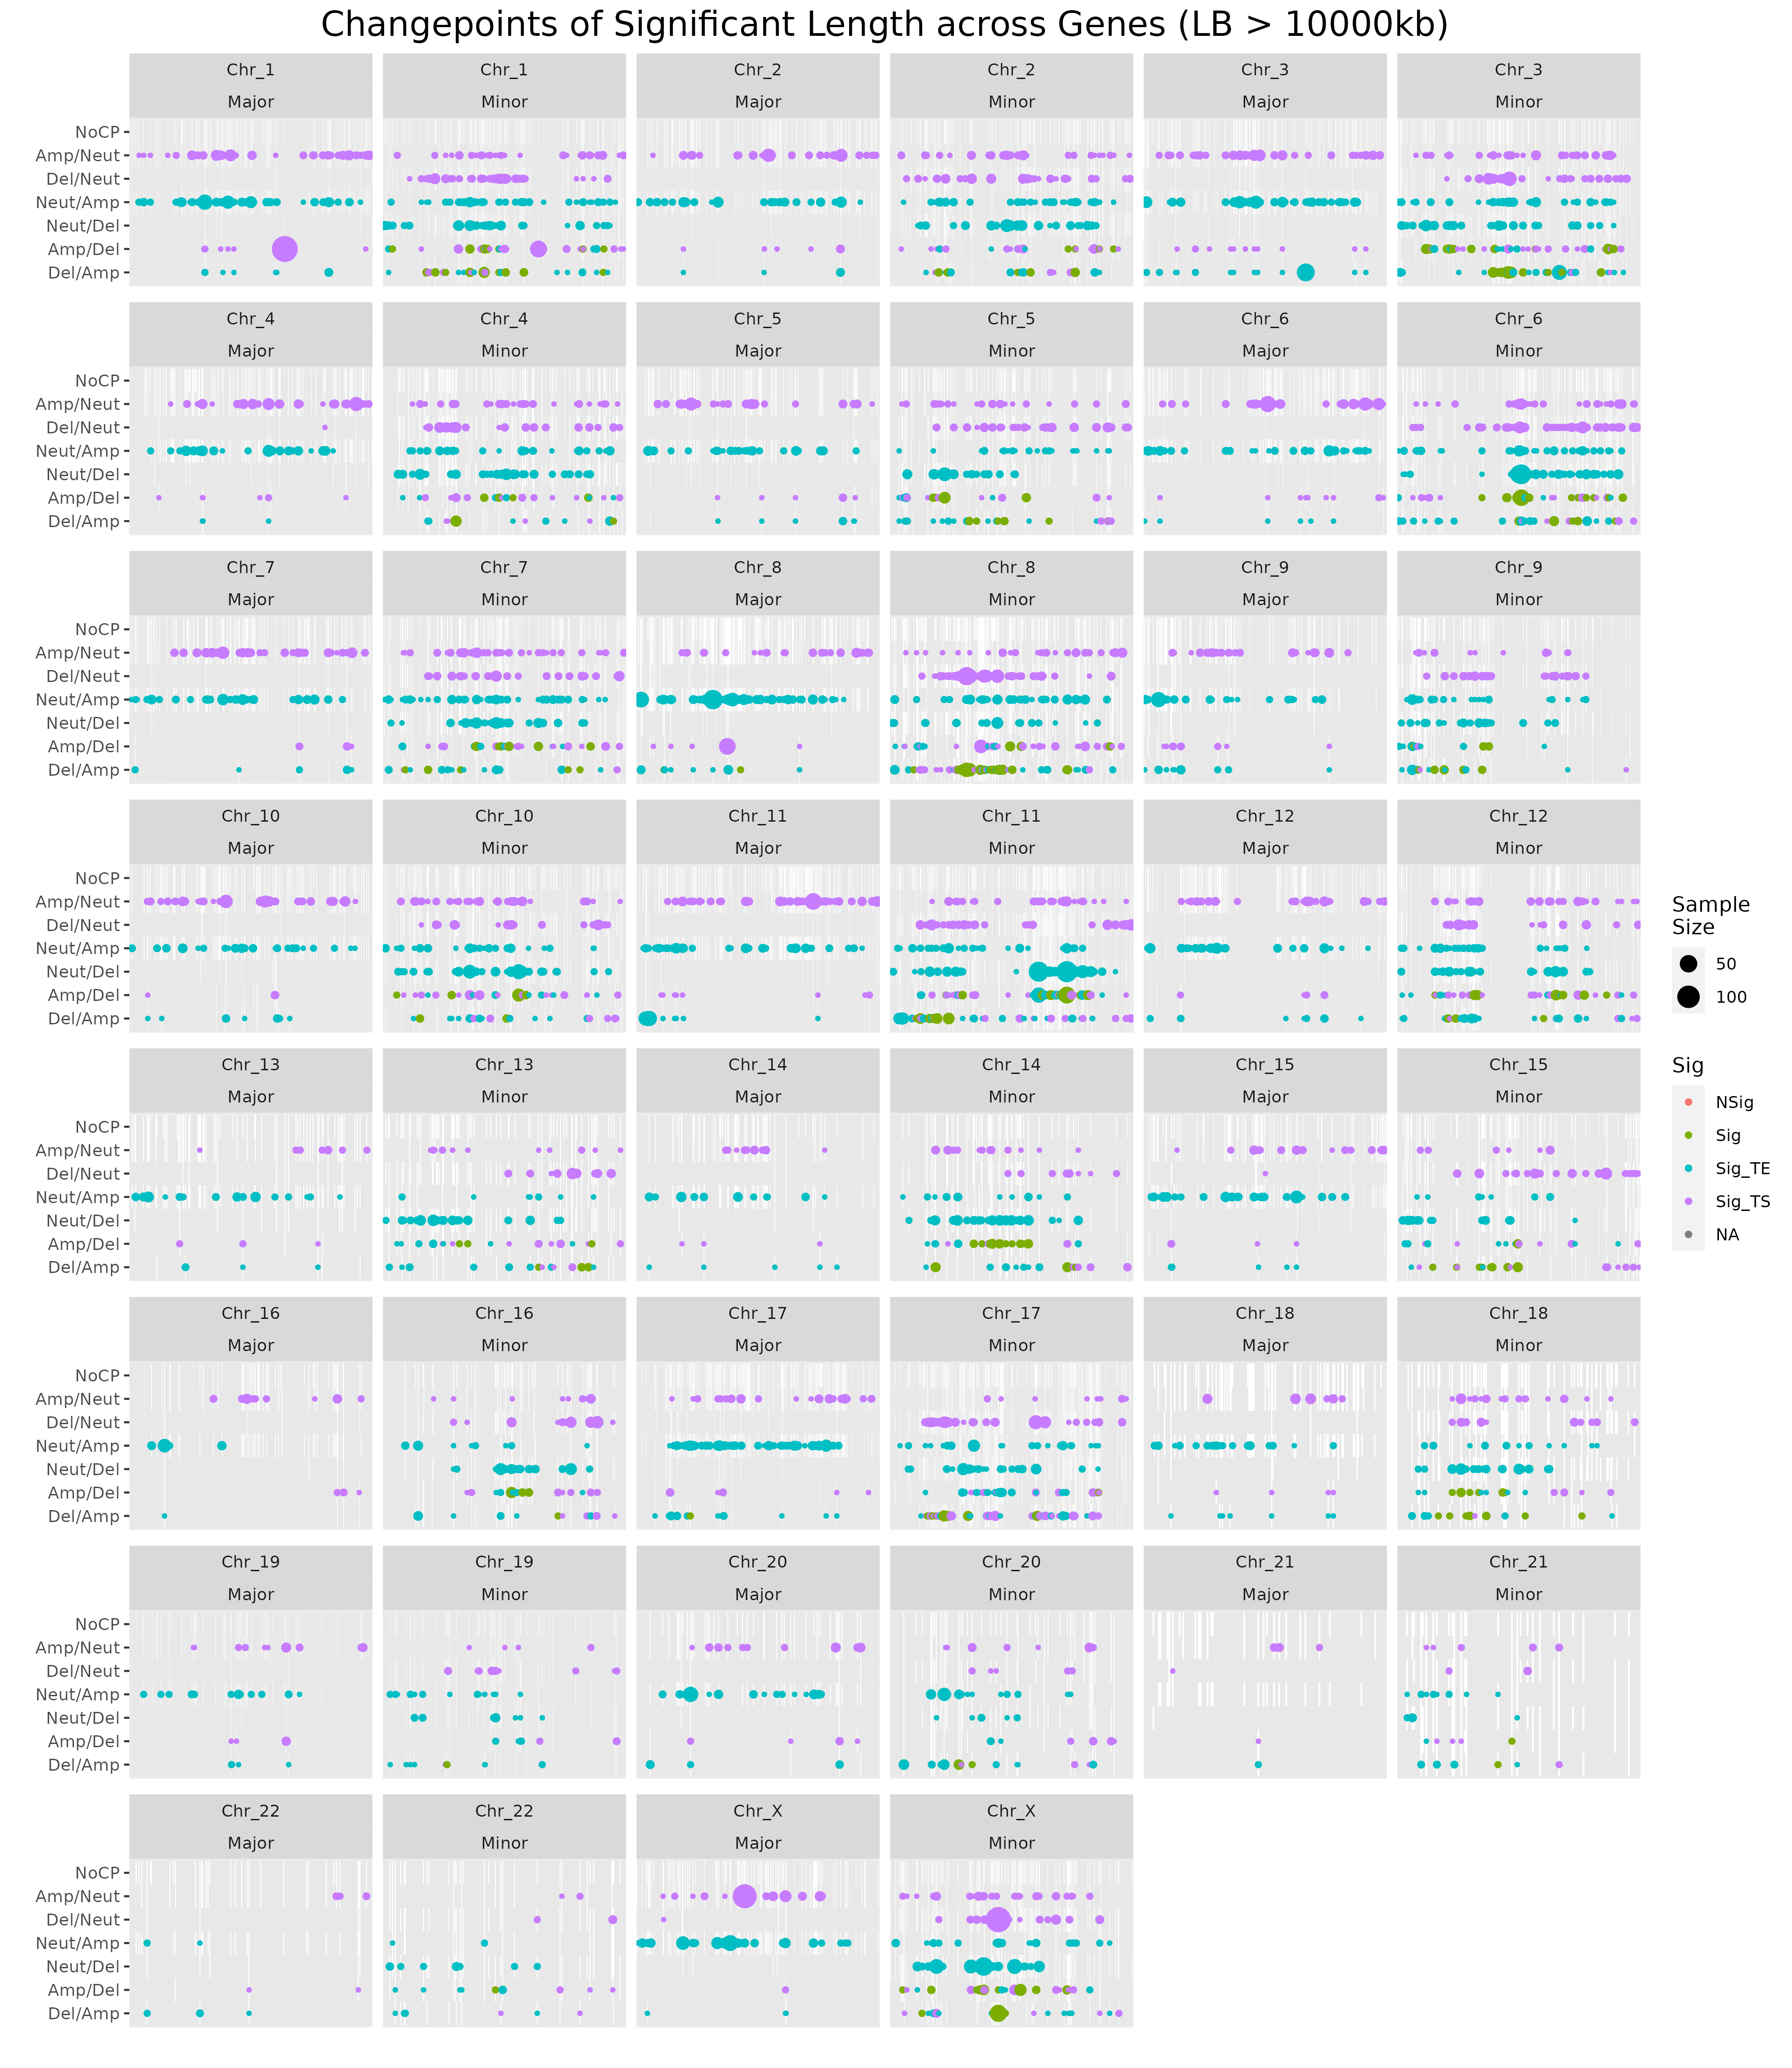
\includegraphics[width = 1\textwidth, height = 22cm]{../figures/Chapter_6/PerGene_MCMC_10000_Thesis.png}
\caption[Application of multivariate Allele-Dependent Intercept Model to each gene ($LB > 10,000$kb).]{Application of multivariate Allele-Dependent Intercept Model to each gene, providing confidence intervals for each category and allele. Each panel, corresponding to chromosome and allele, displays significance of changepoint determined by $LB > 10,000$kb. NoCP corresponds to NoChangepoint. Fitted using the \texttt{MCMCglmm()} function.}
\label{fig:PerGene_10000_MCMC}
\end{figure}

\begin{figure}[H]
\centering
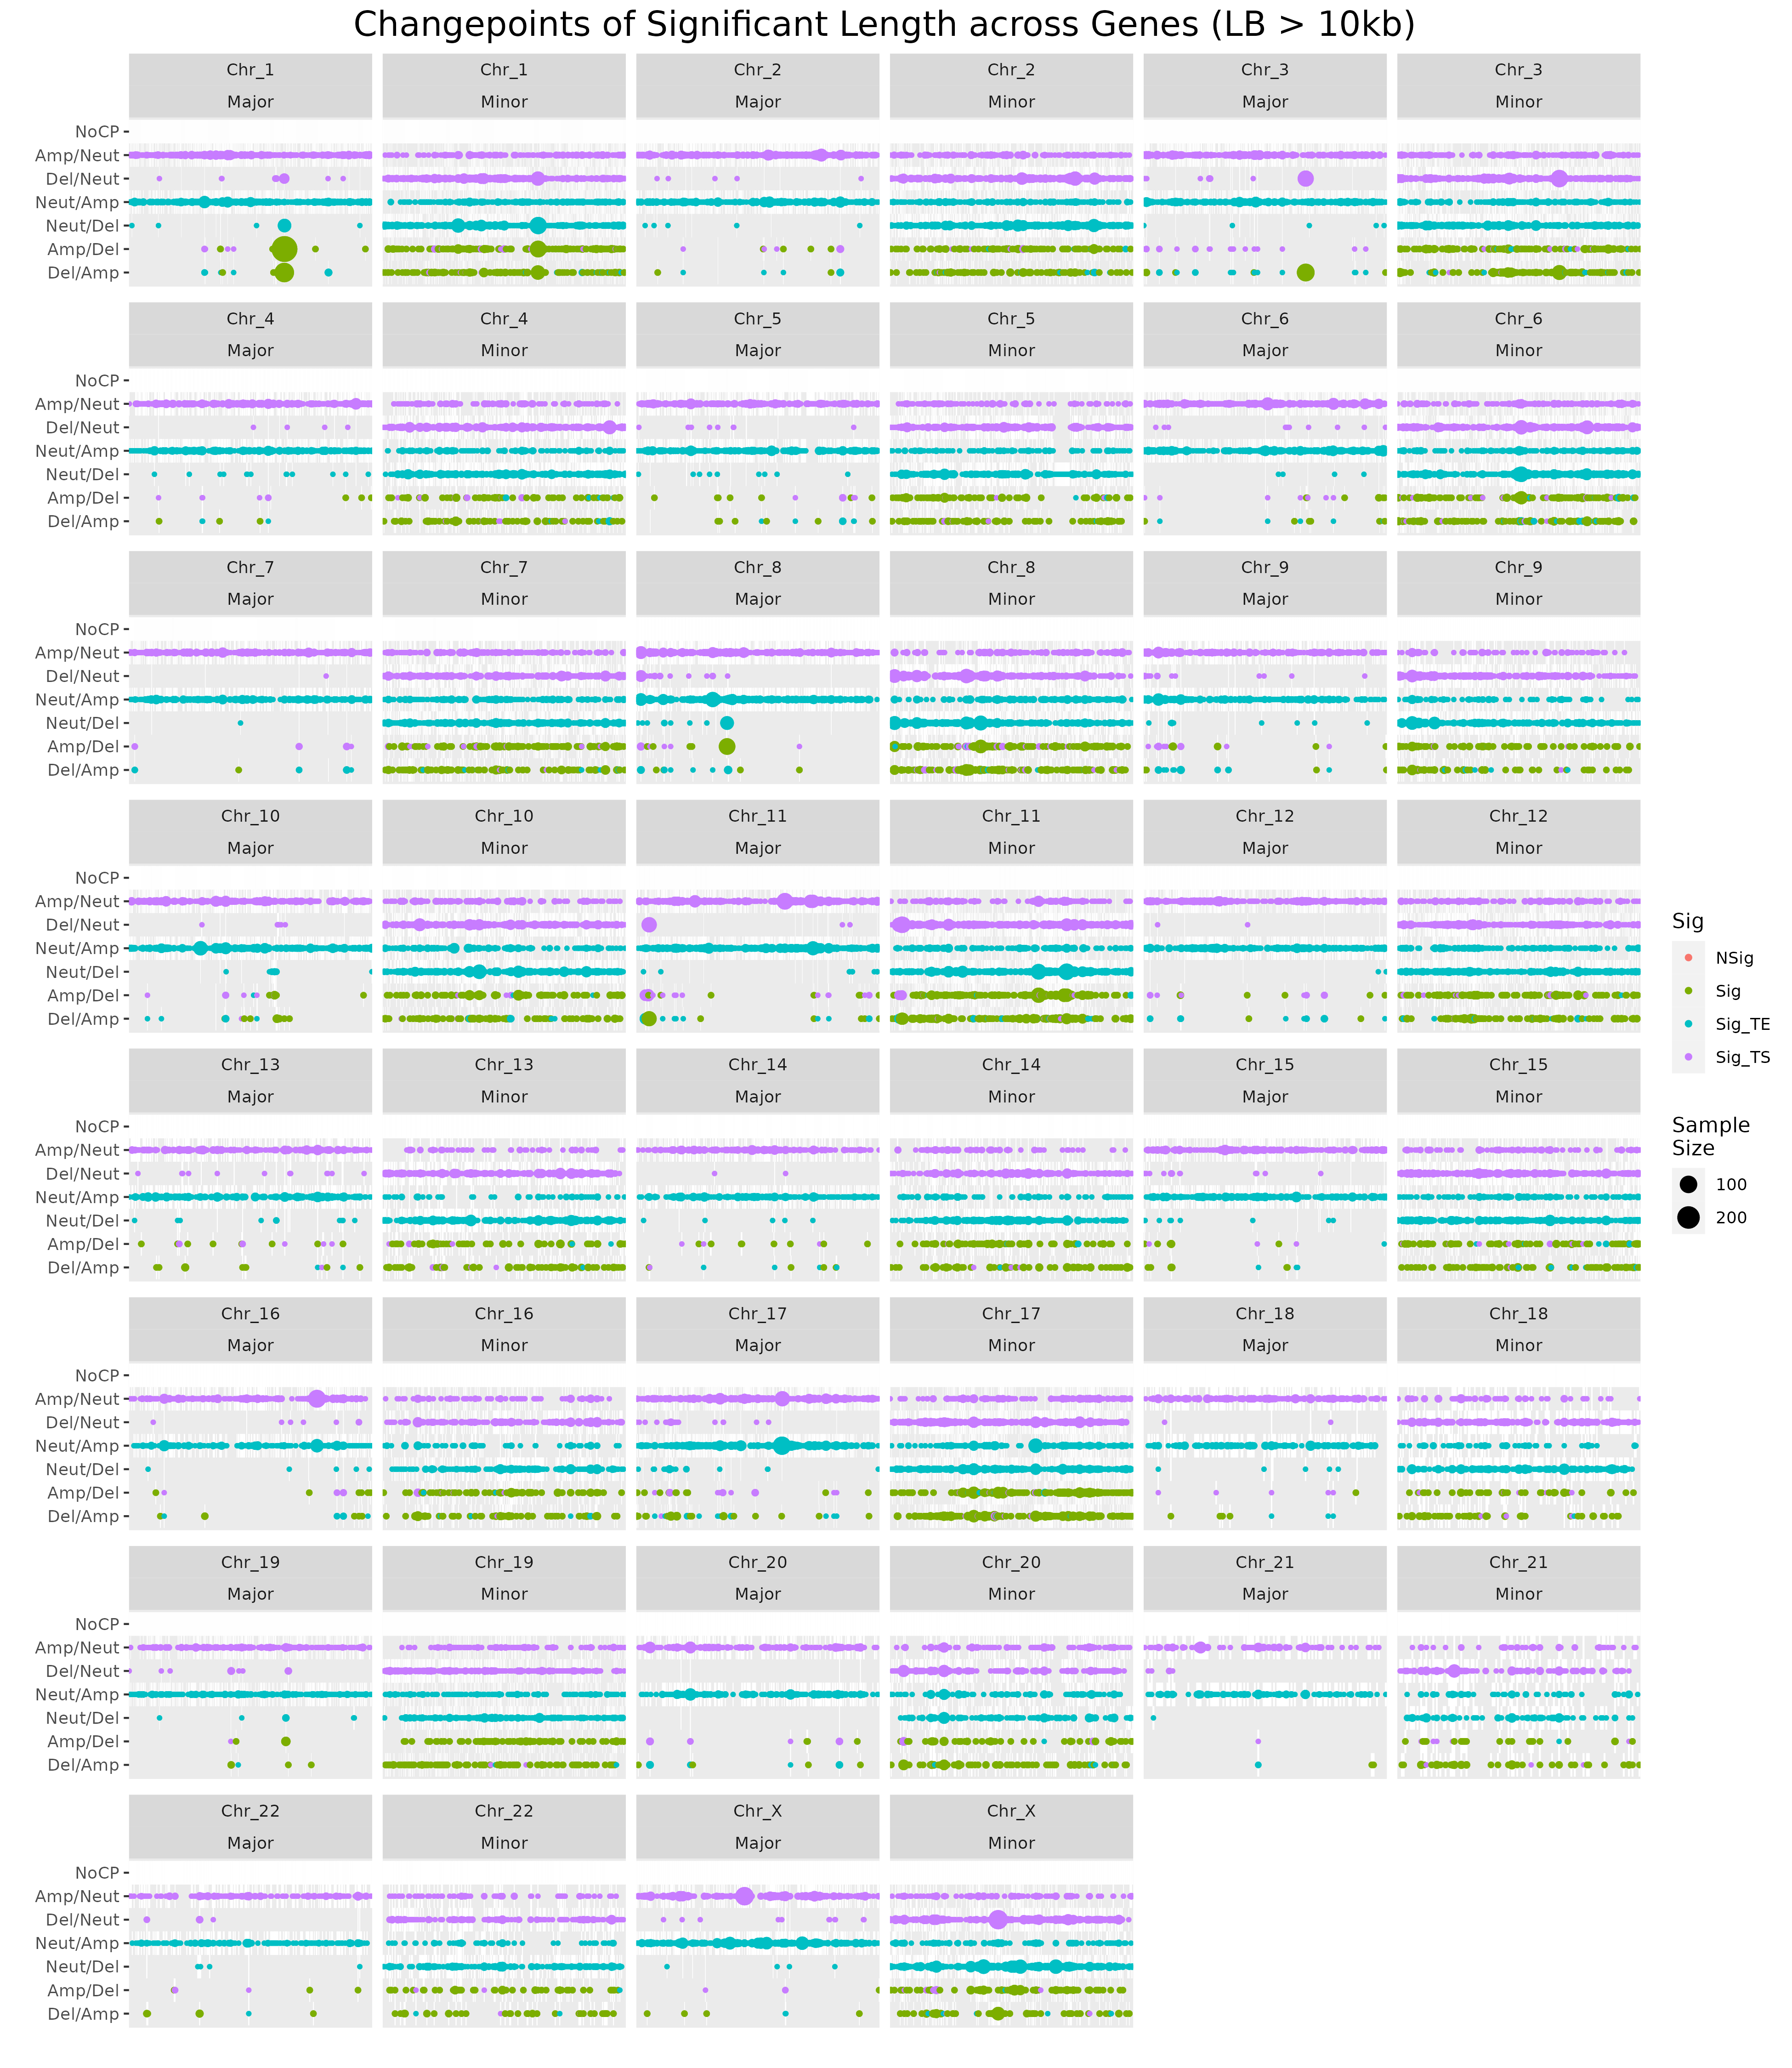
\includegraphics[width = 1\textwidth, height = 22cm]{../figures/Chapter_6/PerGene_LM_Zero_Thesis.png}
\caption[Application of univariate Allele-Dependent Intercept Model to each gene ($LB > 10$kb).]{Application of univariate Allele-Dependent Intercept Model to each gene, providing confidence intervals for each category and allele. Each panel, corresponding to chromosome and allele, displays significance of changepoint determined by $LB > 10$kb. NoCP corresponds to NoChangepoint. Fitted using the \texttt{lm()} function.}
\label{fig:PerGene_LM}
\end{figure}

\begin{figure}[H]
\centering
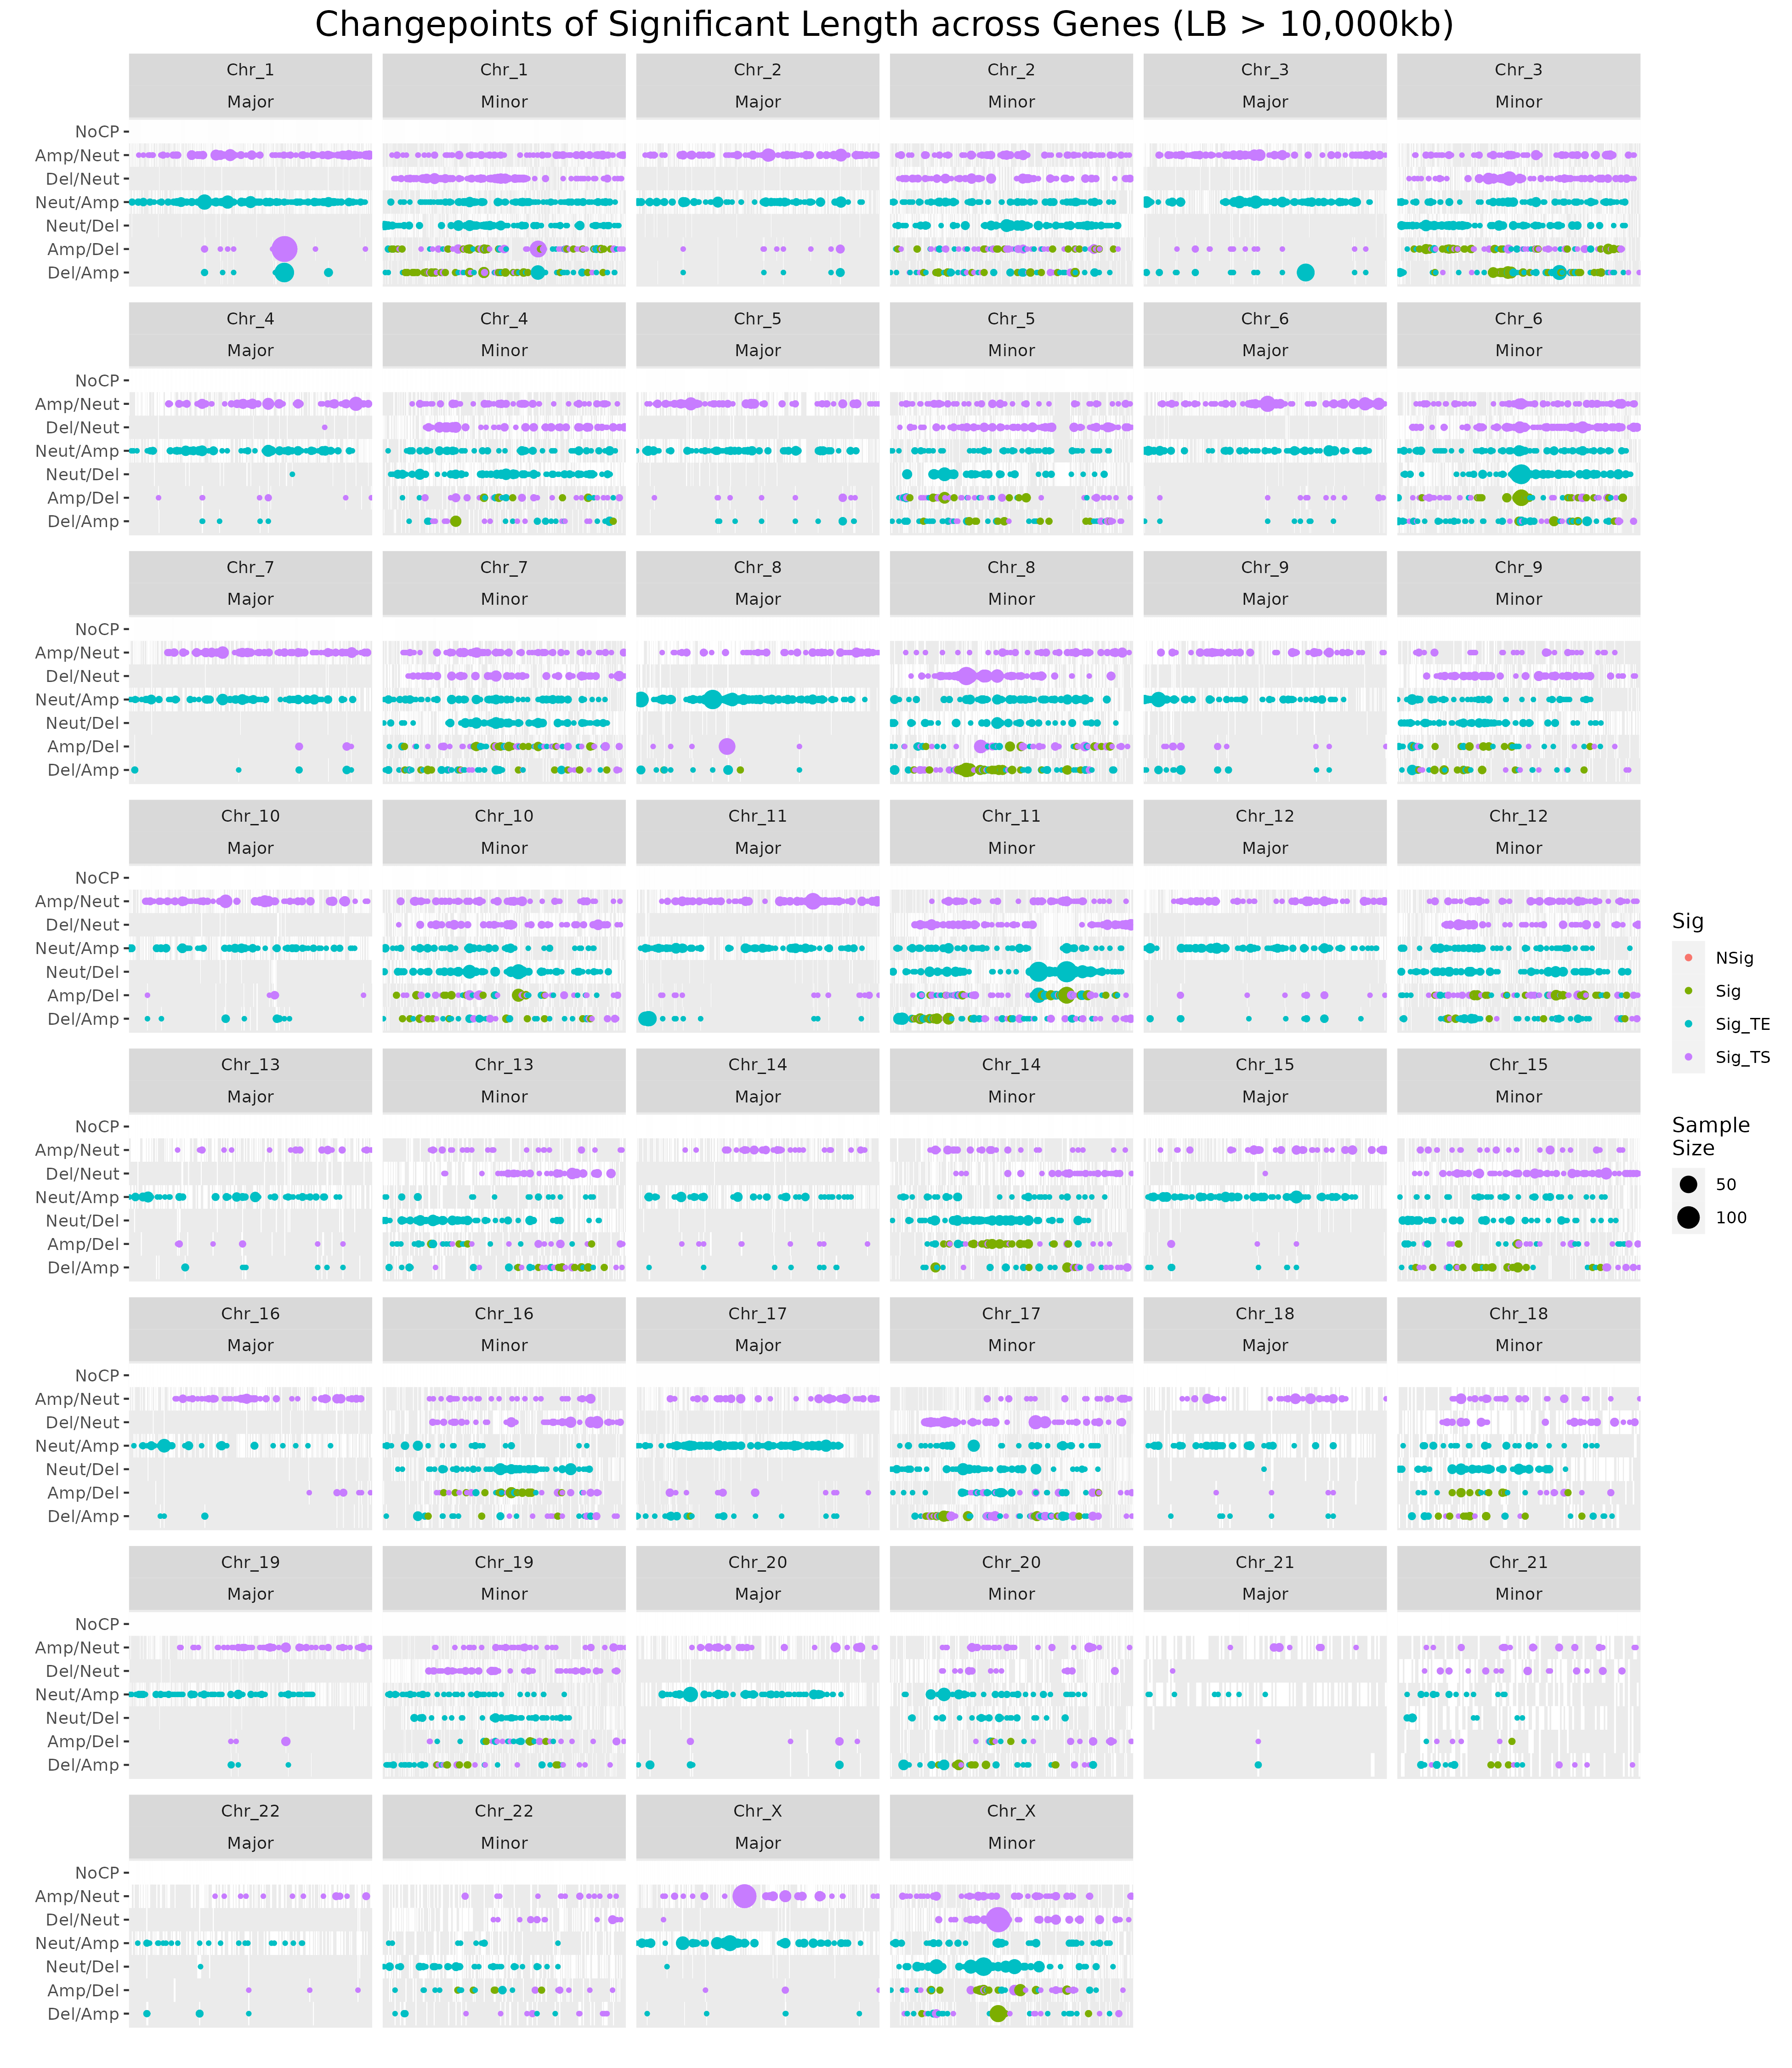
\includegraphics[width = 1\textwidth, height = 22cm]{../figures/Chapter_6/PerGene_LM_10000_Thesis.png}
\caption[Application of univariate Allele-Dependent Intercept Model to each gene ($LB > 10,000$kb).]{Application of univariate Allele-Dependent Intercept Model to each gene, providing confidence intervals for each category and allele. Each panel, corresponding to chromosome and allele, displays significance of changepoint determined by $LB > 10,000$kb. NoCP corresponds to NoChangepoint. Fitted using the \texttt{lm()} function.}
\label{fig:PerGene_10000_LM}
\end{figure}

\vfill
\begin{table}[!h]
\vspace{5cm}
\caption[Top 20 genes containing largest changepoints of significant length with $n > 30$ and $LB > 10,000$kb.]{Top 20 genes containing largest changepoints of significant length with $n > 30$ and $LB > 10,000$kb. Models fitted using (A) \texttt{MCMCglmm()} and (B) \texttt{lm()} functions.}
\centering
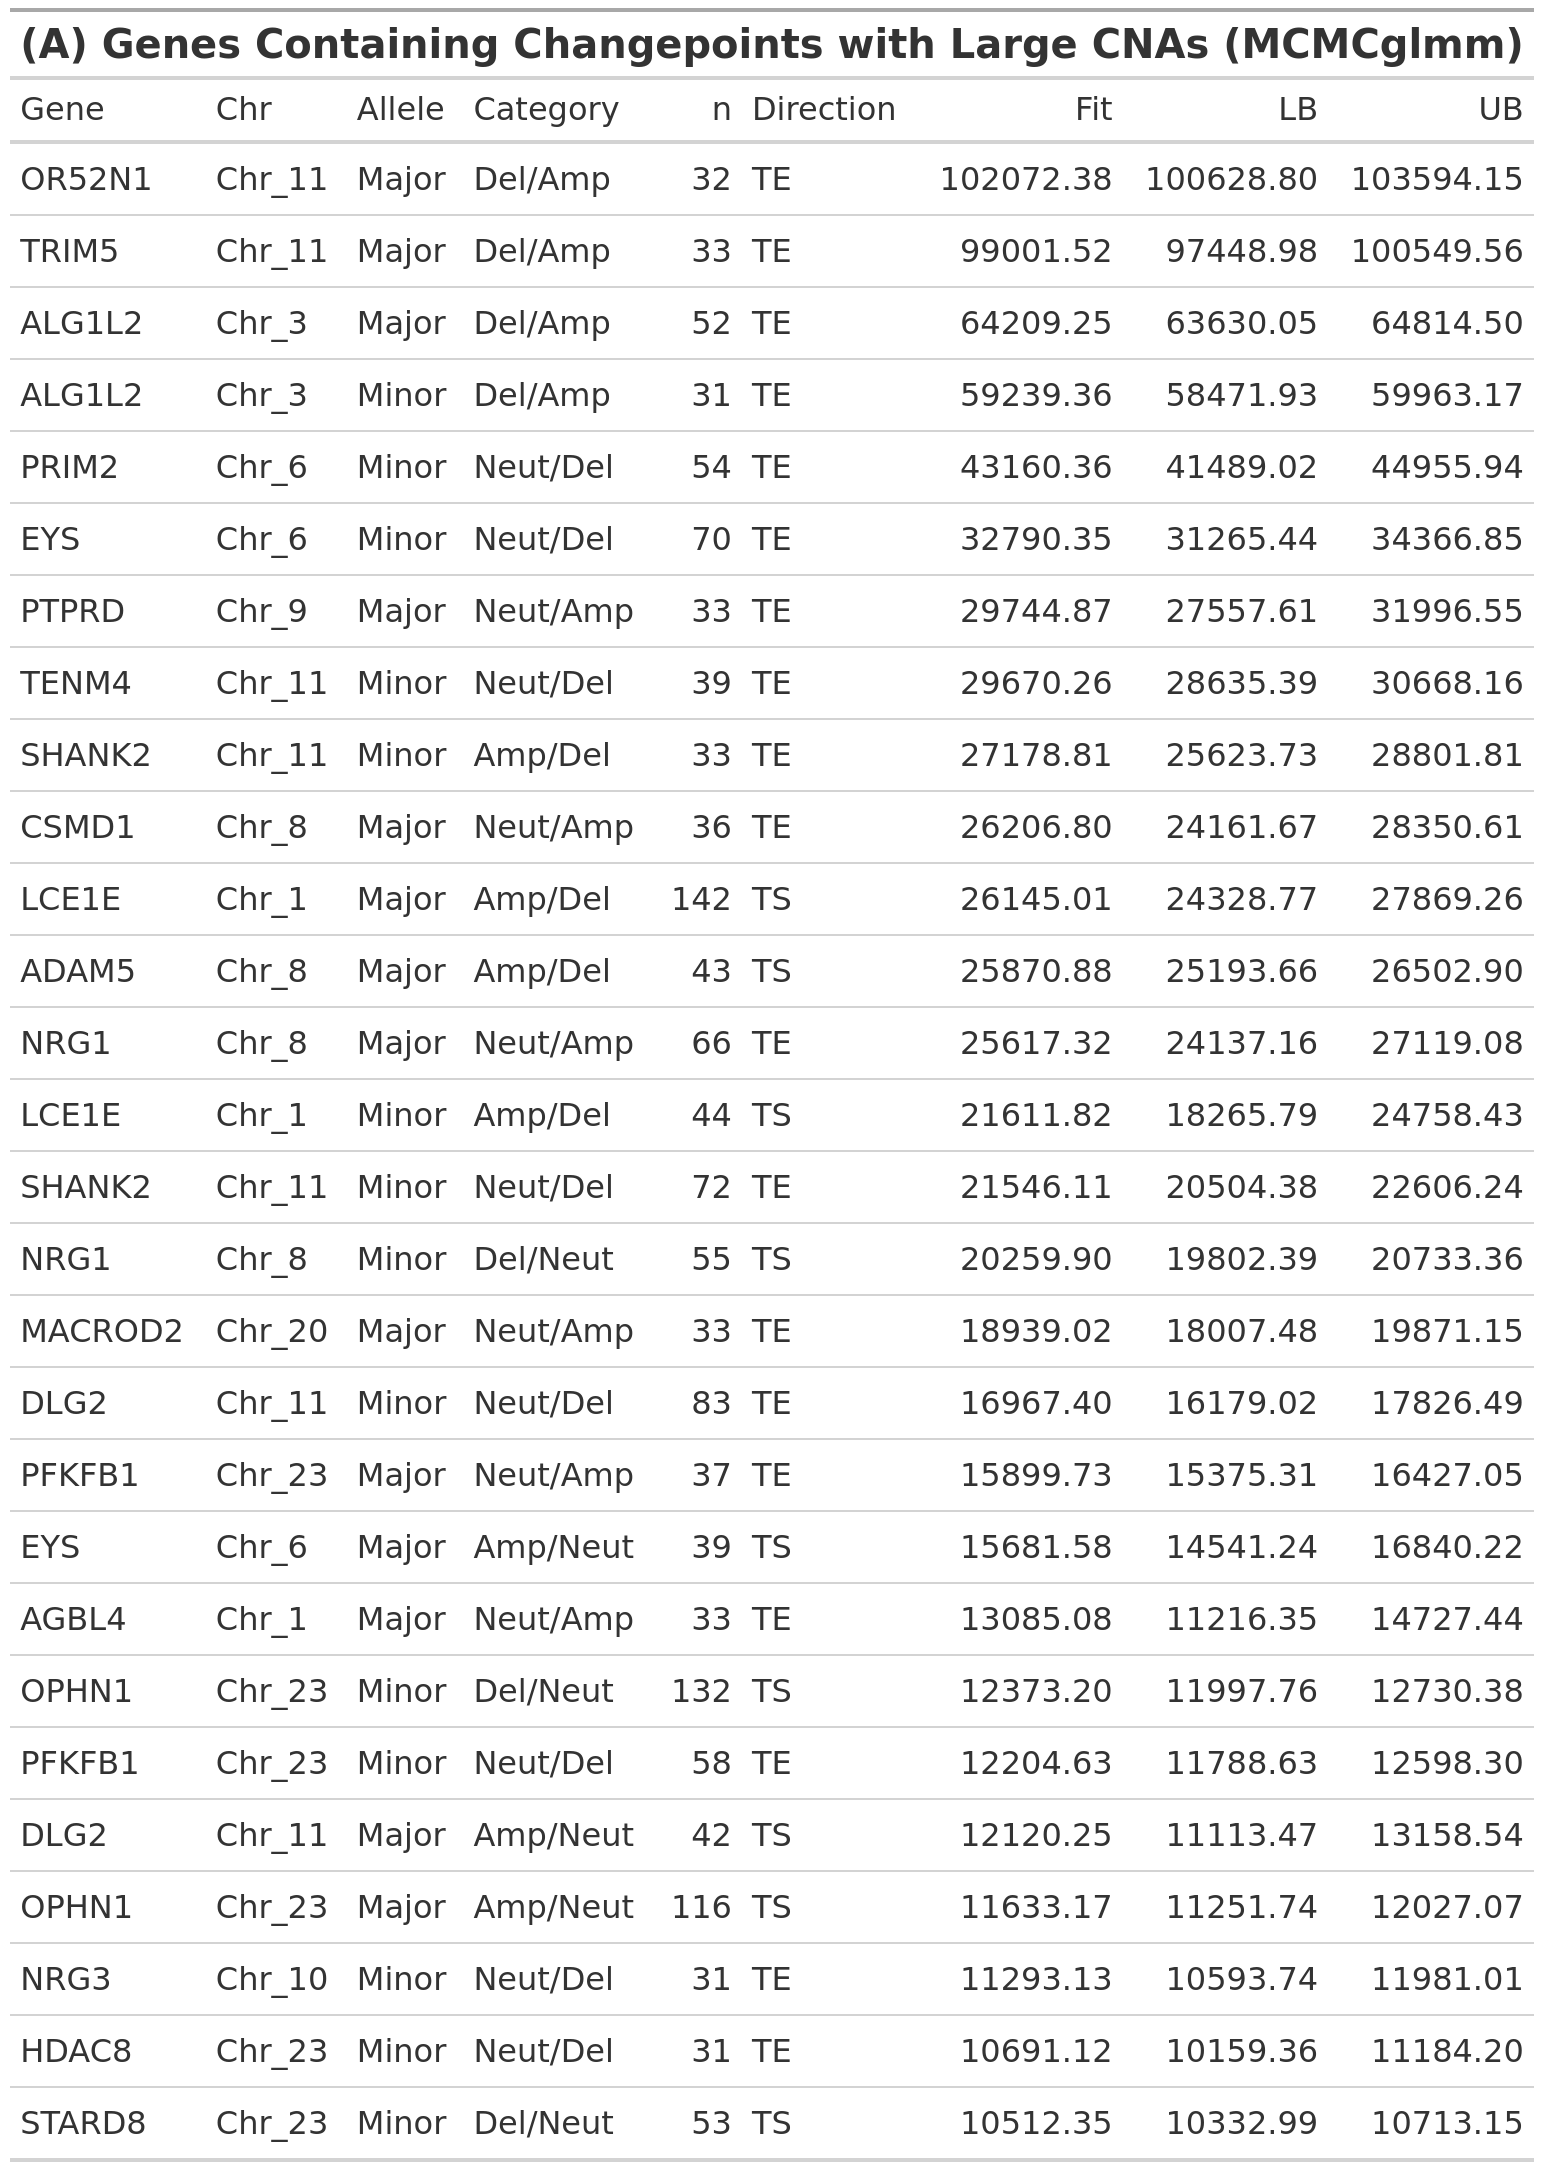
\includegraphics[width = 0.48\textwidth]{../tables/Chapter_6/Gene_MCMC_1_Thesis.png}
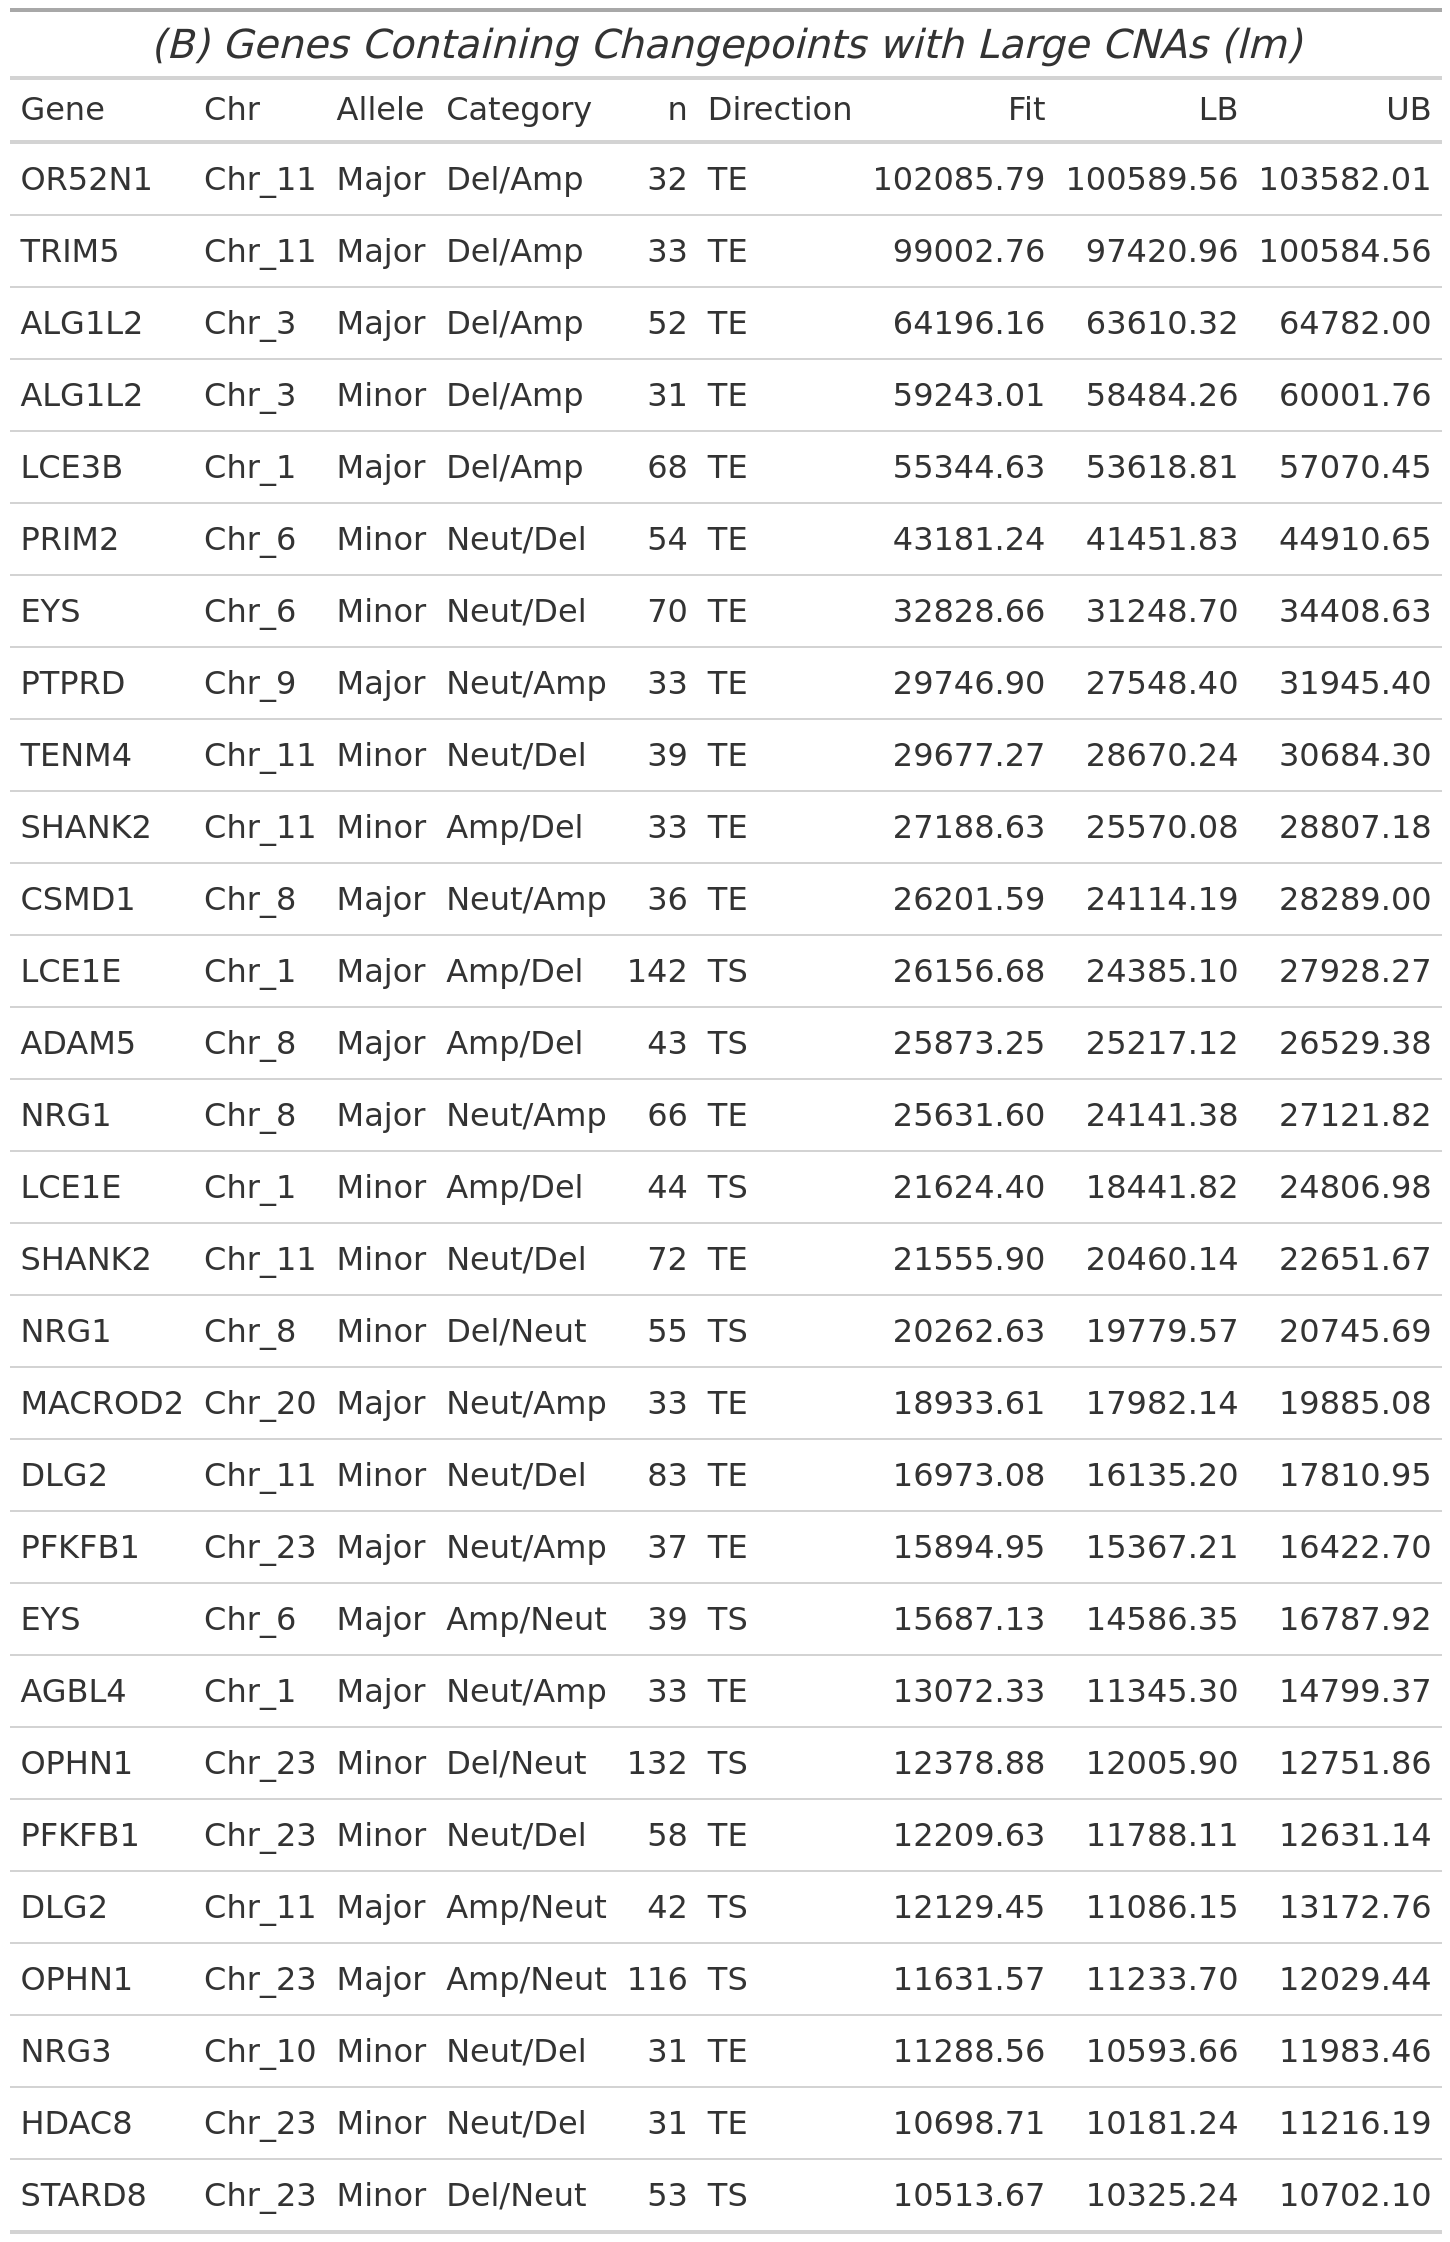
\includegraphics[width = 0.48\textwidth]{../tables/Chapter_6/Gene_LM_1_Thesis.png}
\label{tab:TopLength_Genes_1}
\end{table}
\vfill

\begin{figure}[H]
\centering
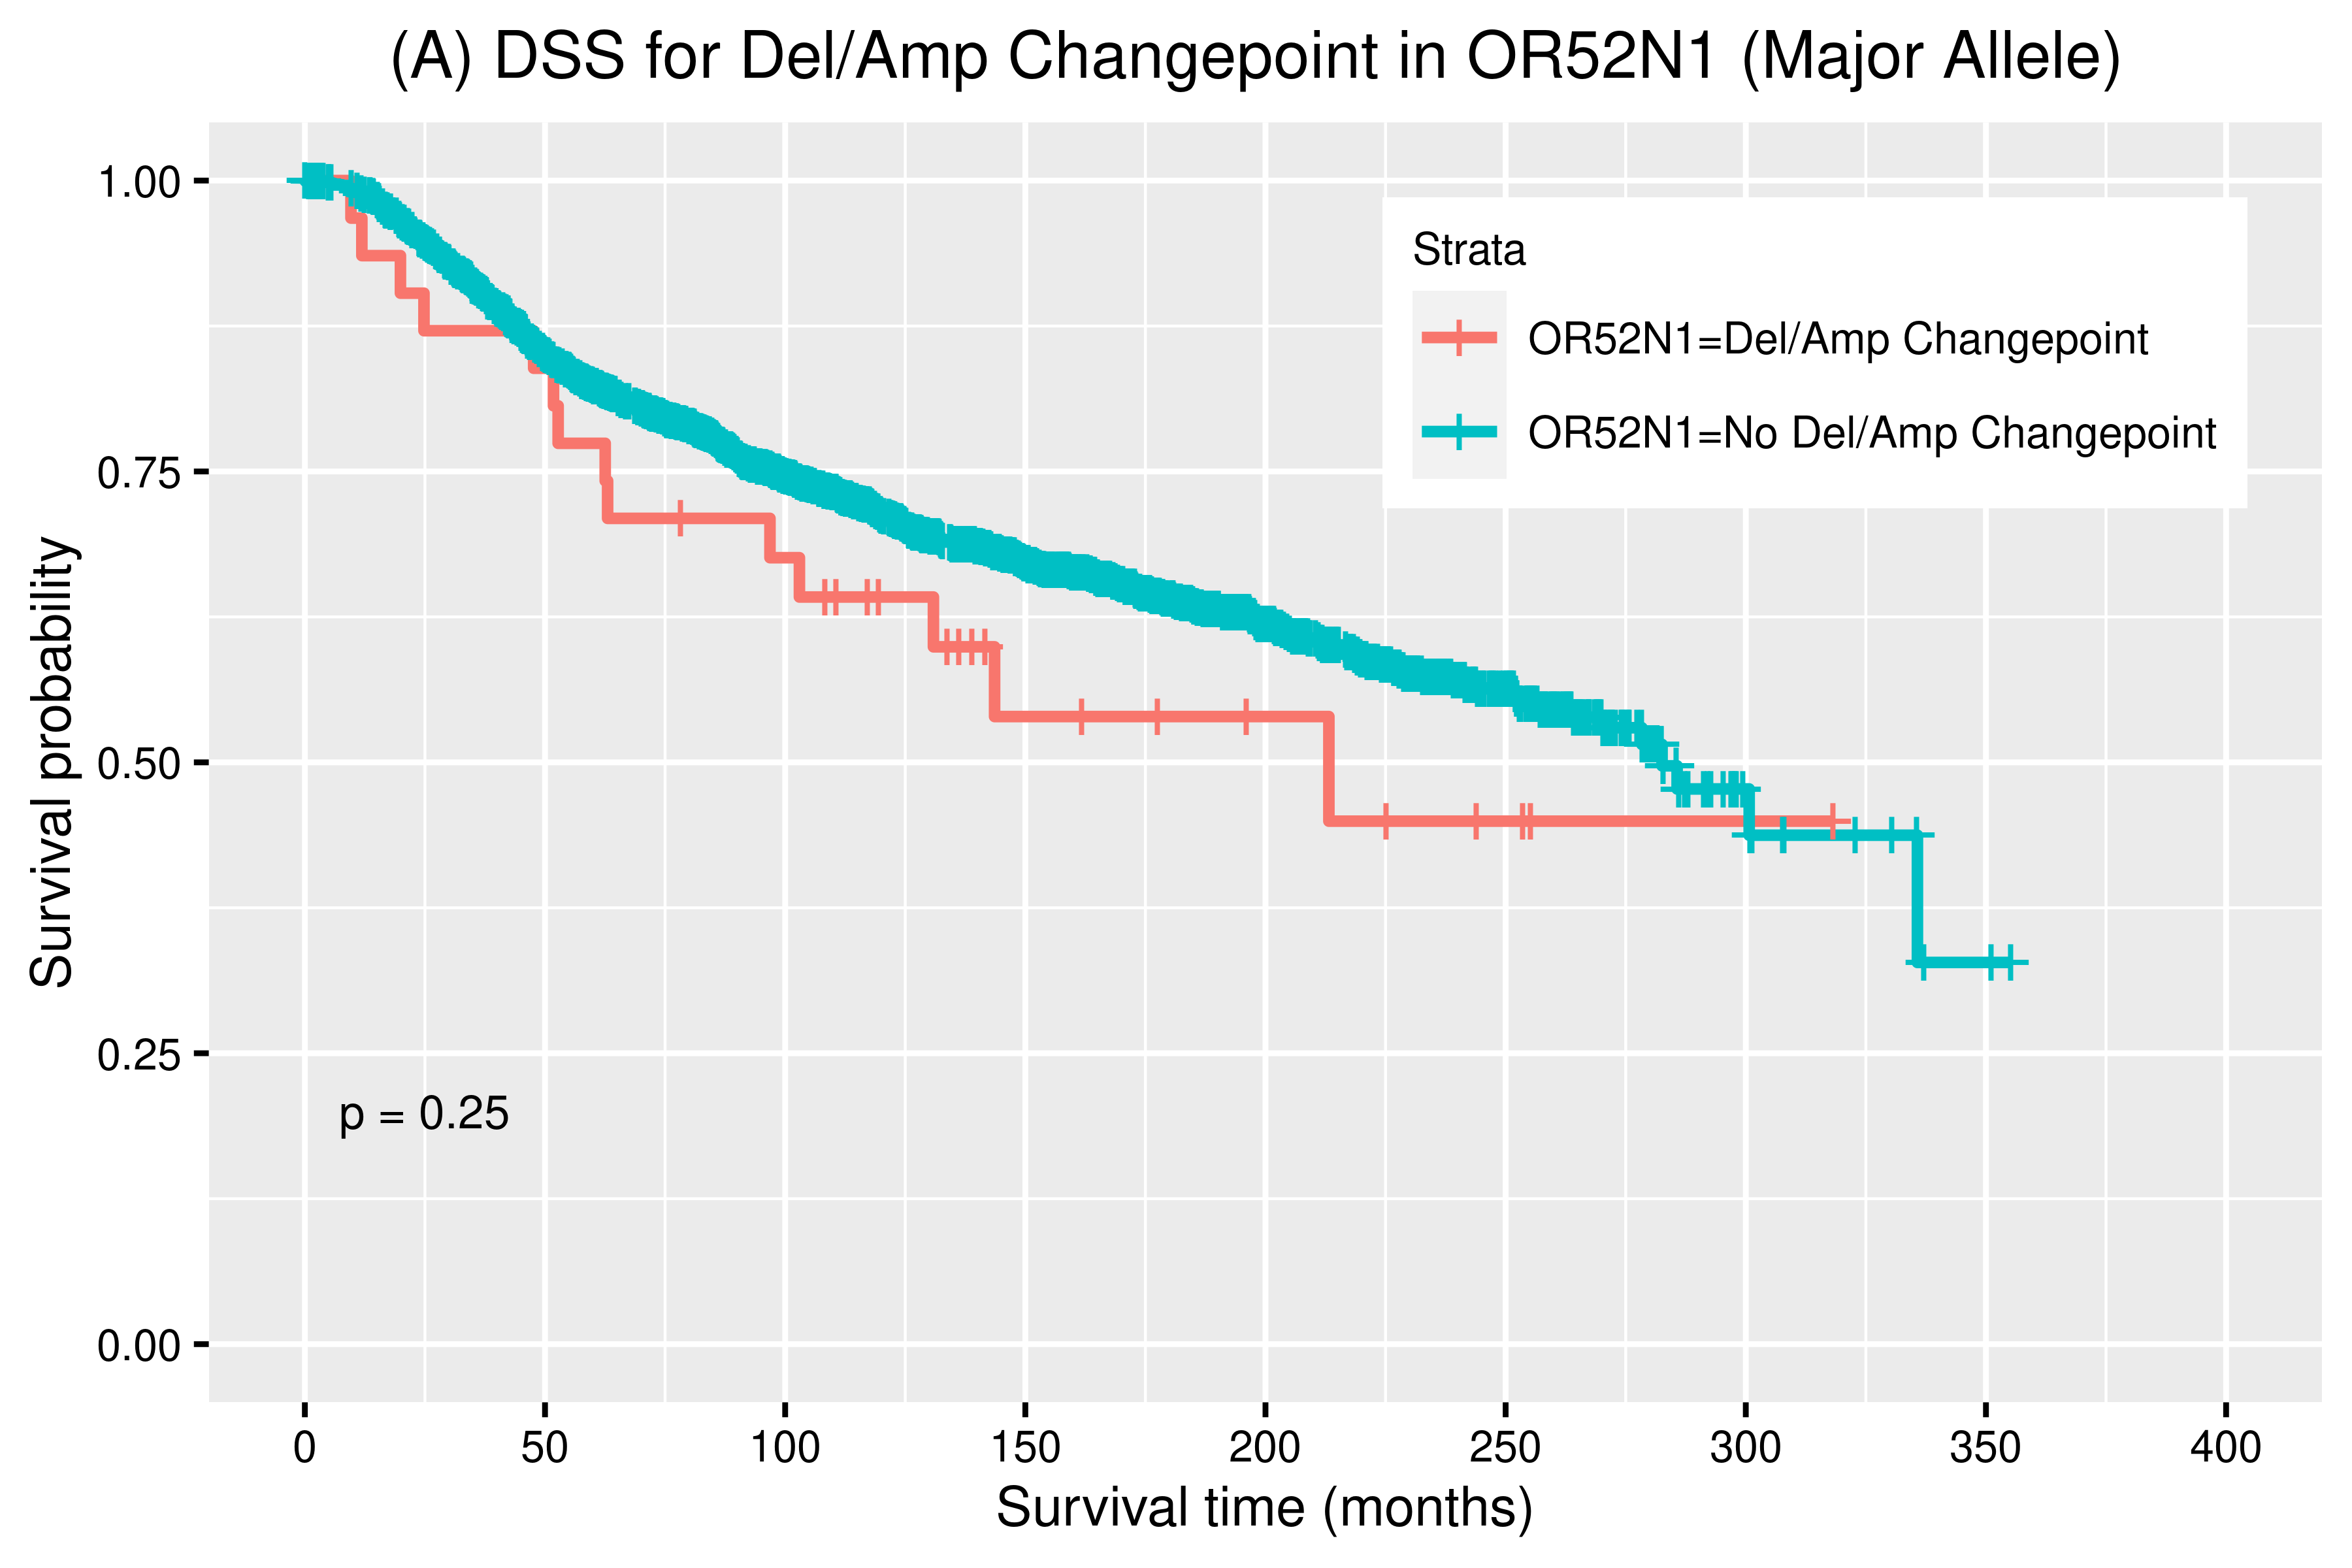
\includegraphics[width = 0.48\textwidth]{../figures/Chapter_6/survplot_OR52N1.png}
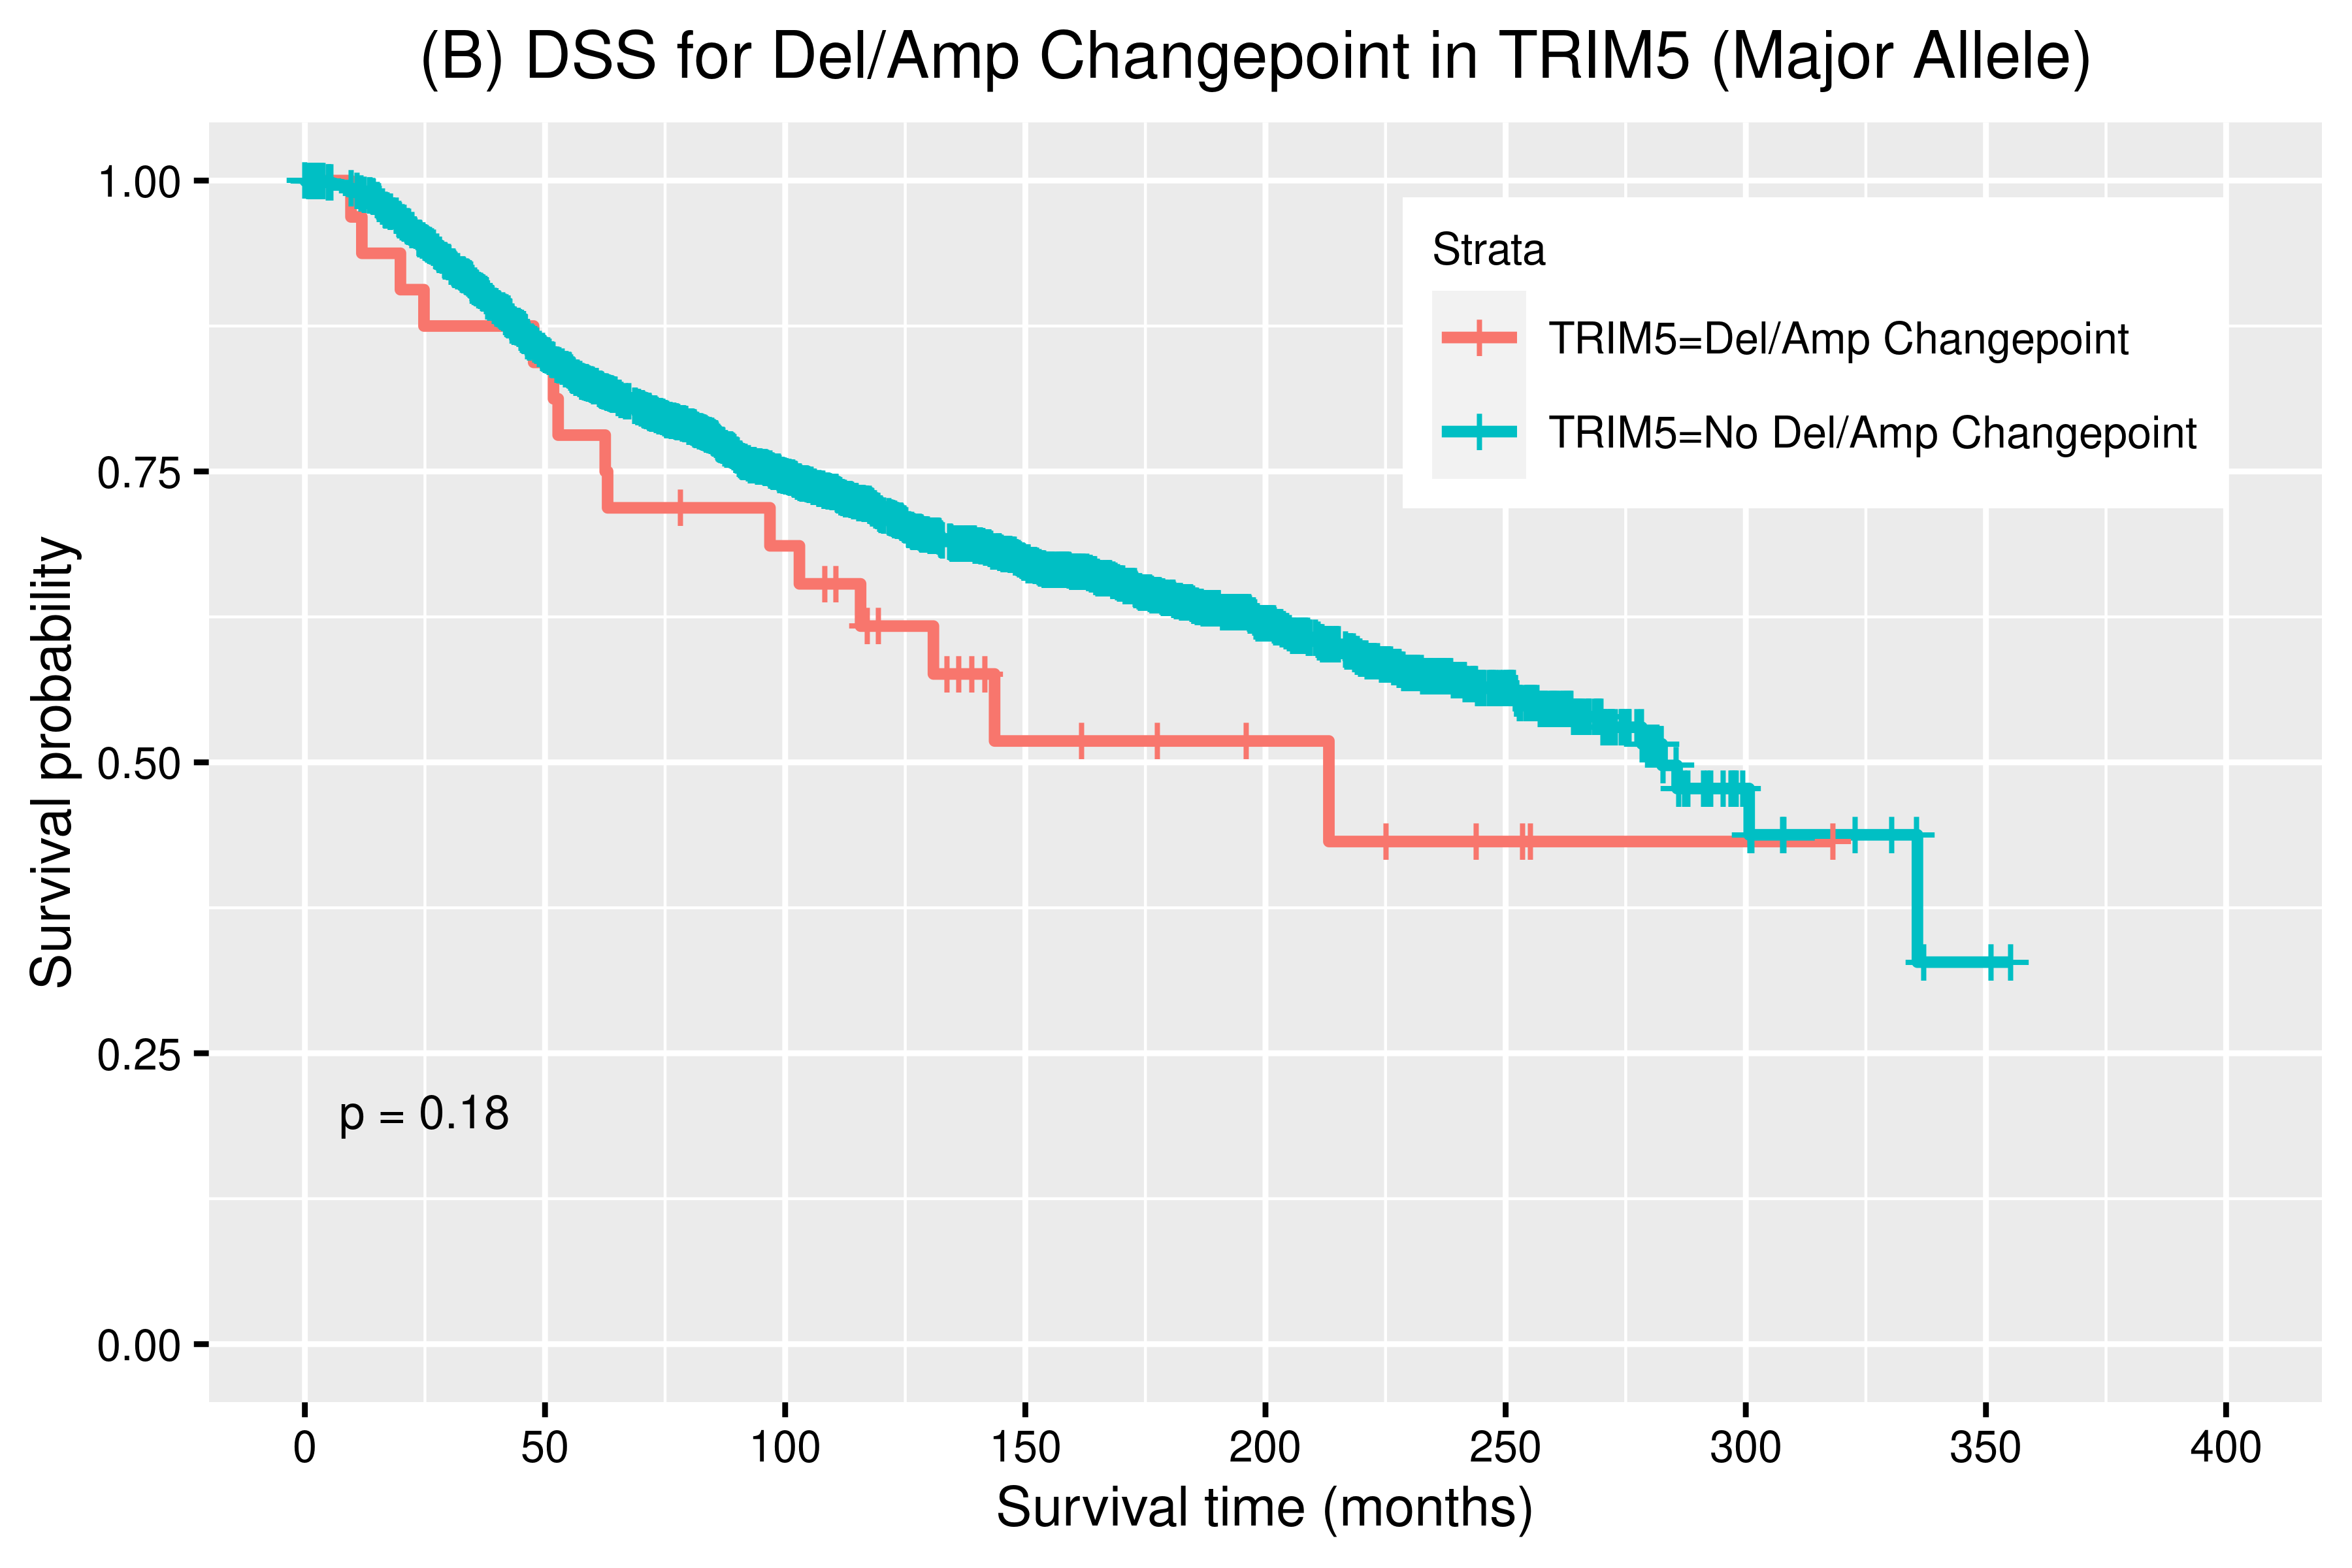
\includegraphics[width = 0.48\textwidth]{../figures/Chapter_6/survplot_TRIM5.png}
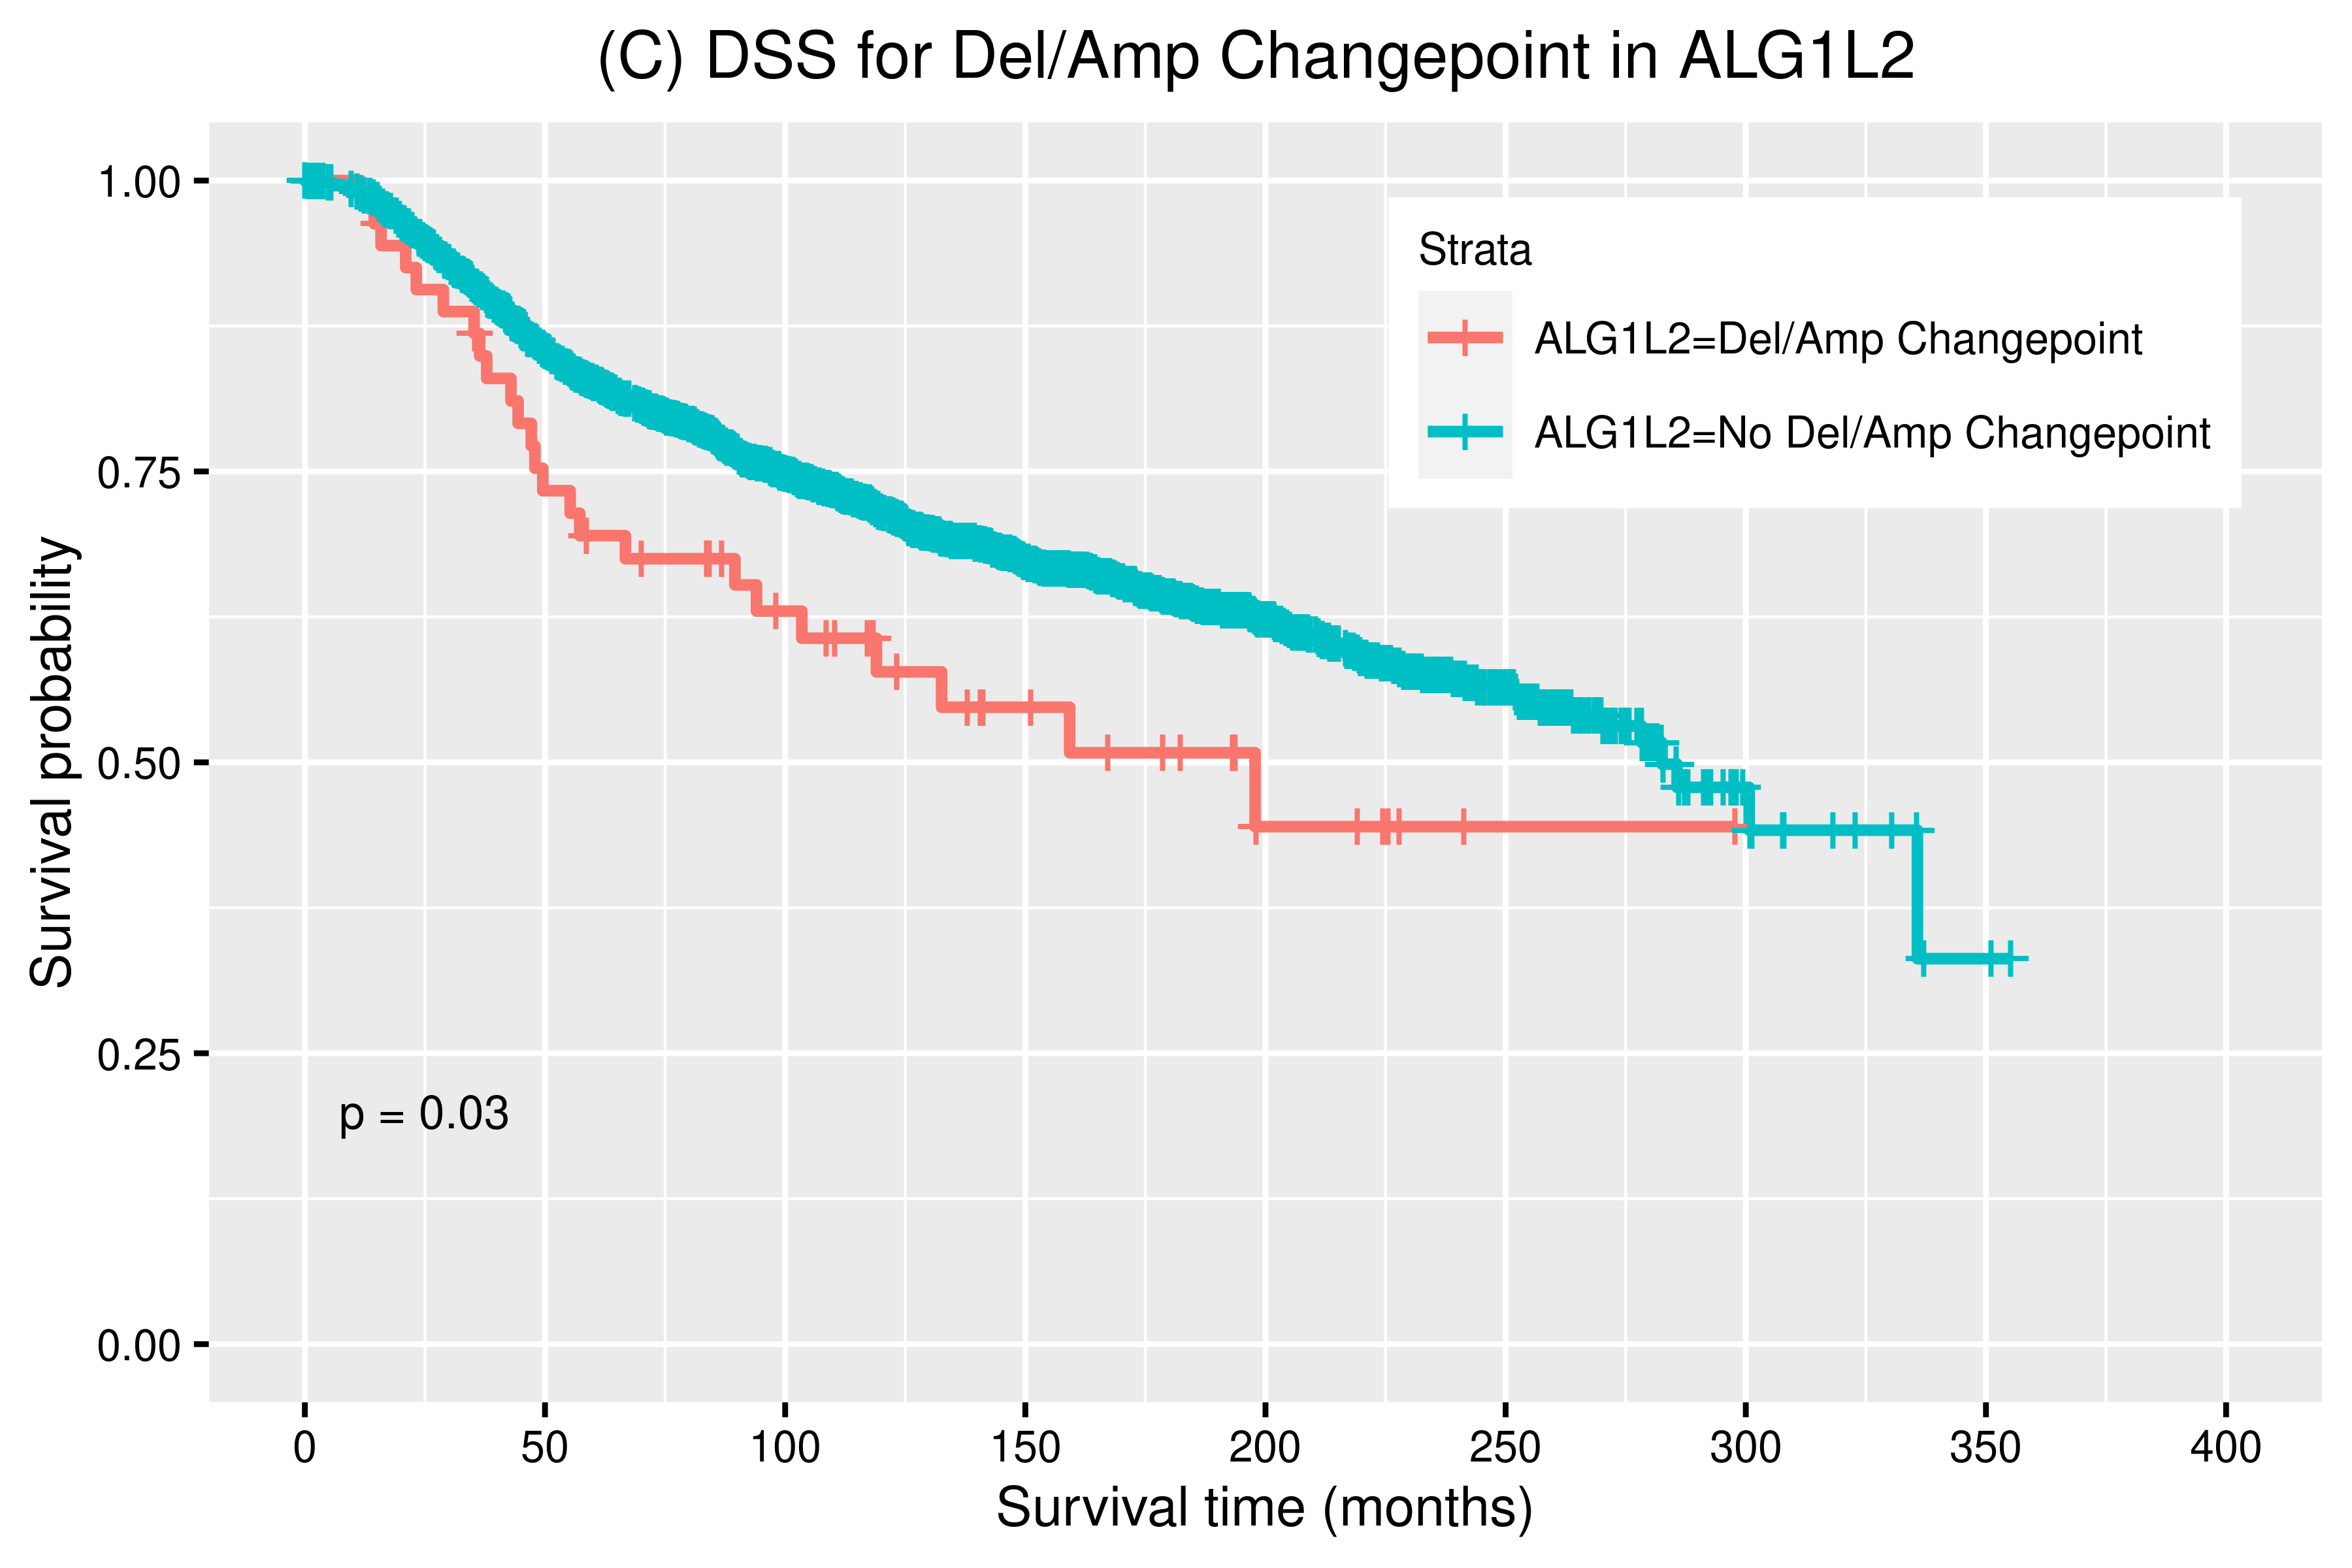
\includegraphics[width = 0.48\textwidth]{../figures/Chapter_6/survplot_ALG.png}
\caption[Survival curves for changepoints in selected genes.]{Survival curves for changepoints in selected genes. (A) OR52N1 (B) TRIM5 and (C) ALG1L2.}
\label{fig:TopLength_Genes_Surv}
\end{figure}

\subsection{Whole-genome Allele-specific Changepoints across Chromosomes}
Genomic regions attributed to genes, as analysed in the last section, make up only a small proportion of the total length of the human genome. The ASCAT data provides us with whole genome allele-specific copy number profiles, from which the gene regions were extracted previously. In this section, we carry out a broader analysis across the whole genome by segmenting the genome into consecutive equal distances of a pre-determined value $d$. Applying ADIM within each segmented region detects changepoints across the whole genome region with significant length of the changepoint states, $TS$ and/or $TE$. 

\subsubsection{Genome Segmentation}
Figure \ref{fig:Histogram_Total} displays the frequency and category of changepoints across the genome. To determine over what distance $d$ the AD model will be applied, consideration is given to number of options including a sliding window approach, a per chromosome/chromosome arm approach or a segmentation approach, where the genome is split into segments of constant length using varying distances, e.g. setting $d$= 5,000kb, 5 million bases. For the genome segmentation method, segmentation is applied across each chromosome, starting at the first observed genomic location and ending at the last observed genomic location. Each segment will be the same length across the chromosome except for the last segment which will be of varying length. 

\begin{figure}[H]
\centering
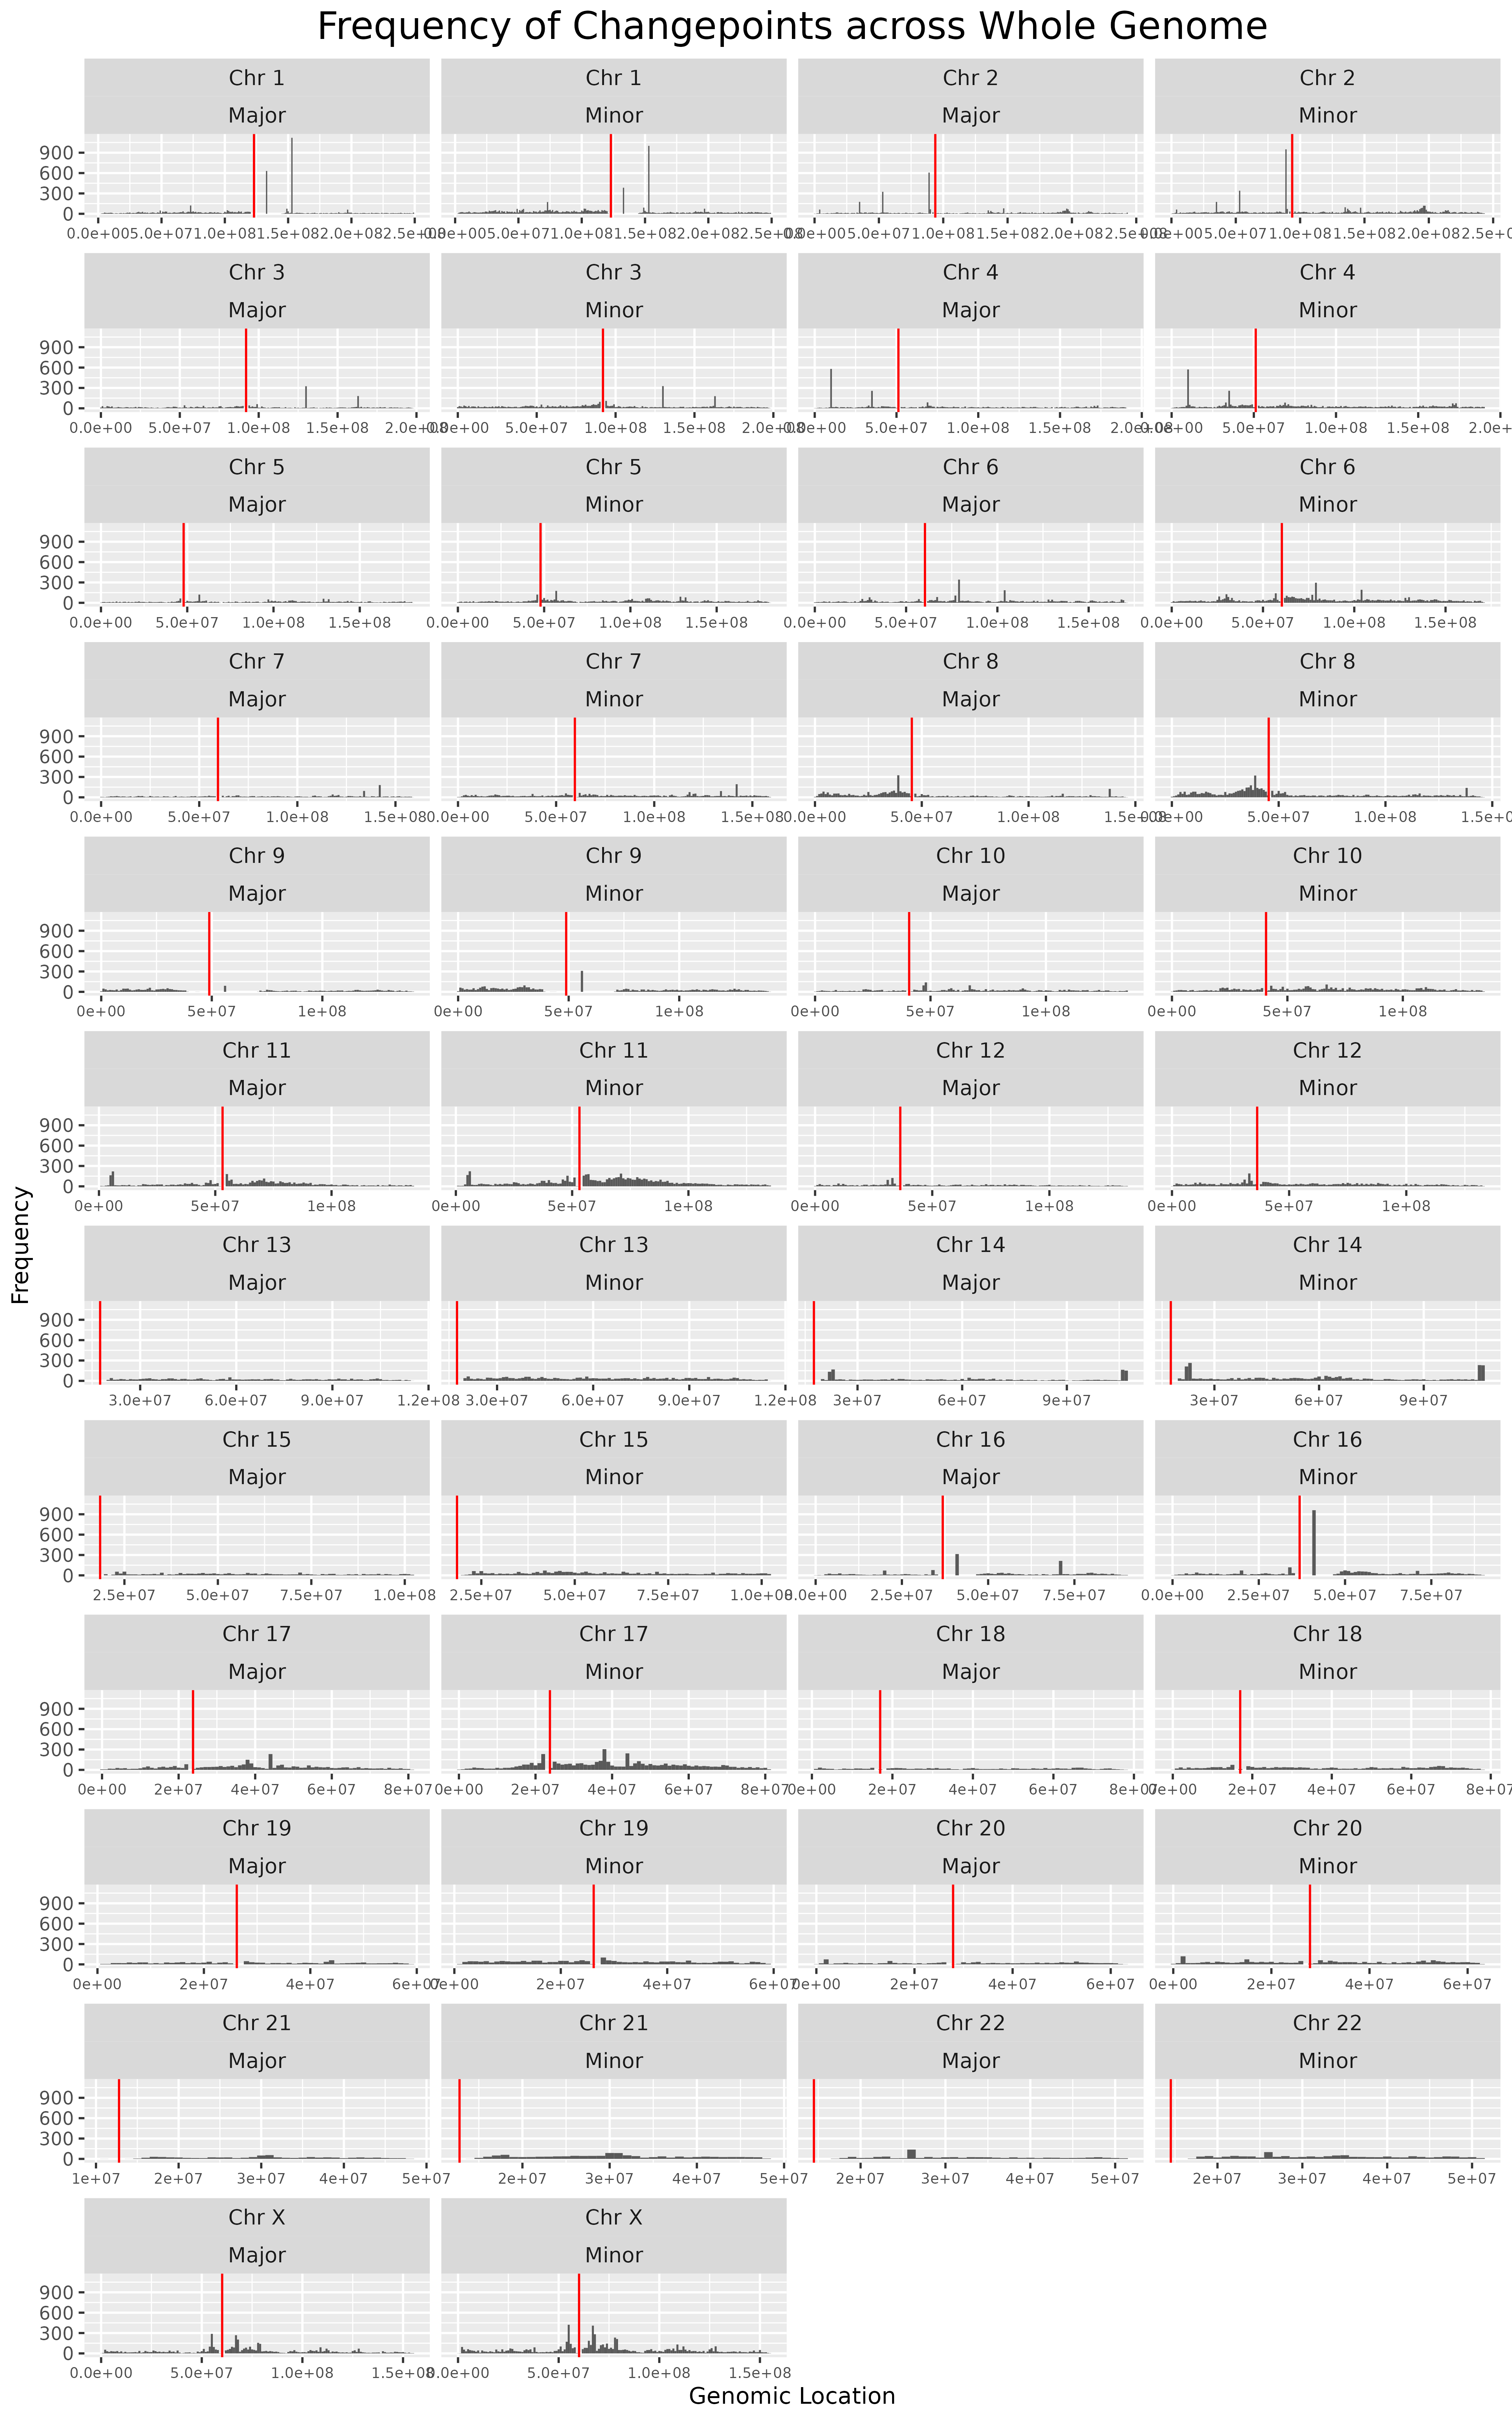
\includegraphics[width = 1\textwidth, height = 23cm]{../figures/Chapter_6/Scaled_Frequency_Genomic_Seg.png}
\caption[Frequency of changepoints across the whole genome for each chromosome and allele.]{Frequency of changepoints across the whole genome for each chromosome and allele. Scale of y-axis is the same across all chromosomes and the red line indicates the midpoint of the centromere.}
\label{fig:Histogram_Total}
\end{figure}

\subsubsection{Outcomes of Selected Models to Segmented Regions}
Out of 603 segmented regions of $d$=5,000kb, nine do not display any changepoint and are omitted from the analysis. For the remaining 594 genomic segments, the AD model is successfully applied to 591 genomic segments using the \texttt{MCMCglmm()} function. The three failed segments are segment 29 on chromosome 1, segment 28 on chromosome 10 and segment 8 on chromosome 16, and these likely require a stronger or proper prior to be implemented. The tile plot highlighting segments across the genome containing changepoints with $TS$ or $TE$ greater than 10kb indicates that most segments contain at least one changepoint with average length greater than 10kb (Figure \ref{fig:PerSegment_MCMC}). While the presence of changepoints is widespread, chromosomes containing changepoints with a large number of observations and $TS$ and/or $TE$ lengths significantly greater than 10kb include chromosome 1, 2, 8, 11, 16, 17 and X (Figure \ref{fig:PerSegment_MCMC}). 

\begin{figure}[!hp]
\centering
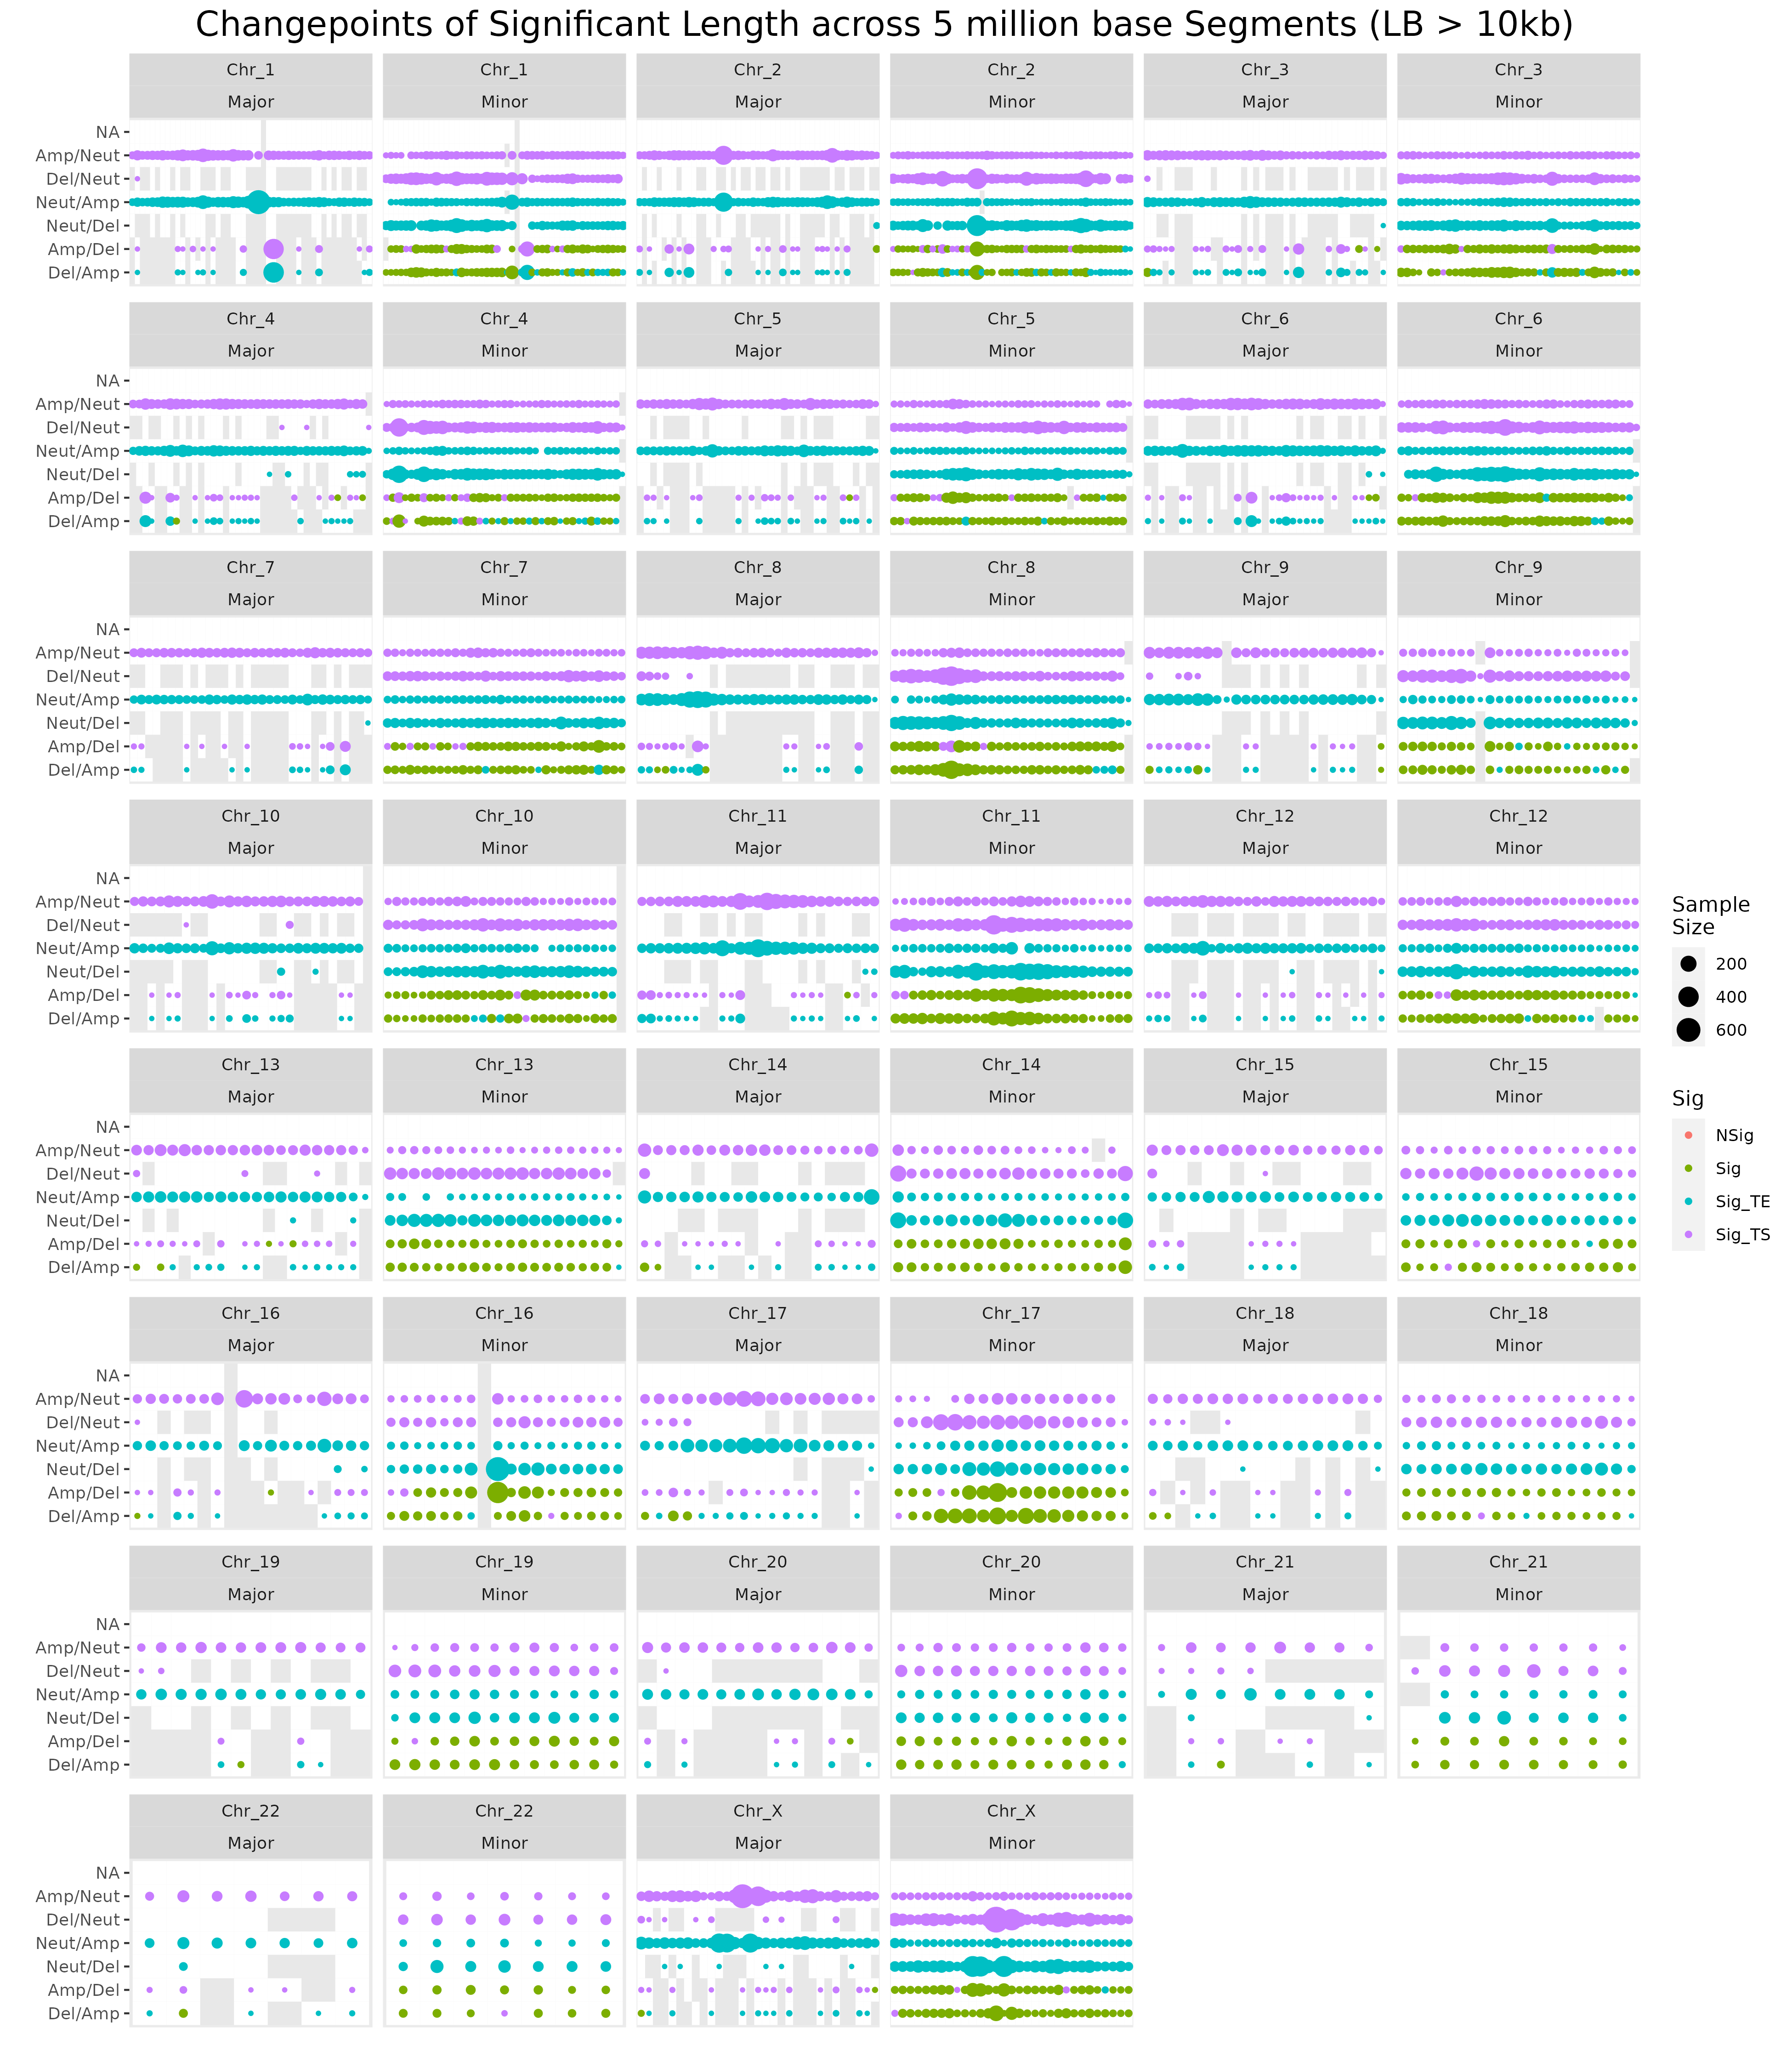
\includegraphics[width = 1\textwidth, height = 22cm]{../figures/Chapter_6/PerSegments_MCMC_10kb_fivemillion_Thesis.png}
\caption[Application of multivariate Allele Dependent Intercept Model to each segment, providing prediction intervals for each category and allele. Significance determined by $LB > 10$kb.]{Application of multivariate Allele Dependent Intercept Model to each segment, providing prediction intervals for each category and allele. Each panel, corresponding to chromosome and allele, displays significance of changepoint, determined by $LB > 10$kb. NoCP corresponds to NoChangepoint. Fitted using the \texttt{MCMCglmm()} function.}
\label{fig:PerSegment_MCMC}
\end{figure}
%\FloatBarrier
Similarly,  the tile plot showing segments across the genome containing changepoints with $TS$ and/or $TE$ lengths greater than 10,000kb indicates that despite the increased average length threshold from 10kb to 10,000kb, a large number of segments still contain at least one changepoint of average length greater than 10,000kb in at least one patient (Figure \ref{fig:PerSegment_MCMC_10000}). Chromosomes containing notable changepoints - those with a large number of observations and average length significantly greater than 10,000kb - include chromosome 1, 8, 11, 16 and X (Figure \ref{fig:PerSegment_MCMC_10000}).

Fitting the multivariate ADIM MCMCglmm indicates 591 unique segments across the genome contain at least one changepoint with an average length significantly greater than 10kb, with 588 having an average length over 10,000kb. Focusing on the AD models imposing sample size filtering, $n > 100$ and $n > 200$, results in 97 and 22 unique segments across the genome containing changepoints with an average length significantly greater than 10kb and 38 and 11 unique segments across the genome containing changepoints with an average length significantly greater than 10,000 kb. 

Table \ref{tab:TopLength_Seg_1} provides information on the 20 non-unique genomic segments containing changepoints with average alteration length $> 10,000$kb, filtered for $n > 200$ observed changepoints in the segment, and is identical to the table that would be produced for the top 20 non-unique genomic segments containing changepoints with average alteration length $> 10$kb and $n > 200$. Observations of note include, segment 27 on chromosome 1 containing 611 changepoint observations with significant mean amplification lengths on the Major allele (estimated mean $TE$ = 86,130kb), segment 31 on chromosome 1 containing 405 and 395 changepoint observations with significant mean amplification lengths on the Major allele (estimated mean $TE$ = 66,886kb and $TS$ = 56,691kb) and segment 9 on chromosome 16 containing 607 changepoint observations with significant mean deletion lengths on the Minor allele (estimated mean $TS$ = 44,768kb). As expected, chromosome 1, the longest chromosome, contains a number of genomic segments containing changepoints with large alterations on average. 

\begin{figure}[H]
\centering
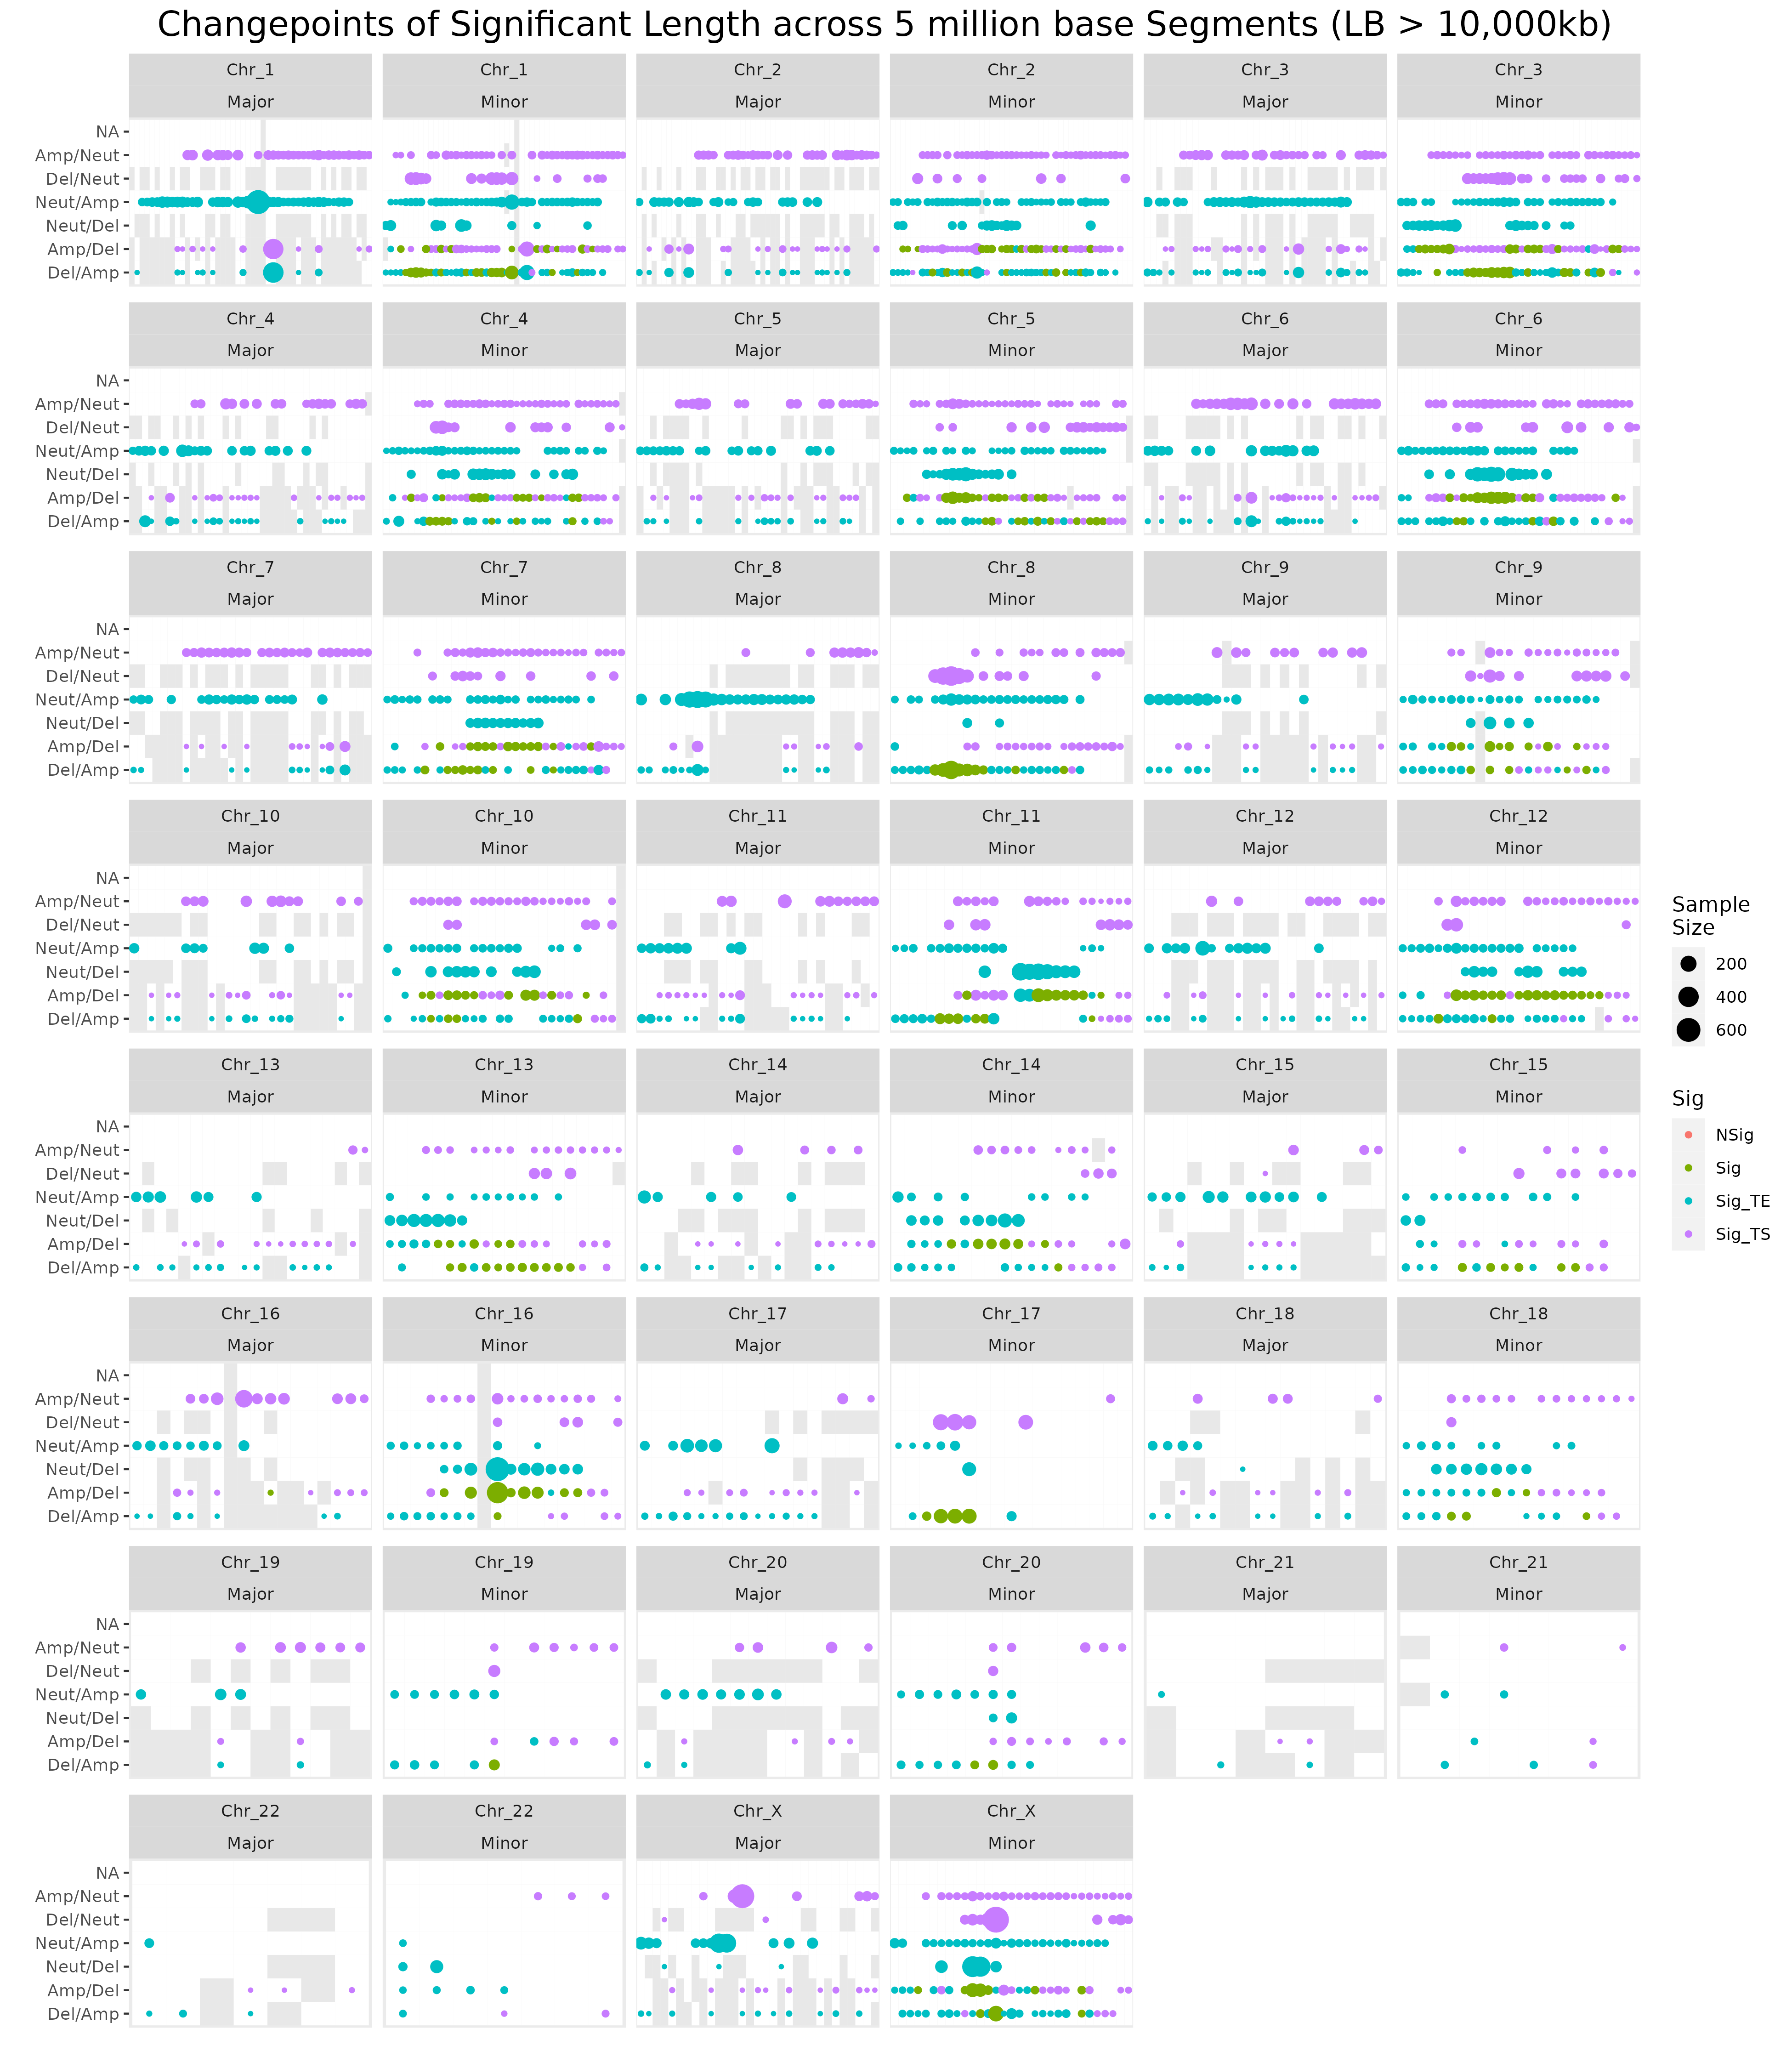
\includegraphics[width = 1\textwidth, height = 22cm]{../figures/Chapter_6/PerSegments_MCMC_10000kb_fivemillion_Thesis.png}
\caption[Application of multivariate Allele Dependent Intercept Model to each segment, providing prediction intervals for each category and allele. Significance determined by $LB > 10,000$kb.]{Application of multivariate Allele Dependent Intercept Model to each segment, providing prediction intervals for each category and allele. Each panel, corresponding to chromosome and allele, displays significance of changepoint, determined by $LB > 10,000$kb. NoCP corresponds to NoChangepoint. Fitted using the \texttt{MCMCglmm()} function.}
\label{fig:PerSegment_MCMC_10000}
\end{figure}

Exploring further the identified points of focus, Neut/Amp changepoint on the Major allele in segment 27 on chromosome 1, Del/Amp changepoint on the Major allele in segment 31 on chromosome 1 and Neut/Del changepoint on the Minor allele in chromosome 16 segment 9, KM survival curves for DSS outcome are produced and compared for patients who exhibit or don't exhibit this particular changepoint profile, Figure \ref{fig:TopLength_Genes_Surv}. Applying the log-rank test for each point of focus, indicates patients with a Neut/Amp changepoint in chromosome 1 segment 27, and patients with a Neut/Del changepoint in chromosome 16 segment 9, have better DSS outcomes than patients that do not exhibit that changepoint ($p < 0.0001$).  This is counter-intuitive as large genomic CNA burden is often associated with worse survival outcome. However, there are a number of explanations for this: the KM curves only consider one type of changepoint at a time, i.e. compares survival of patients who have specific CNA changepoint with patients who do not, even though there could be other changepoints events occurring in a genomic region simultaneously, the KM curves do not consider any other variables such as clinical variables, and whole genome duplication events or changepoints with large lengths occurring in adjacent segments (resulting in CNAs spanning the length of the segment) are not detected.

\vfill
\begin{table}[!htb]
\caption[Genomic segments containing changepoints with $n > 200$ and $LB > 10,000$kb from  models fitted using \texttt{MCMCglmm()} function.]{Genomic segments containing changepoints with $n > 200$ and $LB > 10,000$kb from  models fitted using \texttt{MCMCglmm()} function.}

\centering
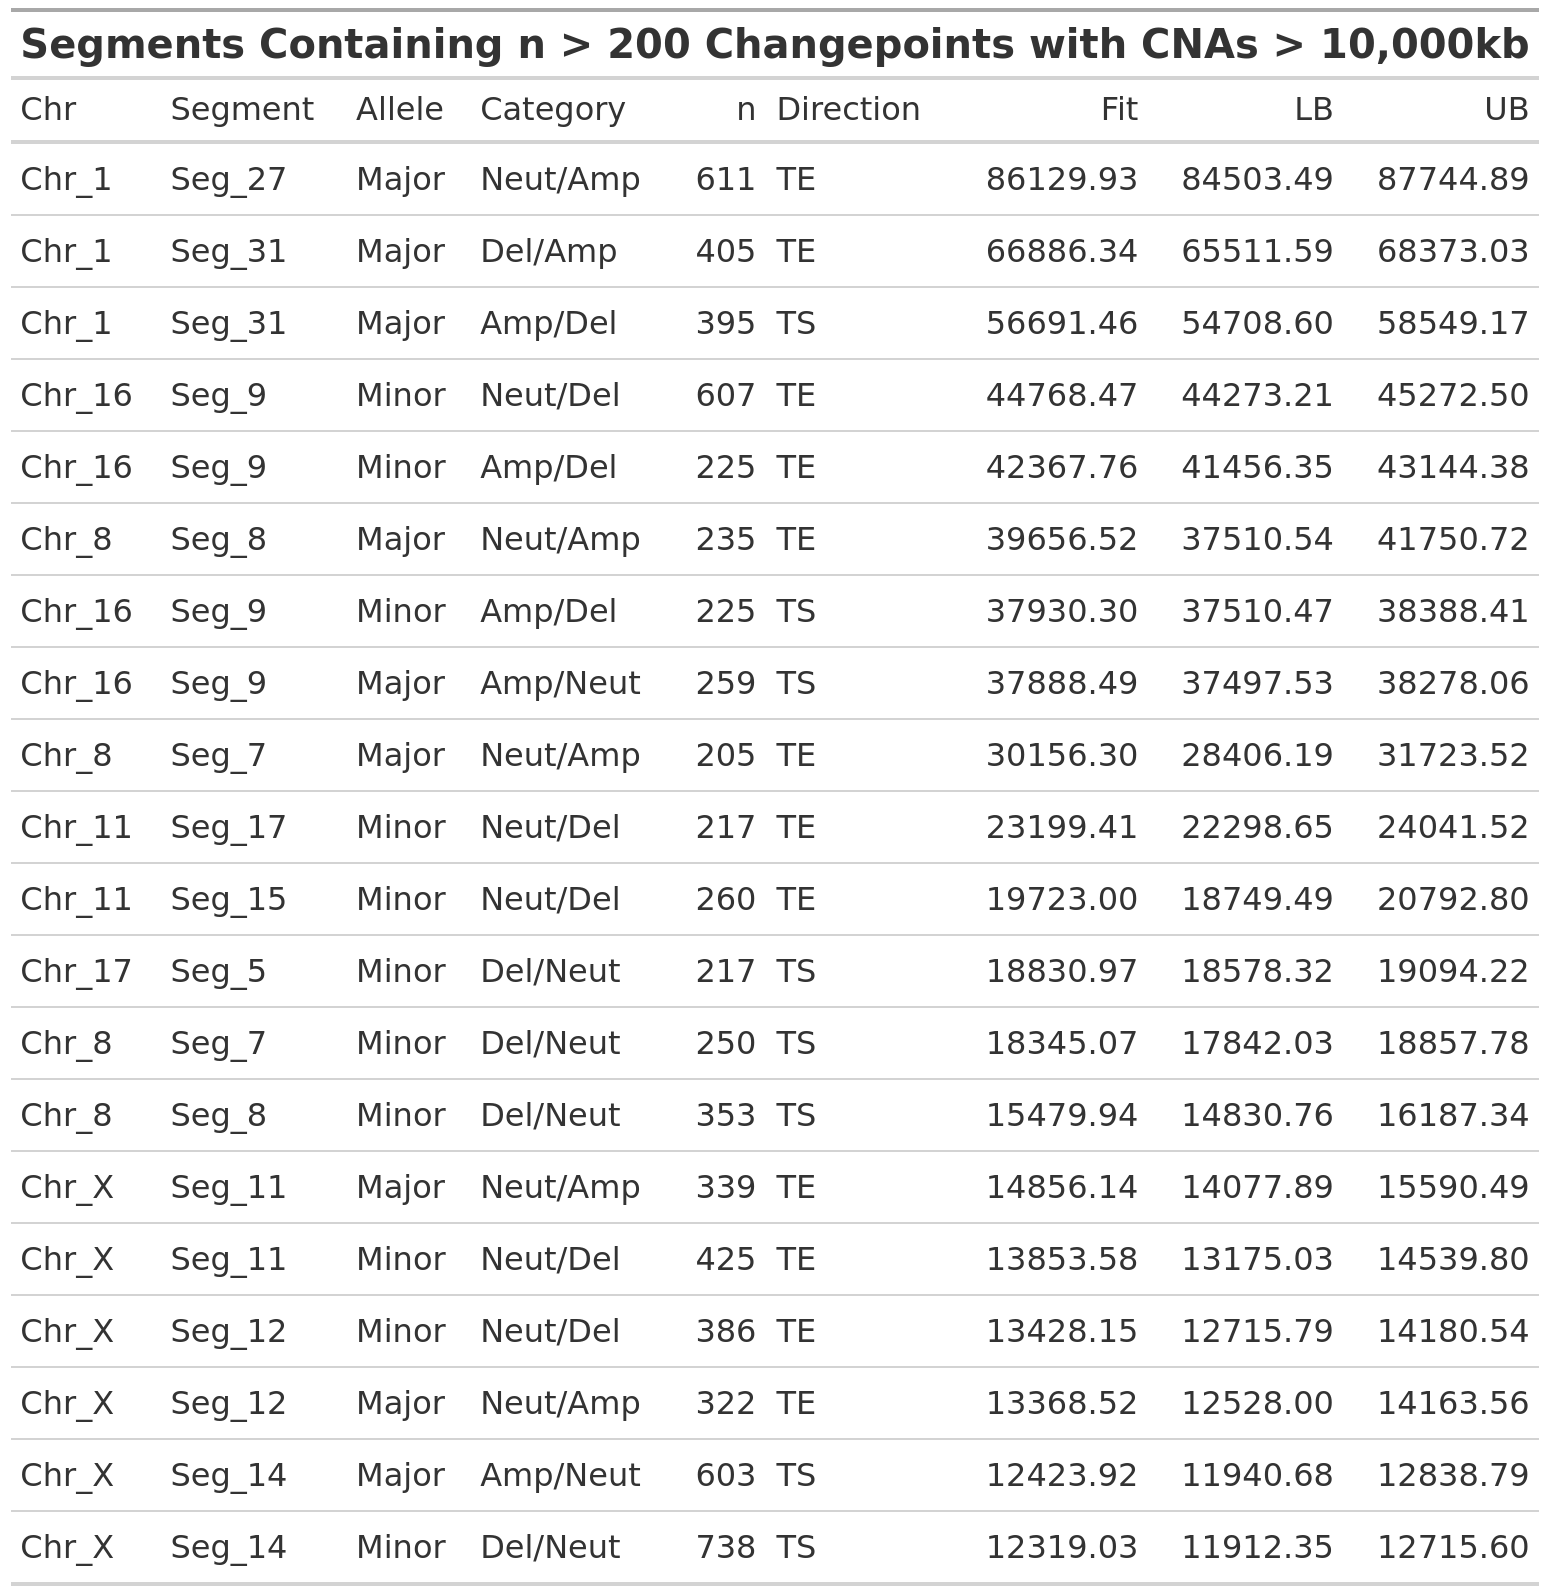
\includegraphics[width = 0.5\textwidth]{../tables/Chapter_6/Segment_MCMC_10000_Five_Thesis.png}
\label{tab:TopLength_Seg_1}
\end{table}
\vfill 

\begin{figure}[!htb]
\centering
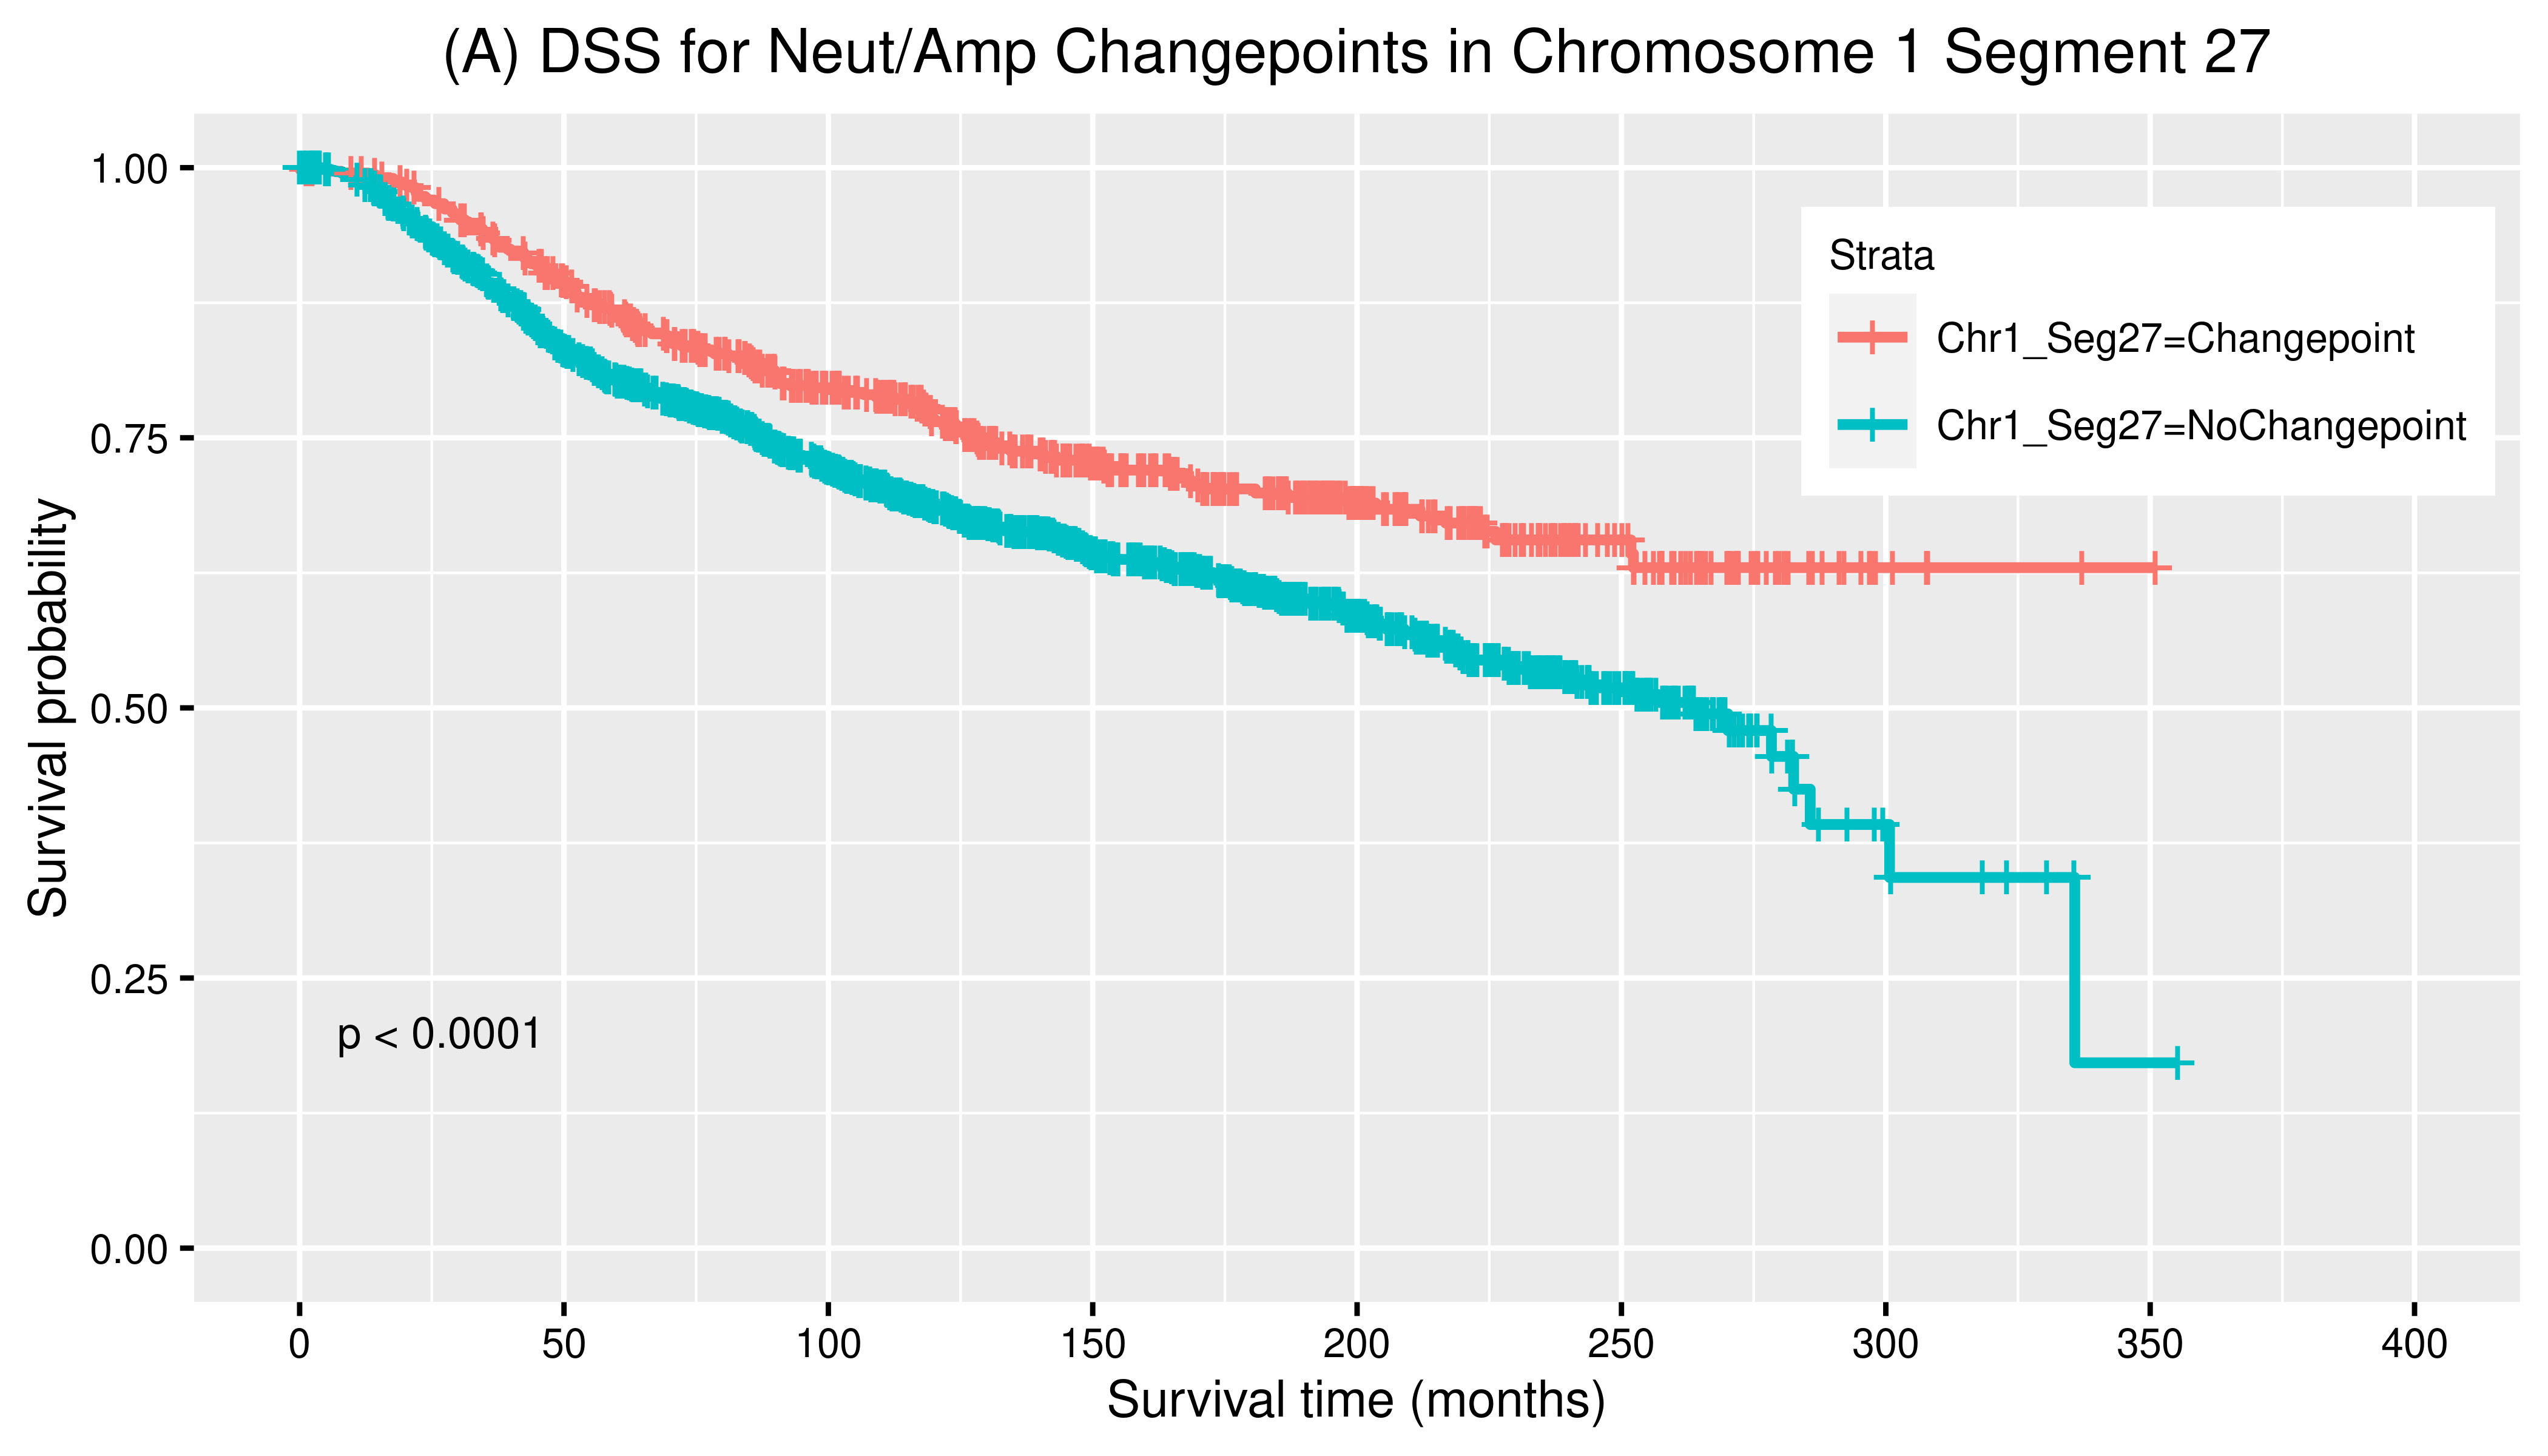
\includegraphics[width = 0.48\textwidth]{../figures/Chapter_6/survplot_Chr1Seg27.png}
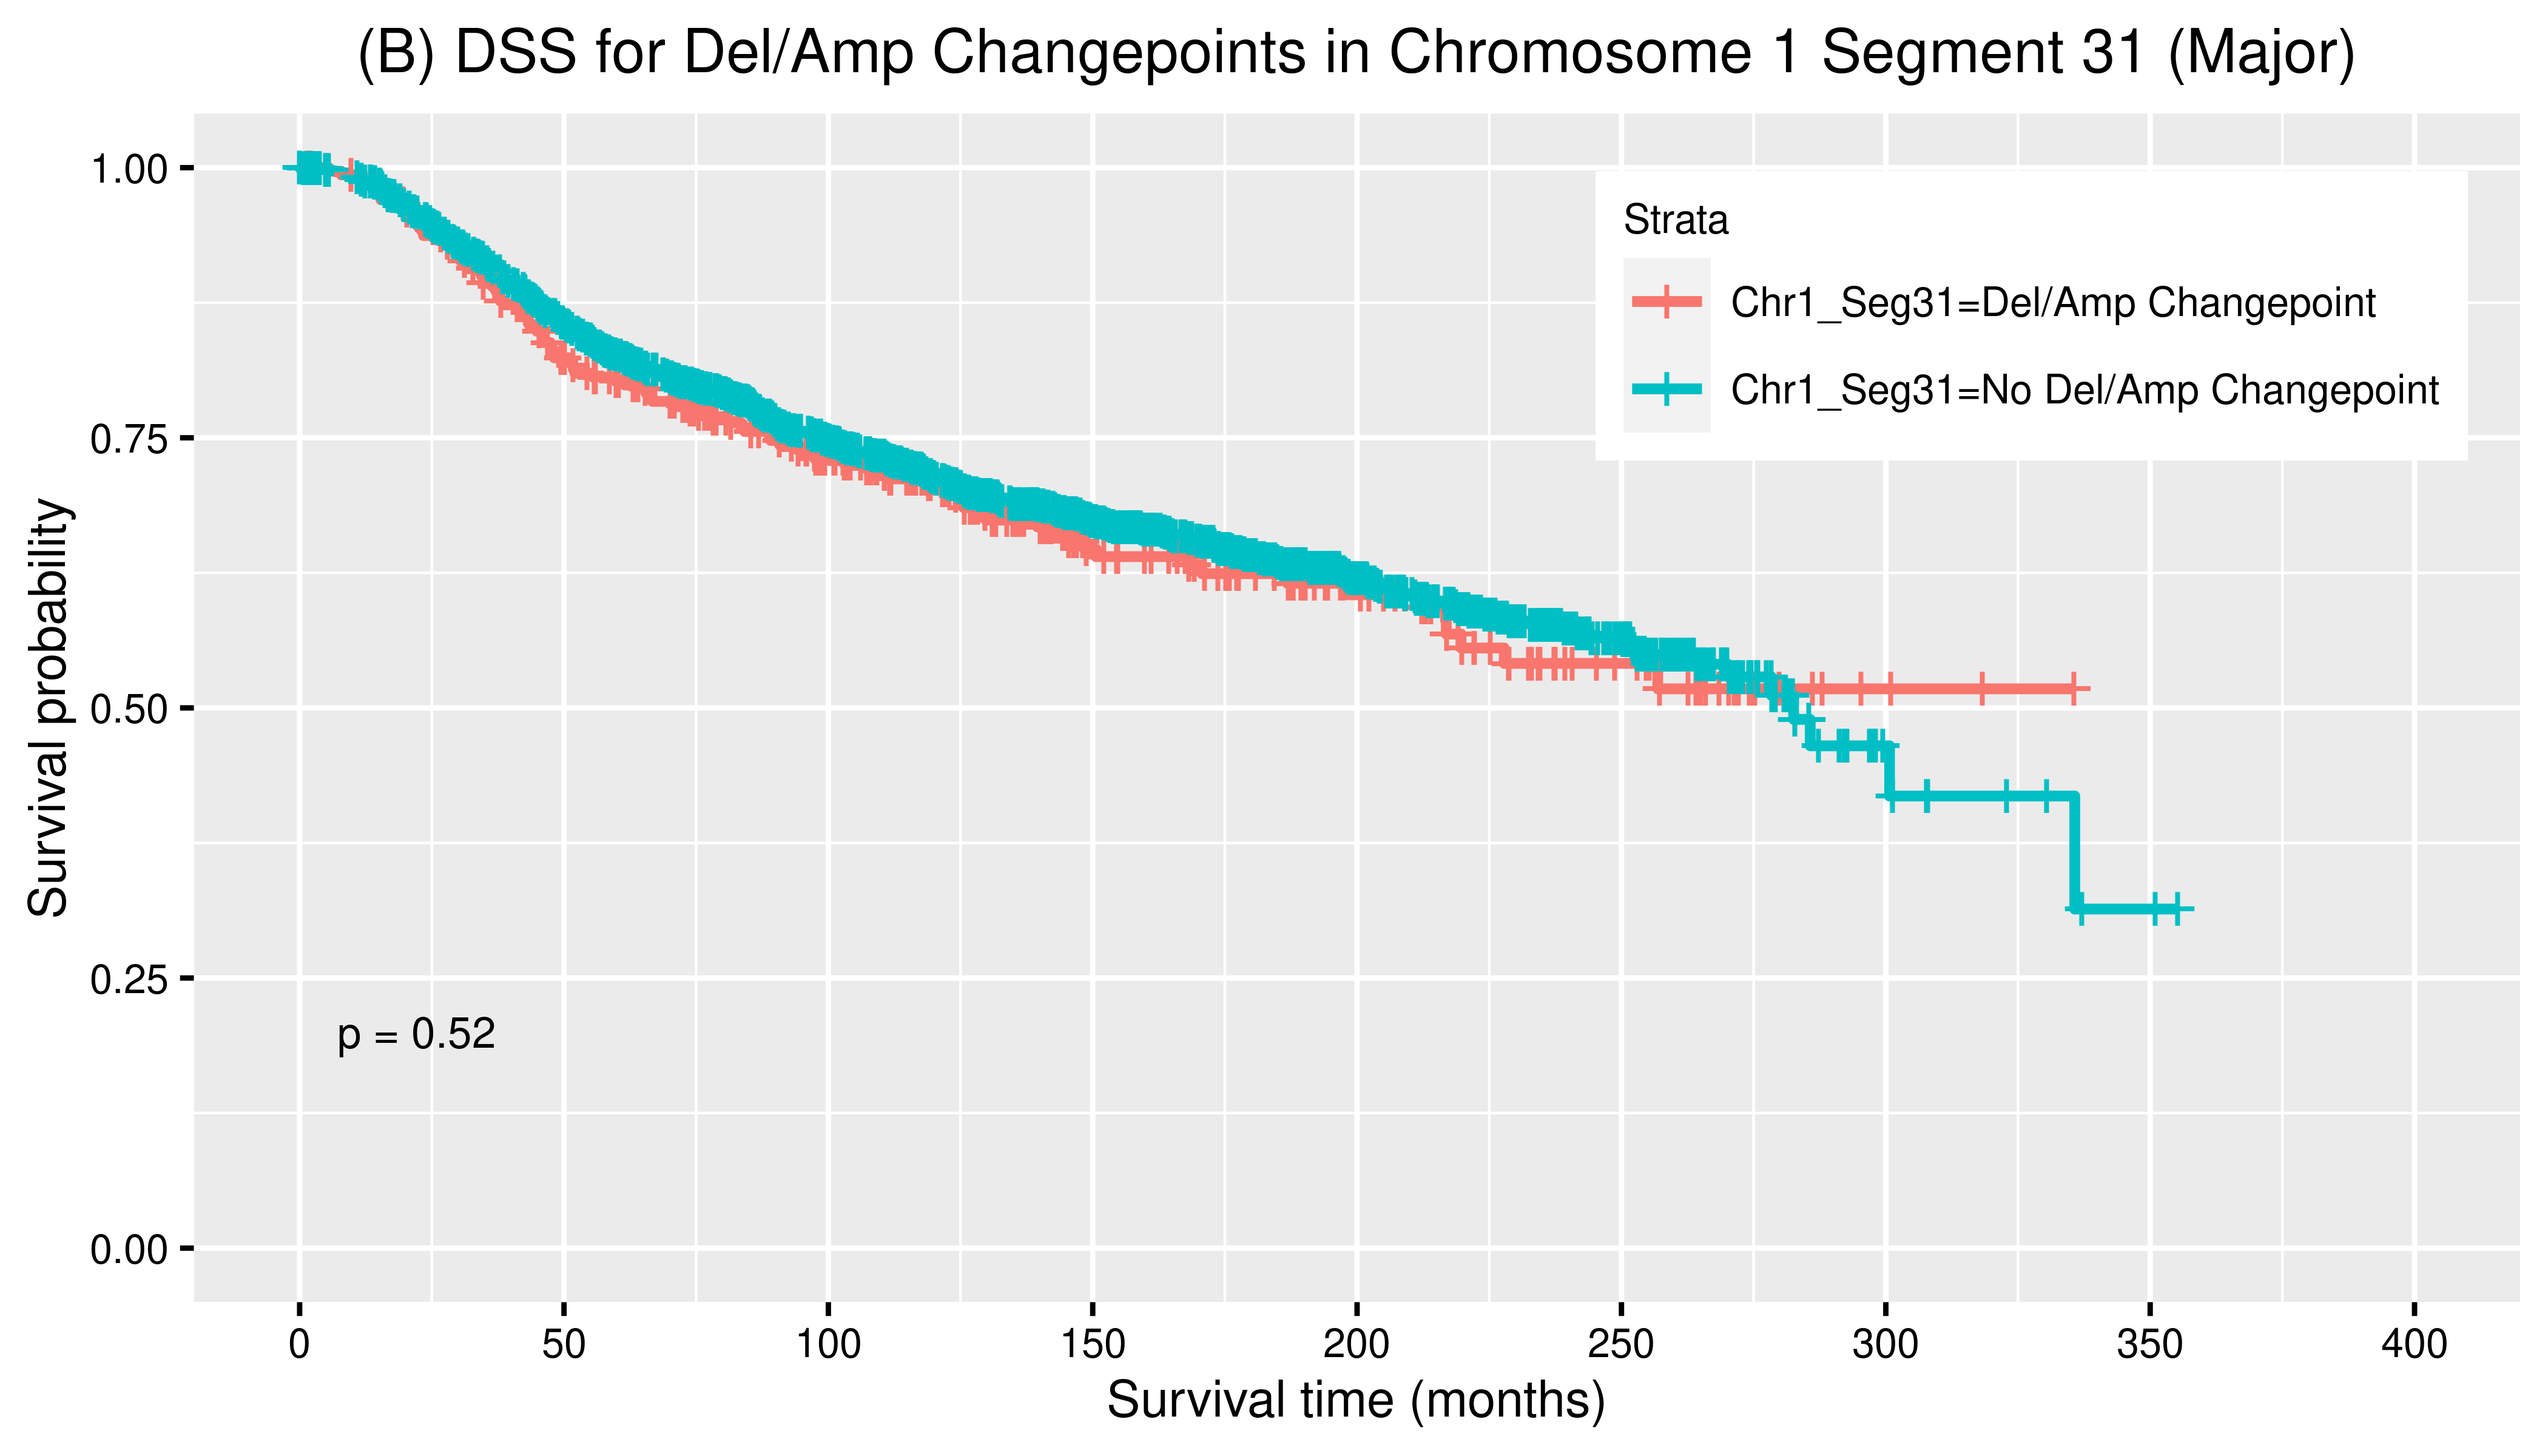
\includegraphics[width = 0.48\textwidth]{../figures/Chapter_6/survplot_Chr1Seg31.png}
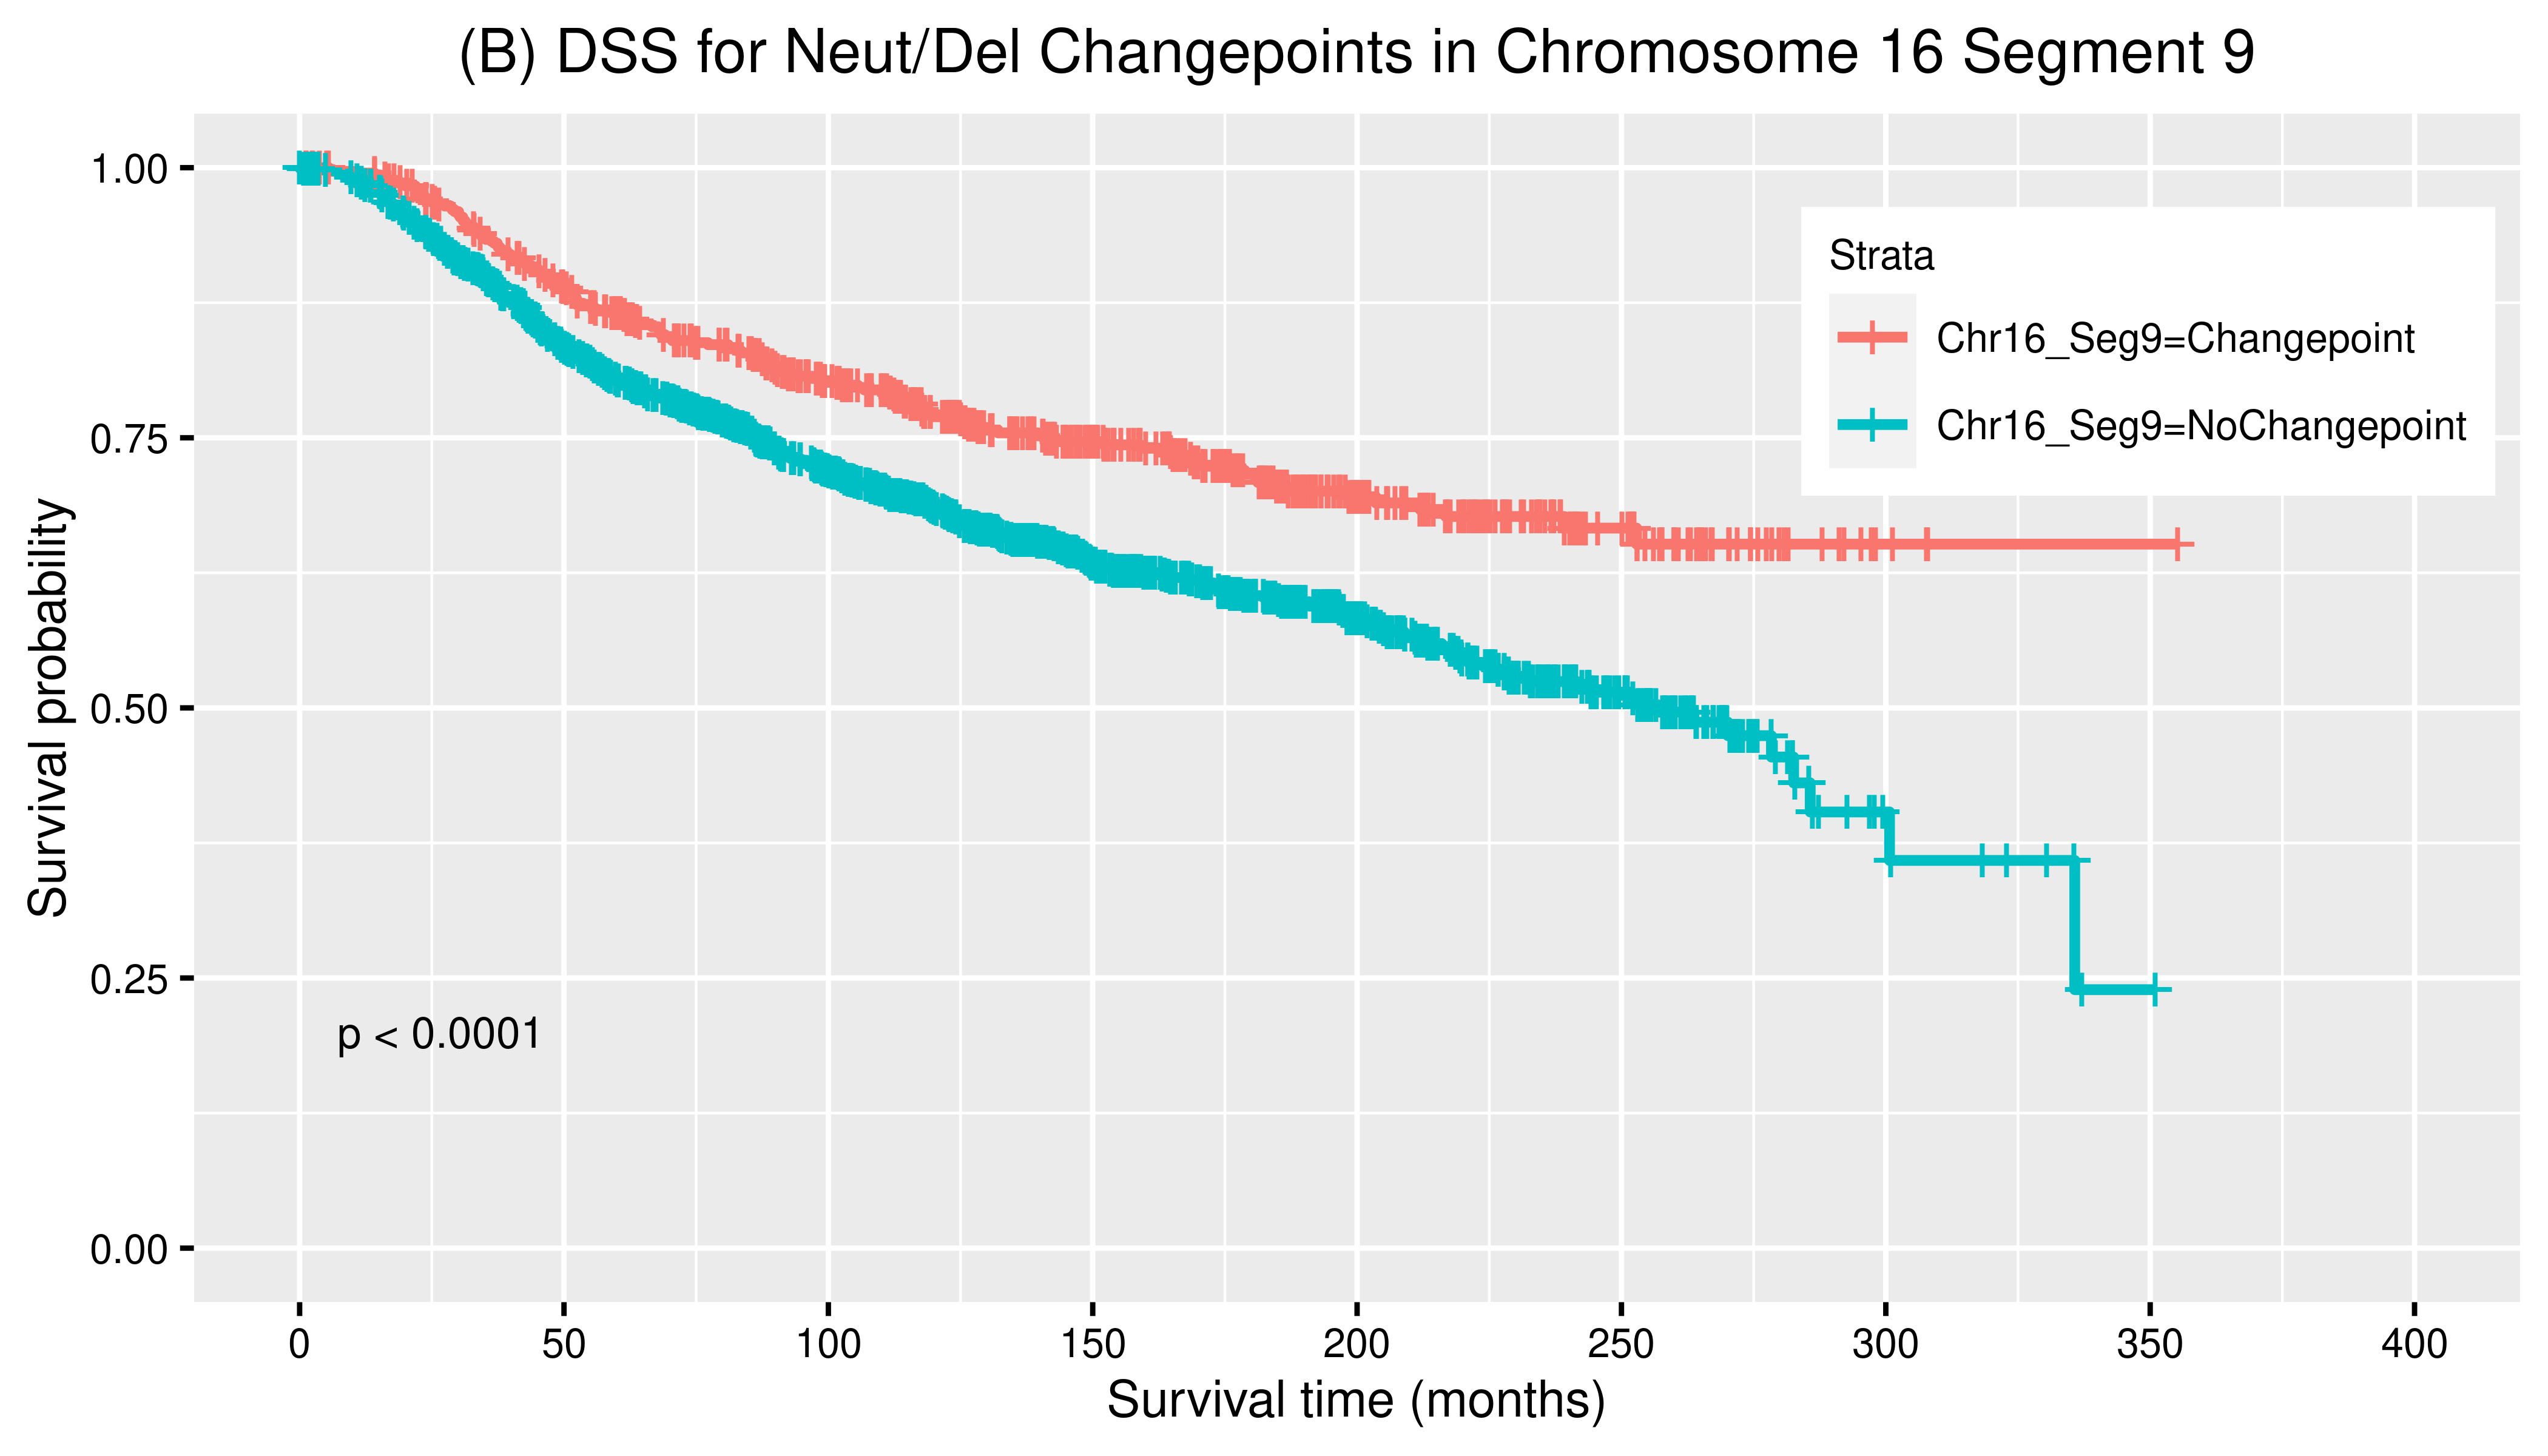
\includegraphics[width = 0.48\textwidth]{../figures/Chapter_6/survplot_Chr16Seg9.png}
\caption[Survival Curves for changepoints in (A) Chromosome 1 Segment 27 (B) Chromosome 1 Segment 31 and (C) Chromosome 16 Segment 9]{Survival Curves for changepoints in (A) Chromosome 1 Segment 27 (B) Chromosome 1 Segment 31 and (C) Chromosome 16 Segment 9.}
\label{fig:TopLength_Segments_Surv}
\end{figure}

\subsection{Conclusion}
Allele-specific copy number profiling provides information on genome wide copy number for each allele and tackles some of the limitations of total copy number profiling, including masking of changepoints and being unable to detect certain types of genomic aberrations, such as LOH and copy number-neutral events.

In this chapter we produced allele-specific copy number profiles, ASCAT profiles, for 1,984 METABRIC patients. Comparing allele-specific copy number profiles to the total copy number profiles, as produced in Chapter 3, using heatmaps of CNA states, similarities were observed, but the allele-specific copy number offered additional insight, by displaying high level of amplifications, possibly indicative of whole genome or chromosome duplication. 

The ADIM was developed in Chapter 5 to identify genomic regions displaying significant changepoints along the allele-specific profile, with significant lengths of state before ($TS$) or after ($TE$) the changepoint. ADIM is applicable within a pre-defined genomic region $d$, and in applying to the METABRIC cohort, we focused on two approaches, a gene-centric application, where $d$ is defined as the region of the gene, and assumed different in size for different genes, and a whole-genome segmentation application, where  $d$ is set to a fixed length and the application searches over consecutive regions of length $d$. These applications ensure whole-genome coverage and identifies specific genes and non-gene regions of interest. KM curves were produced to take an exploratory look at how these changepoints may influence survival outcome. 

Genes including OR52N1, TRIM5, ALG1L2, LCE3B, PRIM2 and EYS were among the genes displaying changepoints, with $>30$ observations, that had an average $TS$ and/or $TE$ length greater than 10,000kb. These genes contain both a changepoint and region(s) of altered copy number, potentially disrupting gene function. Whole genome segments, including chromosome 1 segment 27, chromosome 1 segment 31 and chromosome 6 segment 19, were among the genomic segments displaying changepoints, with $>200$ observations, that had an average $TS$ and/or $TE$ length greater than 10,000kb.

Overall, it is clear that CNAs affect a large proportion of the cancer genome, with these CNAs occurring through whole-region duplication/deletion, or via a copy number change at some point along the genome, resulting in a CNA associated changepoint. 